% !TeX encoding = UTF-8
% Compilare con la ricetta latexmk per aggiornare anche bibliografia e riferimenti.
% !TeX spellcheck = it_IT

% Cerca la classe e il logo direttamente nel pacchetto originale.
% Il percorso va impostato prima che la classe verifichi la presenza del logo.
\makeatletter
\def\input@path{{sapthesis/}}
\makeatother

\documentclass[oneside, noexaminfo]{sapthesis}

\usepackage[italian]{babel}
\usepackage[utf8]{inputenc}
\usepackage{microtype}
\usepackage{listings}
\lstset{
    literate=
        {à}{{\`a}}1 {è}{{\`e}}1 {é}{{\'e}}1 {ì}{{\`i}}1 {ò}{{\`o}}1 {ù}{{\`u}}1
        {À}{{\`A}}1 {È}{{\`E}}1 {É}{{\'E}}1 {Ì}{{\`I}}1 {Ò}{{\`O}}1 {Ù}{{\`U}}1
}
\usepackage{subcaption}
\usepackage{hyperref}
% Numera anche le sottosottosezioni per mantenerne distinti i rimandi.
\setcounter{secnumdepth}{3}
% Mostra anche le sottosottosezioni nell'indice.
\setcounter{tocdepth}{3}
\usepackage{url}
\usepackage{amssymb}
\usepackage{verbatim}
\usepackage{array}
\usepackage{lmodern}
\usepackage[htt]{hyphenat}
\usepackage{booktabs}
\usepackage{graphicx}
\usepackage{tikz}
\usetikzlibrary{positioning, fit, backgrounds, shapes.geometric, shapes.symbols, shapes.arrows, arrows.meta, calc}
\graphicspath{{immagini/}{sapthesis/}}
\hypersetup{
    pdftitle={Titolo della tesi},
    pdfauthor={Lorenzo Mercuri},
    colorlinks=true,
    linkcolor=sapred,
    citecolor=sapred,
    urlcolor=cyan
}


% Frontespizio: sostituire i segnaposto e verificare i dati del corso.
\title{Localizzazione, interpretazione ed analisi computazionale del fotoritocco nella comunicazione politica sui social media}
% \subtitle{Eventuale sottotitolo}
\author{Lorenzo Mercuri}
\IDnumber{2145783}
\course{Laurea Triennale in Informatica}
\courseorganizer{Facoltà di Ingegneria dell'informazione, informatica e statistica}
\AcademicYear{2025/2026}
\advisor{Prof.~Matteo Cinelli}
\customcoadvisorlabel{Relatore esterno}
\coadvisor{Prof.~Mattia Samory}
\authoremail{mercuri.2145783@studenti.uniroma1.it}
\copyyear{2026}
\thesistype{Tesi di laurea}

\begin{document}

\frontmatter
\maketitle


\begin{abstract}
In questa tesi studio l'associazione tra il contenuto delle regioni potenzialmente alterate nelle immagini politiche e l'engagement, cioè le interazioni degli utenti con i post. Realizzo una pipeline che combina il rilevamento e la localizzazione di TruFor, 19 caratteristiche visive dell'immagine, didascalie automatiche e trascrizioni delle scritte nelle regioni selezionate. Rappresento il testo mediante pesi sulle parole e una versione a dimensionalità ridotta. Confronto le informazioni ottenute mediante regressione logistica e modelli lineari generalizzati binomiali.

Analizzo post di Facebook e Instagram del periodo delle elezioni europee del 2024. Il campione finale comprende 1.195 osservazioni, classificate in base a un engagement superiore o inferiore alle aspettative dell'account. La logistica con testo e punteggio TruFor raggiunge il $59{,}4\%$ di accuratezza, contro il $51{,}2\%$ ottenuto assegnando sempre la classe più frequente. Nel confronto fra modelli binomiali, testo e caratteristiche visive aggiunti separatamente migliorano l'indice di validazione rispetto al solo TruFor. La loro combinazione migliora l'adattamento sui dati di stima, ma riduce l'indice in validazione rispetto ai due modelli intermedi.

I risultati indicano una capacità predittiva modesta delle rappresentazioni nel protocollo adottato. La preparazione dei predittori sull'intero campione prima della validazione e l'assenza di suddivisioni per account o periodo limitano le conclusioni sulla generalizzazione. Uso le spiegazioni delle previsioni per ispezionare il modello, mantenendole distinte dagli effetti causali dei contenuti sull'engagement. Il lavoro fornisce uno strumento riutilizzabile e una base per confronti successivi con descrizioni dell'immagine intera e valutazioni su nuovi contesti.
\end{abstract}

\tableofcontents

\mainmatter

% Aggiungere un file per ogni capitolo, nell'ordine definitivo di lettura.
% La numerazione dei capitoli viene assegnata automaticamente.
% !TeX root = ../tesi.tex
% !TeX encoding = UTF-8
% !TeX spellcheck = it_IT

\chapter{Introduzione}
\label{chap:introduzione}

I social network costituiscono uno spazio rilevante della comunicazione politica. Le immagini contribuiscono alla presentazione dei candidati e dei loro messaggi: il ritocco e l'aggiunta di elementi grafici o testuali fanno parte di questa costruzione. Tali modifiche possono avere una funzione comunicativa anche senza un intento ingannevole. Studio il loro rapporto con l'\emph{engagement}, cioè le interazioni degli utenti con i post, per comprendere come il pubblico partecipa alla comunicazione politica online.

Gli strumenti forensi come TruFor permettono di rilevare e localizzare possibili manipolazioni~\cite{Guillaro_2023_CVPR}. Il punteggio e le mappe segnalano indizi forensi, ma non descrivono il messaggio contenuto nelle regioni individuate. Resta quindi da verificare quale relazione intercorra tra questo contenuto e l'engagement. Per esaminarla occorre descrivere le regioni segnalate e collegare le informazioni ottenute ai dati sulle interazioni.

Affronto questa domanda: \emph{quanto contribuiscono il contenuto delle regioni potenzialmente alterate e le caratteristiche visive alla classificazione dell'engagement, rispetto al solo punteggio TruFor?} Considero post politici pubblicati su Facebook e Instagram nel periodo delle elezioni europee del 2024. Uso l'indicatore di CrowdTangle per distinguere i post con engagement superiore o inferiore alle aspettative dell'account~\cite{DVN/SCCQYD_2019}, secondo la definizione del Capitolo~\ref{chap:dataset}.

Presento l'approccio e il contributo nella Sezione~\ref{sec:introduzione-approccio}; nella Sezione~\ref{sec:introduzione-organizzazione} sintetizzo i risultati, le implicazioni e la struttura della tesi.

\section{Approccio e contributo}
\label{sec:introduzione-approccio}

L'elemento distintivo del progetto consiste nel descrivere le regioni potenzialmente modificate, anziché l'immagine nel suo insieme. Questa scelta offre una base per formulare ipotesi sul ruolo comunicativo delle modifiche a partire dai contenuti segnalati dal rilevatore.

Realizzo una pipeline che applica alle immagini una maschera ricavata dalle mappe di TruFor~\cite{Guillaro_2023_CVPR}. Descrivo il contenuto conservato con BLIP (Bootstrapping Language-Image Pre-training)~\cite{pmlr-v162-li22n} e aggiungo le scritte lette mediante OCR (Optical Character Recognition)~\cite{easyocr_software}. Trasformo il testo in vettori numerici e in una versione a dimensionalità ridotta. Affianco a queste rappresentazioni il punteggio globale di TruFor e 19 caratteristiche visive estratte dall'immagine intera.

Confronto le combinazioni dei tre blocchi informativi mediante modelli lineari generalizzati, GLM (Generalized Linear Models), della famiglia binomiale~\cite{68aee965-a8a0-3e72-9f89-8d89ae91a62b}. Affianco una regressione logistica regolarizzata per la classificazione e strumenti che rendono leggibile il contributo delle parole alle previsioni.

Il contributo comprende lo strumento di analisi automatizzata, il codice riutilizzabile e lo studio esplorativo sul campione politico. Integro modelli forensi e linguistici già addestrati nel procedimento riassunto nella Figura~\ref{fig:pipeline-generale}.

\begin{figure}[htbp]
    \centering
    \begin{tikzpicture}[
        blocco/.style={draw=black!65, rounded corners=2pt, align=center,
            font=\small, text width=2.5cm, minimum height=0.85cm, inner sep=5pt},
        dato/.style={blocco, fill=black!4},
        modulo/.style={blocco, fill=sapred!20},
        flusso/.style={-{Stealth[length=2mm]}, semithick, draw=black!70}
    ]
        \node[dato, text width=4.4cm] (post) at (0,0)
            {Post e immagini\\Facebook e Instagram};
        \node[modulo, text width=4.4cm] (filtro) at (0,-1.3)
            {Filtraggio\\del campione};
        \node[dato] (immagini) at (0,-2.6) {Immagini};
        \node[dato, text width=3cm] (engagement) at (4,-2.6)
            {Engagement\\CrowdTangle};
        \node[modulo] (trufor) at (-2,-4) {TruFor};
        \node[modulo] (visive) at (2,-4) {Analisi visiva};
        \node[dato] (punteggio) at (-4,-5.5) {Punteggio globale};
        \node[dato] (mappe) at (-0.7,-5.5)
            {Mappe TruFor};
        \node[dato, text width=3cm] (caratteristiche) at (3.1,-5.5)
            {Caratteristiche\\visive (19)};
        \node[modulo, text width=3.2cm] (descrizione) at (-0.7,-7)
            {Maschera,\\BLIP e OCR};
        \node[dato, text width=3.2cm] (testo) at (-0.7,-8.5)
            {Rappresentazioni\\numeriche del testo};
        \node[modulo, text width=7cm, minimum height=1.2cm] (modelli) at (0,-10.1)
            {Classificazione dell'engagement\\Confronto dei blocchi informativi,\\validazione e interpretazione};

        \draw[flusso] (post) -- (filtro);
        \draw[flusso] (filtro) -- (immagini);
        \draw[flusso] (filtro.east) -| (engagement.north);
        \draw[flusso] (immagini.south) -- ++(0,-0.2) -| (trufor.north);
        \draw[flusso] (immagini.south) -- ++(0,-0.2) -| (visive.north);
        \draw[flusso] (trufor.south) -- ++(0,-0.2) -| (punteggio.north);
        \draw[flusso] (trufor.south) -- ++(0,-0.2) -| (mappe.north);
        \draw[flusso] (visive.south) -- ++(0,-0.2) -| (caratteristiche.north);
        \draw[flusso] (mappe) -- (descrizione);
        \draw[flusso] (descrizione) -- (testo);
        \draw[flusso] (testo.south) -- (testo.south |- modelli.north);
        \draw[flusso] (punteggio.south) -- (-4,-9.25) -| ([xshift=-2.7cm]modelli.north);
        \draw[flusso] (caratteristiche.south) -- (caratteristiche.south |- modelli.north);
        \draw[flusso] (engagement.east) -- ++(0.4,0) |- (modelli.east);
    \end{tikzpicture}
    \caption{Schema della pipeline. I riquadri colorati indicano le elaborazioni; quelli grigi i dati. Le mappe TruFor guidano la selezione delle regioni da descrivere; estraggo le caratteristiche visive dall'immagine intera. Confronto i tre blocchi informativi usando l'engagement di CrowdTangle per definire le classi di riferimento.}
    \label{fig:pipeline-generale}
\end{figure}

\section{Risultati, implicazioni e struttura della tesi}
\label{sec:introduzione-organizzazione}

Nelle analisi del solo punteggio di manipolazione osservo un'associazione debole con l'engagement, non statisticamente significativa alla soglia del $5\%$. Sul campione finale di 1.195 osservazioni la logistica con testo e punteggio TruFor raggiunge il $59{,}4\%$ di accuratezza, contro il $51{,}2\%$ ottenuto assegnando sempre la classe più frequente. Nel confronto fra GLM, l'aggiunta del testo o delle caratteristiche visive migliora l'indice di validazione rispetto al solo TruFor. La combinazione di entrambi i blocchi migliora l'adattamento ai dati di addestramento, ma ottiene risultati inferiori in validazione rispetto alle due aggiunte separate.

Il confronto sostiene una capacità predittiva modesta e indica che il contenuto descritto e l'aspetto generale dell'immagine aggiungono informazioni utili al punteggio di manipolazione. La preparazione dei dati usa però l'intero campione prima della validazione e le suddivisioni non separano account o periodi. Interpreto quindi gli esiti come esplorativi. Spiego questi risultati come associazioni tra le informazioni ricavate dalle immagini e l’engagement osservato.

Il lavoro può aiutare chi analizza le campagne sui social network a valutare le scelte visive sulla base di riscontri empirici. Applicare lo strumento ad altre raccolte di immagini associate a dati di engagement permette di confrontare campagne, periodi e contesti diversi. Questo riutilizzo consente di verificare quali relazioni si ripresentino e quali siano specifiche del caso esaminato.

Nel Capitolo~\ref{chap:background} presento gli strumenti e i riferimenti teorici. Nel Capitolo~\ref{chap:dataset} descrivo dati, rappresentazioni e misure. Nel Capitolo~\ref{chap:metodi} illustro la pipeline e il protocollo di valutazione; nel Capitolo~\ref{chap:risultati} riporto gli esiti. Concludo con la discussione nel Capitolo~\ref{chap:discussione}, i limiti e gli sviluppi futuri nel Capitolo~\ref{chap:limiti}, e la sintesi dei contributi nel Capitolo~\ref{chap:conclusioni}.

% !TeX root = ../tesi.tex
% !TeX encoding = UTF-8
% !TeX spellcheck = it_IT

\chapter{Background e lavori correlati}
\label{chap:background}

In questo capitolo presento TruFor, il sistema che utilizzo per studiare le manipolazioni. TruFor è un framework per l'analisi \emph{forense} delle immagini, cioè l'esame delle tracce lasciate dall'acquisizione e dalle elaborazioni successive, per individuare possibili manipolazioni. Introduco i compiti dell'analisi forense e descrivo il funzionamento di TruFor. Esamino poi i risultati e i limiti che gli autori riportano nel loro lavoro. Uso questi elementi per motivare la scelta del sistema nello studio della comunicazione politica sui social media.

Presento poi gli strumenti statistici per l'analisi delle associazioni e i descrittori visivi che adopero per rappresentare le caratteristiche dell'immagine. Infine introduco gli strumenti per il riconoscimento ottico dei caratteri, e per descrivere il contenuto delle regioni sospette.

\section{TruFor}
\label{sec:background-trufor}

\subsection{Rilevamento e localizzazione delle manipolazioni}
\label{sec:background-rilevamento-localizzazione}

Isolo due compiti dell'analisi. Il \emph{rilevamento} classifica un'immagine come autentica o manipolata. La \emph{localizzazione} indica le regioni che il sistema segnala come manipolate. Descrivo questo compito con una \emph{segmentazione binaria}: il sistema assegna ciascun pixel alla classe ``autentico'' o ``manipolato''~\cite{Guillaro_2023_CVPR}.

Osservo manipolazioni come il copia-incolla e l'inserimento di contenuti sintetici.

Valuto positiva la classe ``manipolato'' e negativa la classe ``autentico''. Questa convenzione vale sia per le immagini nel rilevamento sia per i pixel nella localizzazione. TruFor può segnalare come manipolate anche regioni autentiche, producendo falsi positivi a livello di pixel. Nel rilevamento, i falsi positivi possono costituire una parte consistente delle segnalazioni quando le manipolazioni sono poco frequenti. Quando interpreto i risultati, distinguo quindi gli errori di localizzazione dagli errori di rilevamento.

\subsection{Indizi visivi e impronta Noiseprint++}
\label{sec:background-noiseprint}

L'immagine RGB descrive il contenuto visibile; l'\emph{estrattore Noiseprint++} genera un'impronta, \emph{Noiseprint++}, che evidenzia le incoerenze tra le tracce presenti nelle diverse regioni. Trufor combina la fotografia con la sua impronta.

Noiseprint++ estende \emph{Noiseprint}, un'impronta che rappresenta le tracce dei processi interni alla fotocamera. Noiseprint++ include anche le tracce delle elaborazioni successive all'acquisizione. L'addestramento dell'estrattore di impronta avviene con immagini autentiche. L'addestramento è auto-supervisionato: gli autori ricavano il segnale di apprendimento dalle relazioni tra gli esempi.

Gli autori utilizzano 24.700 immagini acquisite con 1.475 modelli di fotocamera. Ne estraggono porzioni di $64 \times 64$ pixel. L'addestramento segue un criterio \emph{contrastivo}: produce impronte simili nelle aree che condividono le stesse proprietà e diverse nelle aree che differiscono. Le proprietà richieste sono il modello di fotocamera, la posizione nello spazio e la storia delle elaborazioni. Gli sviluppatori simulano quest'ultima con 512 combinazioni di ridimensionamento, compressione e variazioni di illuminazione.

\subsection{Architettura e apprendimento}
\label{sec:background-trufor-architettura}

Il sistema elabora l'RGB e Noiseprint++ attraverso due rami. Ogni ramo estrae delle \emph{caratteristiche}, rappresentazioni numeriche delle informazioni della figura. La fusione delle caratteristiche usa una rete di tipo \emph{Transformer}, che apprende relazioni tra gli elementi delle rappresentazioni.

L'\emph{encoder} estrae le caratteristiche che alimentano due \emph{decoder}. Ciascun decoder produce una mappa con la stessa risoluzione della fotografia.

Il decoder delle anomalie produce la \emph{mappa delle anomalie}, che assegna a ciascun pixel un valore che esprime quanto il sistema lo considera sospetto. I valori alti indicano le regioni segnalate come manipolate. Pixel autentici possono ricevere valori alti e generare falsi positivi.

Il decoder della confidenza produce la \emph{mappa di confidenza}, che stima l'affidabilità della previsione della mappa delle anomalie per ciascun pixel. Una confidenza alta indica che il sistema considera affidabile la previsione. La confidenza riguarda entrambe le classi: ``autentico'' e ``manipolato''.

Riassumo nella Figura~\ref{fig:trufor-mappe} il percorso dall'immagine alle due mappe.

\begin{figure}[htbp]
    \centering
    \begin{tikzpicture}[
        blocco/.style={draw=black!65, rounded corners=2pt, align=center,
            font=\small, text width=2.5cm, minimum height=0.85cm, inner sep=5pt},
        dato/.style={blocco, fill=black!4},
        modulo/.style={blocco, fill=sapred!20},
        flusso/.style={-{Stealth[length=2mm]}, semithick, draw=black!70}
    ]
        \node[dato] (rgb) at (-3.5,0) {Immagine RGB};
        \node[modulo] (estrattore) at (0,0) {Estrattore\\Noiseprint++};
        \node[dato] (impronta) at (3.5,0) {Impronta\\Noiseprint++};
        \node[modulo, text width=4.4cm] (encoder) at (0,-1.6)
            {Encoder a due rami\\e fusione delle caratteristiche};
        \node[modulo] (anomalie) at (-2,-3.1) {Decoder\\delle anomalie};
        \node[modulo] (confidenza) at (2,-3.1) {Decoder\\della confidenza};
        \node[dato] (mappaa) at (-2,-4.4) {Mappa\\delle anomalie};
        \node[dato] (mappac) at (2,-4.4) {Mappa\\di confidenza};
        \draw[flusso] (rgb) -- (estrattore);
        \draw[flusso] (estrattore) -- (impronta);
        \draw[flusso] (rgb.south) |- (encoder.west);
        \draw[flusso] (impronta.south) |- (encoder.east);
        \draw[flusso] (encoder.south) -- ++(0,-0.15) -| (anomalie.north);
        \draw[flusso] (encoder.south) -- ++(0,-0.15) -| (confidenza.north);
        \draw[flusso] (anomalie) -- (mappaa);
        \draw[flusso] (confidenza) -- (mappac);
    \end{tikzpicture}
    \caption{Dall'immagine alle mappe di TruFor. I riquadri colorati rappresentano i componenti appresi; quelli grigi rappresentano i dati. Schema semplificato dalla Figura~2~\cite{Guillaro_2023_CVPR}.}
    \label{fig:trufor-mappe}
\end{figure}

\newpage
Gli autori addestrano TruFor in tre fasi, che riassumo nella Tabella~\ref{tab:trufor-addestramento}. La prima usa il criterio contrastivo descritto nella Sezione~\ref{sec:background-noiseprint}. Nella seconda usano un apprendimento \emph{supervisionato}: gli autori accompagnano gli esempi con le risposte di riferimento. Per ogni istantanea una \emph{maschera di riferimento}, o \emph{ground truth}, indica la classe ``autentico'' o ``manipolato'' di ciascun pixel.

Nella terza fase il decoder della confidenza apprende come stimare la \emph{True Class Probability}, la probabilità che il modello assegna alla classe corretta di ciascun pixel. Questa quantità assume valori alti quando la previsione favorisce la classe corretta. Il decoder della confidenza apprende così come stimare l'affidabilità della mappa delle anomalie.

\begin{table}[htbp]
    \centering
    \small
    \caption{Le tre fasi di addestramento di TruFor~\cite{Guillaro_2023_CVPR}.}
    \label{tab:trufor-addestramento}
    \begin{tabular}{@{}p{0.07\linewidth}p{0.35\linewidth}p{0.49\linewidth}@{}}
        \toprule
        Fase & Componenti addestrati & Obiettivo \\
        \midrule
        1 & Estrattore Noiseprint++ & Produrre impronte simili per porzioni con lo stesso modello di fotocamera, posizione e storia delle elaborazioni. \\
        \addlinespace
        2 & Encoder e decoder delle anomalie & Assegnare a ciascun pixel la classe indicata dalla maschera di riferimento. \\
        \addlinespace
        3 & Decoder della confidenza e classificatore & Stimare l'affidabilità delle previsioni per pixel e riconoscere le immagini manipolate. \\
        \bottomrule
    \end{tabular}
\end{table}

\subsection{Output e loro interpretazione}
\label{sec:background-trufor-output}

TruFor restituisce la mappa delle anomalie e la mappa di confidenza, definite nella Sezione~\ref{sec:background-trufor-architettura}, insieme a un punteggio globale.

La visualizzazione della mappa delle anomalie come mappa di calore evidenzia le regioni da esaminare. Interpreto queste regioni insieme alla mappa di confidenza, per distinguere le segnalazioni che il sistema considera affidabili da quelle che richiedono cautela.

Nel confronto con la letteratura, gli scienziati osservano che numerosi metodi ricavano la valutazione dell'intera fotografia dalle previsioni sui singoli pixel. Gli errori nelle previsioni locali possono così portare a segnalare come manipolata un'immagine autentica. TruFor usa la mappa di confidenza per ridurre il peso delle previsioni meno affidabili.

Il \emph{punteggio globale}, o \emph{integrity score}, esprime la valutazione sul media nel suo complesso. TruFor calcola le statistiche, come media e massimo, delle mappe attraverso il \emph{pooling}, un'operazione di aggregazione. Il classificatore usa queste informazioni per calcolare il punteggio globale.

Nell'interpretazione seguo la priorità proposta dagli autori: considero prima il punteggio globale e poi esamino le mappe dei casi segnalati.

\subsection{Risultati riportati e confronto con la letteratura}
\label{sec:background-trufor-risultati}

Esamino i risultati per valutare due proprietà: la \emph{generalizzazione}, la capacità di riconoscere manipolazioni diverse da quelle di addestramento, e la \emph{robustezza}, la capacità di mantenere le prestazioni dopo trasformazioni dell'immagine. Gli esperimenti comprendono fotoritocchi e manipolazioni locali prodotte con modelli generativi.

Confronto TruFor con \emph{CAT-Net v2}, una rete neurale che combina il contenuto RGB e le tracce della compressione JPEG per localizzare le manipolazioni. Negli esperimenti CAT-Net v2 occupa il secondo posto per F1-score medio a livello di pixel. Riporto il confronto nella Tabella~\ref{tab:trufor-medie}~\cite{Guillaro_2023_CVPR}.

Per la localizzazione, l'F1-score combina precisione e richiamo a livello di pixel. Per il rilevamento, l'AUC (Area Under the Curve) misura l'area sotto la curva ROC (Receiver Operating Characteristic), che mette in relazione i tassi di veri e falsi positivi al variare della soglia. L'accuratezza bilanciata misura invece la media delle percentuali di riconoscimento delle due classi. Valori maggiori indicano prestazioni migliori per tutte e tre le metriche.

\begin{table}[htbp]
    \centering
    \small
    \caption{Prestazioni medie riportate: localizzazione su otto dataset e rilevamento su sette. Fonte: Tabelle~1 e~2~\cite{Guillaro_2023_CVPR}.}
    \label{tab:trufor-medie}
    \begin{tabular}{@{}llrr@{}}
        \toprule
        Compito e metrica & Soglia & TruFor & CAT-Net v2 \\
        \midrule
        Localizzazione: F1-score & Ottimale per immagine & $0{,}785$ & $0{,}709$ \\
        Localizzazione: F1-score & Fissa a $0{,}5$ & $0{,}696$ & $0{,}601$ \\
        Rilevamento: AUC & Variabile & $0{,}857$ & $0{,}797$ \\
        Rilevamento: acc. bilanciata & Fissa a $0{,}5$ & $0{,}781$ & $0{,}649$ \\
        \bottomrule
    \end{tabular}
\end{table}

TruFor supera CAT-Net v2 nelle quattro medie. Separo i risultati con soglia fissa da quelli con soglia ottimale: gli autori scelgono quest'ultima massimizzando l'F1-score per ogni figura, usando la maschera di riferimento. La soglia fissa permette invece di valutare le previsioni puntuali senza questa scelta specifica.

Distinguo due dataset: \emph{OpenForensics} contiene manipolazioni locali di volti basate su reti generative avversarie GAN (Generative Adversarial Networks); \emph{CocoGlide} include manipolazioni locali prodotte con \emph{GLIDE}, un modello a diffusione. La Tabella~\ref{tab:trufor-generative} mostra i risultati per questi dataset.

\begin{table}[htbp]
    \centering
    \small
    \caption{F1-score di localizzazione per dataset e metodo. Il grassetto indica il valore maggiore fra i due metodi per ciascun dataset e soglia. Fonte: Tabella~1~\cite{Guillaro_2023_CVPR}.}
    \label{tab:trufor-generative}
    \begin{tabular}{@{}llrr@{}}
        \toprule
        Dataset e generazione & Metodo & \shortstack{Soglia ottimale\\per immagine} & \shortstack{Soglia fissa\\a $0{,}5$} \\
        \midrule
        OpenForensics (GAN) & TruFor & $0{,}901$ & $0{,}827$ \\
                            & CAT-Net v2 & $\mathbf{0{,}947}$ & $\mathbf{0{,}899}$ \\
        \addlinespace
        CocoGlide (diffusione) & TruFor & $\mathbf{0{,}720}$ & $\mathbf{0{,}523}$ \\
                              & CAT-Net v2 & $0{,}603$ & $0{,}434$ \\
        \bottomrule
    \end{tabular}
\end{table}

CAT-Net v2 supera TruFor su OpenForensics; TruFor supera CAT-Net v2 su CocoGlide. Il vantaggio medio di TruFor comprende quindi risultati diversi sui singoli dataset. Questi esperimenti valutano l'individuazione delle regioni manipolate su due raccolte diverse: il confronto diretto tra GAN e diffusione richiede di controllare anche i contenuti di partenza e le manipolazioni.

Gli autori valutano anche immagini transitate su Facebook e WhatsApp. Il confronto include CAT-Net v2, IF-OSN e MVSS-Net. \emph{IF-OSN} è un metodo progettato per individuare manipolazioni sui social. Il suo addestramento simula le degradazioni introdotte dalle piattaforme. \emph{MVSS-Net} è una rete neurale che combina indizi del rumore e dei bordi delle regioni manipolate per il rilevamento e l'individuazione delle aree interessate.

Nei tre dataset della Tabella~4, TruFor supera questi metodi nell'F1-score con soglia fissa~\cite{Guillaro_2023_CVPR}. Questi risultati motivano la scelta di TruFor per le immagini politiche sui social media. Le prestazioni riportate riguardano i dataset dei creatori di TruFor; la valutazione sul dataset della tesi resta un passaggio distinto.

\subsection{Ambito di applicazione e limiti}
\label{sec:background-trufor-limiti}

Gli autori circoscrivono le capacità di TruFor alle manipolazioni locali. Il rilevamento delle immagini interamente generate resta fuori dalle capacità del sistema. La ricerca di incoerenze locali richiede regioni autentiche come riferimento. Differenzio quindi l'inserimento di contenuti sintetici in una fotografia dalla generazione totale.

L'addestramento richiede maschere di riferimento per i pixel e procede in fasi separate. Gli autori propongono come direzione di ricerca un addestramento congiunto per i componenti dell'intero sistema. La proposta include l'uso di etichette che indicano la classe dell'intera immagine.

Il confronto con la letteratura fornisce due motivi per scegliere TruFor. Rispetto ai metodi che ricavano la decisione dalla sola mappa delle anomalie, TruFor considera anche l'affidabilità delle previsioni. Rispetto a CAT-Net v2, ottiene valori medi superiori nelle metriche di localizzazione e rilevamento. Queste evidenze riguardano i dataset del confronto e motivano la scelta di TruFor per la mia analisi. Uso i suoi output per esaminare le regioni sospette delle immagini politiche. Studio poi la relazione tra le caratteristiche visive e l'\emph{engagement}, cioè le interazioni degli utenti con il post.

\newpage
\section{Strumenti statistici per l'analisi delle associazioni}
\label{sec:background-misure-statistiche}

Per studiare le relazioni tra il punteggio di TruFor, le caratteristiche visive e l'engagement impiego correlazioni e modelli statistici.

Considero il coefficiente di Pearson per le associazioni lineari~\cite{10.1098/rspl.1895.0041} e quello di Spearman per le associazioni monotone, basate sull'ordinamento dei valori~\cite{ca468a70-0be4-389a-b0b9-5dd1ff52b33f}. Per interpretare i test statistici considero anche il valore di $p$, seguendo le indicazioni dell'American Statistical Association: la significatività statistica va distinta dall'intensità dell'associazione e dalla sua rilevanza~\cite{Wasserstein02042016}.

Per descrivere l'engagement continuo uso la regressione lineare, stimata con il metodo dei minimi quadrati ordinari, OLS (Ordinary Least Squares). Ne valuto l'adattamento ai dati attraverso il coefficiente di determinazione $R^2$~\cite{James2013}.

Per l'engagement rappresentato da due classi sfrutto invece un GLM (Generalized Linear Model) binomiale con collegamento logit~\cite{68aee965-a8a0-3e72-9f89-8d89ae91a62b}. Lo pseudo-$R^2$ di McFadden permette di confrontarlo con un modello che contiene la sola intercetta~\cite{mcfadden1972conditional}.

Calcolo le correlazioni con SciPy~\cite{2020SciPy-NMeth} e stimo i modelli con statsmodels~\cite{josef_perktold_2024_10984387}. Nella Sezione~\ref{sec:materiali-misure-statistiche} presento le definizioni e le formule delle misure e dei modelli adottati.

\section{Descrittori visivi dell'immagine}
\label{sec:background-feature-visive}

Per studiare la relazione tra l'aspetto delle immagini e l'engagement uso delle caratteristiche visive. Considero tono, esposizione, fuoco, nitidezza, colore, distribuzione delle intensità, composizione e struttura.

I lavori di Ke e colleghi e di Datta e colleghi mostrano come descrittori di questo tipo possano rappresentare proprietà rilevanti per la qualità e l'estetica fotografica~\cite{1640788,10.1007/11744078_23}. Nel mio studio li uso per descrivere le immagini e confrontarle con i punteggi di engagement e di TruFor.

Per rappresentare l'intensità riprendo i pesi dei canali di colore della raccomandazione ITU-R BT.601~\cite{itu_bt601}.

Le misure di dettaglio si collegano agli studi sulla messa a fuoco di Pech-Pacheco e colleghi e alla rassegna degli operatori di misura di Pertuz e colleghi~\cite{903548,PERTUZ20131415}. Per la sfocatura seguo il principio di Crété-Roffet e colleghi: confronto le variazioni tra pixel vicini prima e dopo un ulteriore filtraggio~\cite{creteroffet:hal-00232709}.

Per il colore uso la misura di vivacità di Hasler e Süsstrunk~\cite{10.1117/12.477378}. Il lavoro di Jonauskaite e Thorstenson offre un contesto sul rapporto tra colore ed emozioni~\cite{Jonauskaite2024}; definisco invece il calore della pipeline attraverso il bilanciamento dei canali rosso e blu. Per la distribuzione delle intensità uso anche l'entropia di Shannon~\cite{6773024}.

Gli operatori di Sobel e il rilevamento dei bordi di Canny forniscono gli strumenti per descrivere le variazioni locali e la struttura dell'immagine~\cite{996,4767851}.

Eseguo le elaborazioni delle immagini con OpenCV~\cite{opencv_library} e i calcoli di asimmetria e curtosi con SciPy~\cite{2020SciPy-NMeth}. 

Nella Sezione~\ref{sec:materiali-feature-visive} definisco le 19 caratteristiche e le scelte di calcolo adottate nel progetto, distinguendole dai principi generali dei lavori citati.

\section{Descrizione del contenuto delle regioni sospette}
\label{sec:background-descrizioni}

La localizzazione indica quali pixel esaminare. Per studiare l'associazione tra il loro contenuto e l'engagement, costruisco una rappresentazione testuale delle regioni selezionate. Combino due compiti: l'\emph{image captioning}, che genera una didascalia del contenuto visivo, e il riconoscimento ottico dei caratteri, o OCR (Optical Character Recognition), che trascrive le scritte presenti nell'immagine.

\subsection{BLIP e la generazione delle didascalie}
\label{subsec:background-blip}

BLIP (Bootstrapping Language-Image Pre-training) apprende da coppie immagine-testo. L'encoder visivo è un Vision Transformer: divide l'immagine in patch e le rappresenta come una sequenza di vettori. L'architettura \emph{MED (Multimodal mixture of Encoder-Decoder)} combina questa rappresentazione con tre modalità testuali: codifica del solo testo, codifica del testo insieme all'immagine e generazione di testo condizionata dall'immagine~\cite{pmlr-v162-li22n}.

Per distinguere le ultime due modalità considero il funzionamento dell'attenzione. L'\emph{attenzione incrociata} permette al componente testuale di pesare le informazioni visive in funzione del testo elaborato. L'encoder testuale usa un'attenzione bidirezionale, che considera anche le parole successive. Il decoder usa invece un'attenzione causale: quando produce una nuova unità può consultare soltanto quelle già disponibili. Encoder e decoder condividono parte dei parametri, ma mantengono separati gli strati di attenzione interna.

La generazione procede un \emph{token}, un'unità del vocabolario del modello, alla volta. Un token può corrispondere a una parte di parola. Indico con $J$ l'immagine fornita al modello e con $s_1,\ldots,s_L$ i token di una didascalia, incluso il simbolo finale. La sua probabilità si scompone come:
\begin{equation}
    P(s_1,\ldots,s_L\mid J)
    =\prod_{j=1}^{L}P(s_j\mid s_1,\ldots,s_{j-1},J).
    \label{eq:blip-generazione}
\end{equation}

Il preaddestramento combina i tre obiettivi della Tabella~\ref{tab:blip-obiettivi}. Le modalità di codifica insegnano al modello a confrontare immagini e testi; quella generativa gli insegna a produrre una descrizione.

\begin{table}[htbp]
    \centering
    \small
    \caption{Obiettivi del preaddestramento BLIP e informazioni apprese~\cite{pmlr-v162-li22n}.}
    \label{tab:blip-obiettivi}
    \begin{tabular}{@{}>{\raggedright\arraybackslash}p{0.34\linewidth}>{\raggedright\arraybackslash}p{0.59\linewidth}@{}}
        \toprule
        Obiettivo & Funzione \\
        \midrule
        Image-Text Contrastive (ITC) & Avvicinare i vettori di immagini e testi corrispondenti e separarli da quelli degli altri abbinamenti. \\
        \addlinespace
        Image-Text Matching (ITM) & Classificare una coppia immagine-testo come corrispondente o meno, analizzando insieme le due modalità. \\
        \addlinespace
        Language Modeling (LM) & Predire il token successivo della didascalia usando l'immagine e i token precedenti. \\
        \bottomrule
    \end{tabular}
\end{table}

Gli autori affrontano anche il rumore nelle coppie raccolte dal web con CapFilt (Captioning and Filtering). Adattano un generatore e un filtro su coppie annotate di COCO. Il generatore aggiunge didascalie sintetiche; il filtro scarta i testi giudicati incoerenti, sia originali sia generati. Le coppie conservate, unite a quelle annotate, servono per preaddestrare un nuovo modello.

Nel progetto uso il modello già addestrato per ottenere una descrizione del contenuto selezionato dalla maschera. Nella mia pipeline eseguo soltanto l'inferenza. Una didascalia può non cogliere tutti i dettagli: il testo prodotto va interpretato come una stima del contenuto visivo.

\subsection{OCR: localizzazione e riconoscimento del testo}
\label{subsec:background-ocr}

Una didascalia può descrivere una persona o un manifesto senza riportarne le scritte. Affianco quindi a BLIP \emph{EasyOCR}, una libreria che combina un rilevatore delle regioni testuali e un riconoscitore dei caratteri. La documentazione ufficiale identifica CRAFT e CRNN come riferimenti per questi due componenti~\cite{easyocr_software}.

\emph{CRAFT (Character Region Awareness for Text detection)} è una rete convoluzionale che produce due mappe: la \emph{mappa delle regioni} localizza i caratteri e la \emph{mappa di affinità} evidenzia i collegamenti tra caratteri adiacenti della stessa parola. Applicando soglie alle mappe, il metodo individua le \emph{componenti connesse}, cioè insiemi contigui di pixel, e le racchiude in riquadri. Queste regioni indicano dove si trova il testo, che viene poi trascritto dal riconoscitore~\cite{DBLP:journals/corr/abs-1904-01941}.

La \emph{CRNN (Convolutional Recurrent Neural Network)} trasforma l'area testuale in una stringa attraverso tre passaggi. Gli strati convoluzionali estraggono mappe di caratteristiche, lette per colonne da sinistra a destra per formare una sequenza di vettori. Gli strati ricorrenti \emph{LSTM (Long Short-Term Memory)} bidirezionali elaborano la sequenza nei due versi, usando il contesto a sinistra e a destra. Infine, per ogni elemento, la rete produce una distribuzione sui caratteri possibili e su un simbolo speciale di assenza di carattere, detto \emph{blank}~\cite{DBLP:journals/corr/ShiBY15}.

La trascrizione usa il criterio \emph{CTC (Connectionist Temporal Classification)}. Più sequenze di predizioni possono rappresentare la stessa parola: per ottenere la stringa finale si accorpano prima i simboli uguali consecutivi e poi si eliminano i blank~\cite{10.1145/1143844.1143891}.

Indico il blank con $\varnothing$: questo simbolo permette di separare due lettere uguali che devono essere mantenute. Infatti, $(\mathrm{l},\varnothing,\mathrm{l})$ diventa \texttt{ll}, mentre $(\mathrm{l},\mathrm{l})$ diventa \texttt{l}. Per esempio, la sequenza seguente produce la parola \texttt{voto}:
\[
    (\mathrm{v},\mathrm{v},\varnothing,\mathrm{o},\mathrm{o},\mathrm{t},\mathrm{o})
    \;\longrightarrow\;
    \texttt{voto}.
\]

Durante l'addestramento, il CTC somma le probabilità delle sequenze compatibili con la trascrizione di riferimento. La rete può quindi apprendere da coppie ritaglio-stringa senza conoscere in anticipo la posizione di ogni carattere.

EasyOCR restituisce per ogni regione testuale le coordinate del riquadro che la delimita, una trascrizione e un punteggio di confidenza~\cite{easyocr_software}. Uso quest'ultimo per filtrare le letture. La confidenza riguarda il riconoscimento del testo ed è distinta dalla confidenza forense di TruFor.

BLIP e EasyOCR forniscono informazioni complementari: in un manifesto, BLIP può descrivere il ritratto e lo sfondo, mentre l'OCR legge cognome e slogan. Entrambi elaborano i pixel conservati dalla maschera, dalla cui selezione dipende l'utilità del testo prodotto.

% !TeX root = ../tesi.tex
% !TeX encoding = UTF-8
% !TeX spellcheck = it_IT

\chapter{Pipeline, dataset e filtraggio}
\label{chap:dataset}

In questo capitolo descrivo come collego le immagini politiche, le informazioni ricavate dalla loro elaborazione e l'engagement dei post. Presento prima l'architettura della pipeline, specificando gli input, i passaggi e gli output (Sezione~\ref{sec:pipeline-architettura}). Descrivo poi il dataset (Sezione~\ref{sec:materiali-dataset}), la misura di engagement (Sezione~\ref{sec:pipeline-engagement}) e il filtraggio con cui costruisco il campione (Sezione~\ref{sec:dataset-selezione}). Ne discuto infine i limiti (Sezione~\ref{sec:dataset-limiti}).

Nel Capitolo~\ref{chap:localizzazione-descrizione} presento l'integrazione di TruFor, il test preliminare, il mascheramento e la descrizione delle regioni sospette. Nel Capitolo~\ref{chap:caratteristiche-visive} descrivo il ramo che estrae le caratteristiche visive dall'immagine intera.

\section{Architettura della pipeline}
\label{sec:pipeline-architettura}

Organizzo il sistema secondo il flusso della Figura~\ref{fig:pipeline-generale}. Parto dai post e dalle immagini associate. Ricavo il punteggio globale di TruFor, il testo delle regioni sospette e le caratteristiche visive dell’immagine intera, poi ne studio l’associazione con l’engagement.

Raccolgo le dipendenze Python e le relative versioni nel file \path{requirements.txt}. Il file permette di predisporre l'ambiente di esecuzione mediante il comando \texttt{pip install -r requirements.txt}.

Il progetto può essere eseguito su diversi sistemi operativi, purché l'ambiente supporti le dipendenze richieste e la creazione dei collegamenti simbolici usati dalla pipeline. L'esecuzione si adatta anche a hardware diversi: i modelli possono usare GPU NVIDIA tramite CUDA, GPU Apple Silicon tramite MPS oppure la CPU in assenza di accelerazione compatibile. La disponibilità dell'accelerazione dipende dall'hardware e dall'installazione di PyTorch; le risorse della macchina incidono sui tempi di elaborazione e sulle dimensioni dei gruppi di immagini elaborabili.

\subsection{Input e unità di analisi}
\label{subsec:pipeline-input}

La pipeline riceve i metadati dei post e i file multimediali scaricati dai relativi allegati. Dai metadati ricavo l'identificatore del post, il collegamento all'immagine e il punteggio di engagement. Attraverso il filtraggio associo ogni immagine selezionata a un solo post di riferimento. L'\emph{unità di analisi} è quindi un'immagine con la misura di engagement della pubblicazione a cui la collego.

Uso i pixel dell'immagine per ricavare le informazioni sul contenuto e sull'aspetto visivo. Mantengo l'engagement come risposta osservata con cui confronto queste informazioni. I modelli forensi e di descrizione ricevono le immagini, senza usare il punteggio di engagement per localizzare o descrivere le regioni sospette.

\subsection{Passaggi e collegamenti tra i componenti}
\label{subsec:pipeline-passaggi}

Il ramo delle caratteristiche visive non dipende dal mascheramento. Posso quindi confrontare le informazioni sul contenuto delle regioni selezionate con quelle sull'aspetto complessivo dell'immagine.

Riassumo nella Tabella~\ref{tab:pipeline-passaggi} gli input e gli output dei componenti. Le analisi finali usano le informazioni raccolte per studiare le associazioni con l'engagement e classificare i post rispetto alle aspettative dell'account. Confronto il solo punteggio TruFor con le rappresentazioni arricchite e interpreto le previsioni del modello sulle parole.

\begin{table}[htbp]
    \centering
    \small
    \caption{Input e output dei passaggi della pipeline. Le caratteristiche visive derivano dall'immagine intera; la descrizione testuale deriva dal contenuto conservato dalla maschera.}
    \label{tab:pipeline-passaggi}
    \begin{tabular}{@{}>{\raggedright\arraybackslash}p{0.22\linewidth}>{\raggedright\arraybackslash}p{0.32\linewidth}>{\raggedright\arraybackslash}p{0.39\linewidth}@{}}
        \toprule
        Passaggio & Input & Output \\
        \midrule
        Filtraggio & Metadati e file multimediali & Immagini associate a un post e al suo engagement. \\
        \addlinespace
        TruFor~\cite{Guillaro_2023_CVPR} & Immagine intera & Punteggio globale e mappe delle anomalie e di confidenza. \\
        \addlinespace
        Mascheramento & Immagine e mappe TruFor & Immagine con le regioni selezionate su sfondo nero. \\
        \addlinespace
        Descrizione & Immagine mascherata & Testo da BLIP~\cite{pmlr-v162-li22n} e OCR~\cite{easyocr_software} normalizzato e unito, oppure \texttt{nomask} in assenza di una descrizione utilizzabile. \\
        \addlinespace
        Caratteristiche visive & Immagine intera & Vettore di 19 misure. \\
        \addlinespace
        Analisi dell'engagement & Punteggio TruFor, testo vettorizzato, caratteristiche visive ed engagement & Associazioni statistiche, previsioni, misure di prestazione e spiegazioni. \\
        \bottomrule
    \end{tabular}
\end{table}

\subsection{Output condivisi e tracciabilità}
\label{subsec:pipeline-output}

Raccolgo le informazioni in \path{dataset_filtered.csv}. Il filtraggio crea una riga per immagine, con l'identificatore del post, il punteggio di engagement e il campo \texttt{filename}. Uso quest'ultimo per associare gli output successivi alla riga corrispondente. Aggiungo il punteggio \texttt{trufor\_score}, le caratteristiche visive e il testo \texttt{anomaly\_txt}.

Conservo gli output intermedi nella cartella di lavoro \path{scripts/temp/}. La cartella \path{scripts/temp/images/} mantiene i collegamenti agli originali selezionati. I file \texttt{.npz} in \path{scripts/temp/npz/} contengono le mappe di TruFor; le immagini in \path{scripts/temp/masked/} mostrano il contenuto fornito ai modelli di descrizione. Il campo \texttt{filename} collega ogni descrizione e punteggio TruFor alla corrispondente immagine originale.

Centralizzo percorsi e parametri in \path{scripts/config.py}. Mantengo separati il codice di TruFor e gli script che gestiscono filtraggio, caratteristiche visive, mascheramento, descrizione e analisi. Uso i pesi preaddestrati di TruFor, BLIP ed EasyOCR; stimo sul campione i modelli per l'associazione con l'engagement. Le regole con cui costruisco il campione e distinguo le sue diverse numerosità sono descritte nella Sezione~\ref{sec:dataset-selezione}.

\section{Dataset}
\label{sec:materiali-dataset}

\subsection{Origine dei dati e contesto della raccolta}
\label{subsec:dataset-origine}

Utilizzo una raccolta di contenuti pubblici di comunicazione politica pubblicati su Facebook e Instagram tra il 15 maggio e il 14 agosto 2024. L'intervallo comprende il periodo delle elezioni europee del 2024, tenutesi tra il 6 e il 9 giugno. I dati provengono da CrowdTangle e comprendono i metadati dei post e i materiali multimediali scaricati dai collegamenti agli allegati.

La disponibilità congiunta di immagini e misure di engagement motiva l'adozione di questo dataset. Posso associare a ciascuna immagine le informazioni prodotte dalla \emph{pipeline}, cioè dalla sequenza di elaborazioni automatiche, e confrontarle con la risposta degli utenti alla pubblicazione. La raccolta può comprendere sia inserzioni sponsorizzate sia resoconti delle attività dei politici.

\subsubsection{CrowdTangle e i dati disponibili}
\label{subsubsec:dataset-crowdtangle}

Il \emph{Codebook}, la documentazione tecnica di \emph{CrowdTangle}, descrive il servizio come una piattaforma di analisi dei contenuti pubblici. Mette a disposizione metadati e contatori di interazione, rilevati dalla pubblicazione fino all'interrogazione. La copertura dipende dagli account monitorati; per Facebook, la documentazione esclude i contenuti con restrizioni di pubblico imposte tramite strumenti di targeting~\cite{DVN/SCCQYD_2019}.

La raccolta è stata effettuata tramite l'API di CrowdTangle, con salvataggio dei metadati dei post e download dei relativi allegati. CrowdTangle permetteva di organizzare gli account in liste interne alla piattaforma. La lista dei candidati italiani era stata curata da sociologi della Sapienza. Considero i 66 account presenti nel dataset, 28 Facebook e 38 Instagram, come un sottoinsieme di una lista più ampia e descrivo il campione sulla base dei metadati disponibili.

Assumo come punto di partenza l’archivio disponibile, composto da 1.357 post di 66 account. La documentazione della raccolta non permette di verificarne la completezza rispetto alla lista iniziale. Nella Sezione~\ref{sec:dataset-selezione} descrivo i filtri che applico per costruire il campione analizzato.

\subsection{Composizione e struttura del dataset}
\label{subsec:dataset-struttura}

Il dataset originale contiene 1.357 post pubblicati da 66 account. La Tabella~\ref{tab:dataset-piattaforme} ne riporta la distribuzione per piattaforma e la confronta con quella delle immagini nel campione filtrato, definito nella Sezione~\ref{sec:dataset-selezione}.

\begin{table}[htbp]
    \centering
    \caption{Composizione per piattaforma. Nel campione filtrato ogni immagine è associata a un solo post di riferimento.}
    \label{tab:dataset-piattaforme}
    \begin{tabular}{lrr}
        \toprule
        Piattaforma & Post originali & Immagini nel campione filtrato \\
        \midrule
        Facebook  & 521   & 386   \\
        Instagram & 836   & 826   \\
        \midrule
        Totale    & 1.357 & 1.212 \\
        \bottomrule
    \end{tabular}
\end{table}

L'archivio comprende i metadati, raccolti in \path{crowdtangle.jsonl}, e una cartella di contenuti multimediali. Il formato adottato per i primi è \emph{JSON Lines}: ogni riga contiene un oggetto \emph{JSON}, ossia una struttura di campi e valori che descrive un post. La cartella \path{crowdtangle_media/} contiene 1.441 file: 1.192 con estensione \texttt{.jpg}, 82 \texttt{.heic}, 20 \texttt{.webp}, 98 \texttt{.mp4}, 7 \texttt{.mpd} e 42 senza estensione.

Le liste degli allegati nei metadati citano complessivamente 1.466 elementi, di cui 1.348 fotografie e 118 video. Ho quindi tre quantità: i post raccolti, gli allegati citati e i file presenti su disco. Un post può avere più allegati; nella Sezione~\ref{sec:dataset-selezione} specifico come seleziono quello da analizzare e verifico la disponibilità del file corrispondente.

Per studiare la relazione tra contenuti visivi ed engagement, associo ciascuna immagine all’indice di engagement della pubblicazione di riferimento. A questo scopo seleziono i metadati riportati nella Tabella~\ref{tab:dataset-campi} e mantengo inalterato il dataset originale.

\bigskip\noindent
\begin{minipage}{\linewidth}
    \centering
    \captionsetup{type=table}
    \caption{Campi utilizzati per associare un post alla sua immagine e al risultato di engagement. I campi \texttt{type}, \texttt{url} e \texttt{full} appartengono all'allegato selezionato nella lista \texttt{media}~\cite{DVN/SCCQYD_2019}.}
    \label{tab:dataset-campi}
    \begin{tabular}{@{}lp{0.69\textwidth}@{}}
        \toprule
        Campo & Significato \\
        \midrule
        \texttt{id} & Identificatore del post di riferimento. \\
        \texttt{score} & Punteggio di engagement. \\
        \texttt{media} & Lista degli allegati. Prendo il primo elemento. \\
        \texttt{type} & Tipo dell'allegato: seleziono il tipo \texttt{photo}. \\
        \texttt{url}, \texttt{full} & Campi dell'allegato che contengono il collegamento al file. Uso \texttt{url} o in alternativa \texttt{full}. \\
        \bottomrule
    \end{tabular}
\end{minipage}
\bigskip

\section{Engagement e classi di riferimento}
\label{sec:pipeline-engagement}

\subsection{Definizione del punteggio di engagement}
\label{subsec:dataset-engagement}

Sfrutto come misura dell'engagement il campo \texttt{score}, basato sulla metrica \emph{overperforming} di CrowdTangle. Questa metrica confronta le interazioni osservate con un benchmark di riferimento, relativo a post dello stesso account, dello stesso tipo e con un tempo trascorso dalla pubblicazione comparabile.

Il benchmark considera gli ultimi 100 post comparabili. Per ciascun tipo di interazione, CrowdTangle ordina i valori, elimina i 25 maggiori e i 25 minori e calcola la media dei 50 centrali. Il calcolo prevede inoltre soglie minime per limitare l'instabilità dovuta a conteggi piccoli.

Indico con $c_i$ il punteggio del post associato all'immagine $i$, con $I_i$ le interazioni osservate, sommate nella configurazione predefinita, con $B_i$ il benchmark corrispondente e con $\tau$ la soglia minima di interazioni. Per $B_i>0$ e $I_i>0$, il calcolo distingue quattro casi:
\begin{equation}
    c_i =
    \begin{cases}
        \dfrac{I_i}{B_i} & \text{se } I_i \geq B_i \text{ e } I_i \geq \tau, \\[6pt]
        \dfrac{I_i}{\tau} & \text{se } I_i \geq B_i \text{ e } I_i < \tau, \\[6pt]
        -\dfrac{B_i}{I_i} & \text{se } I_i < B_i \text{ e } I_i \geq \tau, \\[6pt]
        -\dfrac{B_i-I_i}{B_i} & \text{se } I_i < B_i \text{ e } I_i < \tau.
    \end{cases}
    \label{eq:dataset-overperforming}
\end{equation}
Il Codebook indica inoltre $c_i=-2B_i$ in assenza di interazioni. La soglia $\tau$ dipende dalla piattaforma e dal tipo di interazione: ad esempio, è pari a 5 per i like e a 2 per i commenti su Facebook e Instagram.

I primi due casi riguardano prestazioni pari o superiori al benchmark; gli ultimi due esprimono una prestazione inferiore tramite il segno negativo. Quando $I_i\geq\tau$, ad esempio, il doppio delle interazioni attese corrisponde a $2$, mentre la metà a $-2$. Con pochi eventi intervengono invece le correzioni indicate nella formula: uno score vicino allo zero non implica necessariamente che le interazioni siano vicine al benchmark.

\subsection{Binarizzazione del punteggio di engagement}
\label{subsec:dataset-binarizzazione}

Per le analisi di classificazione trasformo $c_i$ in una variabile binaria $y_i$. Nella configurazione utilizzata escludo i casi con score nell'intervallo $[-0{,}5;\,0{,}5]$, estremi inclusi. Per le osservazioni rimanenti definisco:
\begin{equation}
    y_i =
    \begin{cases}
        1 & \text{se } c_i > 0{,}5, \\
        0 & \text{se } c_i < -0{,}5.
    \end{cases}
    \label{eq:dataset-target}
\end{equation}
Come si osserva nella Figura~\ref{fig:dataset-istogramma}, l'intervallo centrale presenta poche osservazioni rispetto alle concentrazioni ai lati dello zero. Questa esclusione rimuove 16 post su 1.212, l'1,32\%.

Questa scelta circoscrive il confronto ai post con punteggi più distanti dallo zero, usato come soglia di separazione tra le due classi. Applico questa esclusione solo alle analisi di classificazione. Le statistiche descrittive del campione filtrato comprendono invece tutte le osservazioni, incluse quelle con indice vicino o uguale a zero. Le etichette $y_i$ indicano se la risposta degli utenti supera o meno le aspettative.

\section{Filtraggio e costruzione del campione}
\label{sec:dataset-selezione}

Per realizzare la corrispondenza prevista dall'unità di analisi definita nella Sottosezione~\ref{subsec:pipeline-input}, applico due passaggi: seleziono le pubblicazioni con una prima fotografia disponibile su disco e risolvo le associazioni multiple tra uno stesso file e più post.

\subsection{Selezione dei post e associazione ai file}
\label{subsec:dataset-filtraggio}

Costruisco un indice dei media presenti su disco tramite lo script \path{scripts/filter.py}. Per ciascun file leggo il nome senza estensione, che corrisponde già all'\emph{hash} dell'URL da cui è stato scaricato. L'hash è un identificatore che si ottiene applicando la funzione SHA-256 all'URL; nella configurazione corrente sfrutto tutti i suoi 64 caratteri esadecimali.

Considero i post per cui è disponibile la misura di engagement e che hanno come primo allegato una fotografia. Leggo il collegamento dal campo \texttt{url} o in alternativa \texttt{full}. Calcolo l'hash dell'URL e lo cerco nell'indice locale. Conservo l'osservazione soltanto se trovo un unico file corrispondente. Ignoro gli eventuali allegati successivi, inclusi i video.

Se più post rimandano allo stesso media, conservo quello con il punteggio maggiore. In caso di parità conservo il primo incontrato nell'archivio. Ottengo così una sola osservazione per media. Questa procedura riconosce le ripetizioni attraverso il collegamento all'allegato: immagini visivamente identiche disponibili a indirizzi diversi possono mantenere identificatori distinti, e quindi apparire più volte tra le immagini selezionate.

\subsection{Numerosità e struttura del campione filtrato}
\label{subsec:dataset-campione-filtrato}

La Tabella~\ref{tab:dataset-selezione} riporta il numero di osservazioni escluse e mantenute ad ogni passaggio del filtraggio. La riduzione del campione dipende soprattutto dal requisito che il primo allegato sia una fotografia.

\begin{table}[htbp]
    \centering
    \caption{Costruzione del campione filtrato. I criteri sono applicati in sequenza; ogni esclusione viene conteggiata una sola volta.}
    \label{tab:dataset-selezione}
    \begin{tabular}{@{}p{0.64\textwidth}rr@{}}
        \toprule
        Passaggio & Esclusioni & Rimanenti \\
        \midrule
        Archivio originale & -- & 1.357 \\
        Disponibilità dello score & 0 & 1.357 \\
        Presenza di almeno un allegato & 9 & 1.348 \\
        Primo allegato di tipo \texttt{photo} & 118 & 1.230 \\
        Presenza del file locale & 12 & 1.218 \\
        Un solo file locale per identificatore & 0 & 1.218 \\
        Un solo post per identificatore di file & 6 & 1.212 \\
        \bottomrule
    \end{tabular}
\end{table}

Il filtro produce un documento \emph{CSV}, cioè una tabella di valori separati da virgole, con le colonne \texttt{id}, \texttt{crowdtangle\_score} e \texttt{filename}. Ogni riga identifica un post, il suo score e il collegamento alla fotografia associata. La cartella \path{scripts/temp/images/} contiene i collegamenti ai file selezionati. La pipeline accede agli originali tramite questi collegamenti e conserva l'archivio di partenza inalterato.

Distinguo il risultato del filtraggio dalla tabella arricchita disponibile in \path{dataset_filtered.csv}, che contiene anche i punteggi di manipolazione, le descrizioni e le caratteristiche visive prodotte dalle elaborazioni successive. Quest'ultima comprende 1.211 osservazioni: una delle 1.212 immagini selezionate dal filtro è un PNG di dimensioni $1 \times 1$ pixel, che viene scartato nelle analisi successive. I due archivi coincidono per identificatore del post e misura di engagement sulle osservazioni comuni. Le statistiche della Sottosezione~\ref{subsec:dataset-statistiche} si riferiscono alle 1.212 immagini selezionate; la numerosità delle analisi successive dipende anche dalla disponibilità delle informazioni richieste da ciascun modello.

\subsection{Statistiche descrittive del campione}
\label{subsec:dataset-statistiche}

Nel campione filtrato, 386 casi provengono da Facebook e 826 da Instagram, rispettivamente il 31,8\% e il 68,2\% del totale. Rimangono rappresentati tutti i 66 account dell'archivio originale. Le statistiche di engagement si basano sulla misura associata a ciascuna pubblicazione di riferimento.

La Tabella~\ref{tab:dataset-statistiche} mostra che la media del punteggio di engagement, $-3{,}383$, è inferiore alla mediana, $-0{,}736$. La differenza, evidenziata dal $-8{,}717$ del coefficiente di asimmetria, indica la maggior presenza di osservazioni nella coda negativa: il minimo è $-304$, mentre il massimo è $81{,}75$.

Per individuare le osservazioni estreme ricorro alle soglie di Tukey. Indico con $Q_1$ e $Q_3$ il primo e il terzo \emph{quartile}, ossia le soglie al di sotto delle quali si colloca rispettivamente il 25\% e il 75\% delle osservazioni. Definisco l'intervallo interquartile come $\mathrm{IQR}=Q_3-Q_1$ e considero estremi gli score inferiori a $Q_1-1{,}5\,\mathrm{IQR}$ o superiori a $Q_3+1{,}5\,\mathrm{IQR}$~\cite{tukey1977exploratory}. Le soglie sono pari a circa $-7{,}895$ e $7{,}578$: 127 osservazioni, il 10,5\% del totale, si trovano al di fuori di questo intervallo. Mantengo queste osservazioni nell'analisi, perché il superamento delle soglie descrive la loro posizione nella distribuzione e non indica un errore nei dati.

\begin{table}[htbp]
    \centering
    \caption{Statistiche della misura di engagement sulle 1.212 immagini selezionate, prima dell'esclusione dei casi prossimi allo zero. I valori estremi sono individuati con le soglie di Tukey~\cite{tukey1977exploratory}.}
    \label{tab:dataset-statistiche}
    \begin{tabular}{lr}
        \toprule
        Statistica & Valore \\
        \midrule
        Media & $-3{,}383$ \\
        Mediana & $-0{,}736$ \\
        Deviazione standard & $23{,}506$ \\
        Minimo & $-304{,}000$ \\
        Primo quartile ($Q_1$) & $-2{,}092$ \\
        Terzo quartile ($Q_3$) & $1{,}776$ \\
        Massimo & $81{,}750$ \\
        Coefficiente di asimmetria & $-8{,}717$ \\
        Osservazioni oltre le soglie di Tukey & 127 (10,5\%) \\
        \bottomrule
    \end{tabular}
\end{table}

La Figura~\ref{fig:dataset-istogramma} mostra un istogramma della misura di engagement associata alle 1.212 immagini del campione filtrato. Per rendere leggibile la parte centrale della distribuzione, applico il \emph{clipping} solo nella rappresentazione grafica: riporto gli score inferiori a $-7{,}895$ sulla soglia inferiore e quelli superiori a $7{,}578$ sulla soglia superiore. Ad esempio, rappresento lo score $-304$ nella barra che contiene la soglia $-7{,}895$. Le barre ai bordi includono quindi anche le 127 osservazioni estreme. Nella parte centrale emergono due concentrazioni, ai lati dello zero, separate da una zona con poche osservazioni. La Figura~\ref{fig:dataset-boxplot} presenta un diagramma a scatola, o \emph{box plot}, della distribuzione originale, che mostra anche l'estensione della coda negativa.

\bigskip\noindent
\begin{minipage}{\linewidth}
    \centering
    \captionsetup{type=figure}
    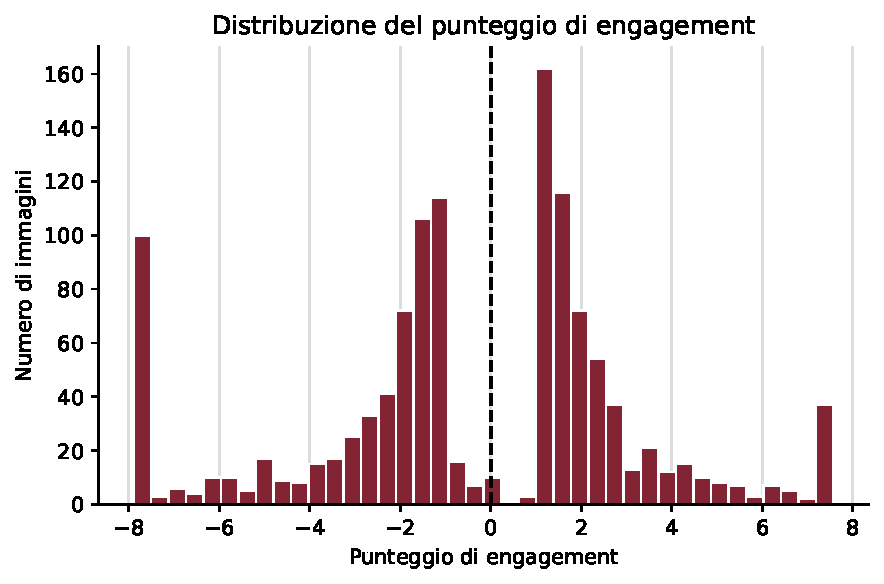
\includegraphics[width=0.7\textwidth]{engagement_istogramma.pdf}
    \caption{Istogramma del punteggio di engagement sulle 1.212 immagini selezionate. I 127 valori esterni alle soglie di Tukey~\cite{tukey1977exploratory} sono riportati sulle rispettive soglie e contribuiscono alle barre ai bordi. La linea tratteggiata indica lo zero.}
    \label{fig:dataset-istogramma}
\end{minipage}
\bigskip

\begin{figure}[htbp]
    \centering
    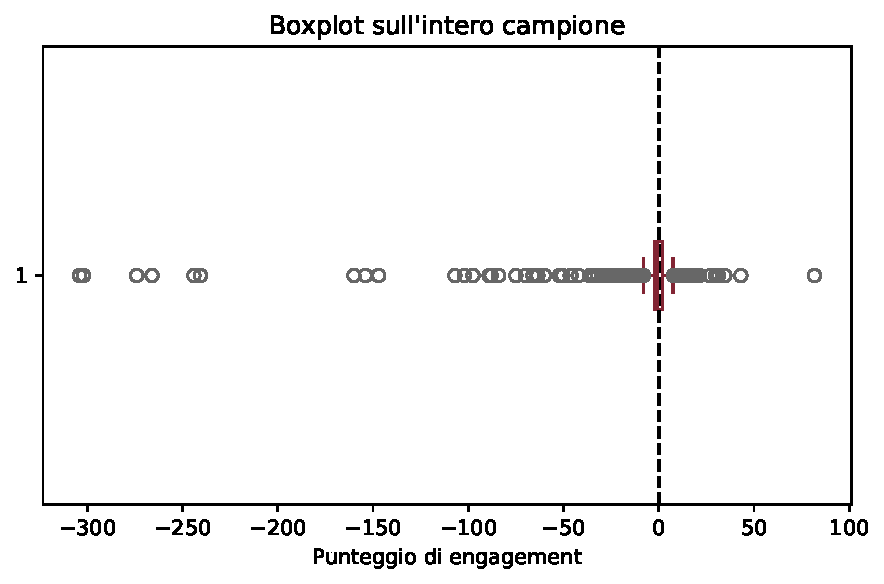
\includegraphics[width=0.7\textwidth]{engagement_boxplot.pdf}
    \caption{Box plot del punteggio di engagement sulle 1.212 immagini selezionate. La scatola rappresenta l'intervallo interquartile, la linea interna la mediana e i punti oltre i baffi i valori estremi~\cite{tukey1977exploratory}. La linea tratteggiata indica lo zero.}
    \label{fig:dataset-boxplot}
\end{figure}

\newpage
Dopo il filtraggio conto 584 score positivi, 618 negativi e 10 nulli. L'esclusione dell'intervallo $[-0{,}5;\,0{,}5]$ rimuove 16 osservazioni e lascia 1.196 esempi: 584 con prestazioni superiori alle aspettative e 612 con prestazioni inferiori. Applico la stessa regola alla tabella arricchita con le informazioni prodotte dalle elaborazioni successive, di 1.211 righe, e le osservazioni diventano 1.195, suddivise in 583 esempi con engagement superiore alle aspettative e 612 con engagement inferiore alle aspettative. Questa distinzione rende esplicita la differenza tra il campione descritto qui e quello riportato nelle analisi di classificazione archiviate.

\section{Limiti del dataset}
\label{sec:dataset-limiti}

La raccolta riguarda due piattaforme, 66 account in un intervallo di tre mesi. Questi confini delimitano il caso di studio. La prevalenza di Instagram, 68,2\% del totale dei post filtrati, e l'assenza di un protocollo completo di estrazione impediscono di considerare i dati selezionati una rappresentazione esaustiva dell'intera comunicazione politica online. L'estensione dei risultati ad altre campagne, periodi o ambiti del marketing richiede una verifica su nuove raccolte.

La scelta della prima immagine riduce ogni post a una sola componente visiva. La misura di engagement riguarda però il post nel suo complesso, che può includere testo e altri allegati. Le associazioni osservate coinvolgono quindi un contesto comunicativo che la rappresentazione dell'immagine descrive solo in parte.

Quando più post condividono il collegamento a un media, la selezione basata sull’indice di engagement privilegia per costruzione la prestazione più alta tra le occorrenze disponibili. Inoltre, il confronto degli identificatori dei file non elimina tutte le possibili ripetizioni visive. Queste due proprietà vanno considerate quando si interpreta la distribuzione della misura di engagement e quando si valuta l'indipendenza delle osservazioni.

Infine, l'engagement misura interazioni e non identifica direttamente consenso politico, persuasione o intenzione di voto. Il riferimento allo storico dell'account rapporta la misura alle sue prestazioni abituali, ma non permette di stabilire se una scelta visiva determina un cambiamento nelle interazioni. Utilizzo quindi il dataset per studiare le associazioni tra caratteristiche visive ed engagement e valutare quanto queste caratteristiche aiutano a prevederlo.

% !TeX root = ../tesi.tex
% !TeX encoding = UTF-8
% !TeX spellcheck = it_IT

\chapter{Localizzazione delle aree modificate e descrizione}
\label{chap:localizzazione-descrizione}

In questo capitolo descrivo come ricavo le regioni sospette dalle immagini selezionate e ne rappresento il contenuto mediante testo. Presento TruFor come componente esterno della pipeline (Sezione~\ref{sec:materiali-trufor}), poi il test preliminare su 100 immagini annotate (Sezione~\ref{sec:metodi-trufor-benchmark}) e l'applicazione al dataset filtrato (Sezione~\ref{sec:metodi-trufor-esecuzione}). Illustro quindi la creazione delle maschere e la loro valutazione (Sezione~\ref{sec:metodi-maschere}). Concludo con la descrizione tramite BLIP e OCR, i risultati ottenuti e gli esempi visivi (Sezione~\ref{sec:metodi-descrizioni}).

\section{TruFor come componente esterno}
\label{sec:materiali-trufor}

Utilizzo TruFor, descritto nel Capitolo~\ref{chap:background} e nel paper~\cite{Guillaro_2023_CVPR}. Clono il \href{https://github.com/grip-unina/TruFor}{repository ufficiale} nella cartella \path{TruFor/} del progetto. Mantengo separati il codice di TruFor e gli script delle elaborazioni successive. Uso il framework come componente a scatola nera: fornisco gli input e acquisisco gli output del modello. Mantengo i pesi preaddestrati durante tutte le elaborazioni.

Lo script \path{scripts/trufor.py} richiama \path{TruFor/TruFor_train_test/test.py}. La configurazione selezionata è \texttt{trufor\_ph3}; il file dei pesi è \path{TruFor/TruFor_train_test/weights/trufor_ph3/best.pth.tar}. Centralizzo i percorsi e i parametri di esecuzione in \path{scripts/config.py}.

La copia locale include modifiche per adattare l’esecuzione alle risorse del dispositivo: un limite massimo di pixel in ingresso e ottimizzazioni per il supporto della GPU. Descrivo il ridimensionamento dell'input nella Sezione~\ref{sec:metodi-trufor-esecuzione}. Questi interventi riguardano l'esecuzione del modello preaddestrato. 

Per aggiornare TruFor basta sostituire la cartella \path{TruFor/} con la nuova versione, riapplicare gli adattamenti per il dispositivo e adeguare gli script della pipeline alle eventuali variazioni dell’interfaccia e degli output.

\subsection{Organizzazione degli input e degli output}
\label{subsec:materiali-trufor-output}

Uso \path{scripts/temp/} come cartella di lavoro. Al suo interno, \path{images/} contiene i collegamenti ai file selezionati come input (Sottosezione~\ref{subsec:dataset-campione-filtrato}) e \path{npz/} contiene gli archivi prodotti da TruFor. Conservo i punteggi associati ai post in \path{dataset_filtered.csv}.

Per ogni file elaborato acquisisco un archivio NumPy, con estensione \texttt{.npz}. Il nome conserva quello dell'input e aggiunge l'estensione, per esempio \path{picture.jpg.npz}. Riporto nella Tabella~\ref{tab:materiali-trufor-output} i campi utilizzati dal progetto. Per il significato delle due mappe richiamo la Sottosezione~\ref{subsec:background-trufor-architettura}.

\begin{table}[htbp]
    \centering
    \small
    \caption{Campi degli output di TruFor utilizzati nella pipeline~\cite{Guillaro_2023_CVPR}.}
    \label{tab:materiali-trufor-output}
    \begin{tabular}{@{}lp{0.75\linewidth}@{}}
        \toprule
        Campo & Contenuto e utilizzo \\
        \midrule
        \texttt{map} & Mappa delle anomalie, usata per individuare le regioni sospette. \\
        \addlinespace
        \texttt{conf} & Mappa di confidenza, usata nell'elaborazione delle previsioni per pixel. \\
        \addlinespace
        \texttt{score} & Punteggio globale, riportato nella tabella del dataset come \texttt{trufor\_score}. \\
        \addlinespace
        \texttt{imgsize} & Altezza e larghezza originali, in pixel. \\
        \bottomrule
    \end{tabular}
\end{table}

Indico con $t_i$ il punteggio globale prodotto per l'immagine $i$ (Sottosezione~\ref{subsec:background-trufor-output}).

\section{Test preliminare di TruFor sul dataset}
\label{sec:metodi-trufor-benchmark}

\subsection{Annotazione manuale del campione}
\label{subsec:materiali-trufor-annotazioni}

Prima dell'elaborazione completa considero un sottoinsieme eterogeneo di 100 contenuti del dataset, scelti casualmente tra i post contenenti immagini. Assegno manualmente a ciascuno un'etichetta globale, che indico con $z_i$: 0 per i media che giudico autentici e 1 per quelli che credo alterati. Il campione comprende 38 casi nella prima classe e 62 nella seconda. Uso queste annotazioni come ground truth del confronto. Seguendo la convenzione definita nella Sottosezione~\ref{subsec:background-rilevamento-localizzazione}, considero positiva la classe ``alterato``, indipendentemente dal tipo di alterazione.

Registro le etichette in \path{scripts/temp/trufor_truth.csv}, con i campi \texttt{filename} e \texttt{label}. Il primo identifica il file senza estensione; il secondo contiene $z_i$.

Attribuisco alla verifica un carattere esplorativo. Le annotazioni riflettono il mio giudizio come unico annotatore e servono a esaminare il comportamento di TruFor sulla raccolta. Le etichette globali permettono di valutare il rilevamento; la valutazione della localizzazione richiede invece un riferimento per ciascun pixel.

\subsection{Protocollo di valutazione}
\label{subsec:trufor-test-protocollo}

Eseguo TruFor sul campione descritto nella Sottosezione~\ref{subsec:materiali-trufor-annotazioni}. Confronto la previsione del modello con il mio giudizio sull'autenticità di ciascun contenuto.

Per ricavare una decisione dal punteggio $t_i$, applico la soglia $\tau=0{,}25$, impostata tramite \texttt{TRUFOR\_THRESHOLD}. Indico con $\widehat{z}_i$ la classe prevista:
\begin{equation}
    \widehat{z}_i =
    \begin{cases}
        1 & \text{se } t_i > \tau, \\
        0 & \text{se } t_i \leq \tau.
    \end{cases}
    \label{eq:metodi-trufor-soglia}
\end{equation}
Uso questa soglia soltanto per la verifica del rilevamento. L'elaborazione delle mappe usa parametri distinti.

Calcolo la matrice di confusione tra $z_i$ e $\widehat{z}_i$, insieme ad accuratezza, precisione, richiamo e F1-score. Confronto l'accuratezza con quella ottenuta assegnando sempre la classe più frequente nel campione. Calcolo anche l’AUC (Area Under the Curve) direttamente dai punteggi, per valutare la capacità di distinguere i casi autentici da quelli alterati senza fissare un’unica soglia decisionale.

Affianco alla configurazione scelta un confronto delle soglie da $0{,}20$ a $0{,}50$, con passo $0{,}05$. Per ciascuna ricalcolo le metriche sullo stesso campione. Uso queste prove per un benchmark preliminare della soglia decisionale e interpreto le misure come risultati esplorativi sui casi annotati. Mantengo fissi i pesi del modello.

Salvo il confronto in \path{trufor_confusion_matrix.txt}. Il documento contiene anche gli identificatori dei falsi positivi e dei falsi negativi, con i rispettivi punteggi, per consentire l'ispezione dei singoli casi.

\subsection{Risultati del test e confronto delle soglie}
\label{subsec:trufor-test-risultati}

Riporto nella Tabella~\ref{tab:trufor-confusione} il confronto con le annotazioni manuali.

\begin{table}[htbp]
    \centering
    \small
    \caption{Matrice di confusione sui 100 casi annotati, con soglia $0{,}25$. Le righe indicano le mie annotazioni; le colonne indicano le previsioni di TruFor.}
    \label{tab:trufor-confusione}
    \begin{tabular}{@{}lrrr@{}}
        \toprule
        Annotazione manuale & Previsto autentico & Previsto alterato & Totale \\
        \midrule
        Autentico & 24 & 14 & 38 \\
        Alterato & 11 & 51 & 62 \\
        \midrule
        Totale & 35 & 65 & 100 \\
        \bottomrule
    \end{tabular}
\end{table}

La Tabella~\ref{tab:trufor-confronto-soglie} mostra il confronto tra le soglie. Tra i valori esaminati, $0{,}25$ produce l'accuratezza e l'F1-score maggiori. La soglia $0{,}20$ favorisce il richiamo, mentre $0{,}50$ produce la precisione maggiore.

\begin{table}[htbp]
    \centering
    \small
    \caption{Confronto delle soglie sullo stesso campione di 100 casi. Il grassetto evidenzia la configurazione usata nel benchmark.}
    \label{tab:trufor-confronto-soglie}
    \begin{tabular}{@{}rrrrr@{}}
        \toprule
        Soglia & Accuratezza & Precisione & Richiamo & F1-score \\
        \midrule
        $0{,}20$ & $72{,}00\%$ & $72{,}97\%$ & $87{,}10\%$ & $0{,}7941$ \\
        $\mathbf{0{,}25}$ & $\mathbf{75{,}00\%}$ & $\mathbf{78{,}46\%}$ & $\mathbf{82{,}26\%}$ & $\mathbf{0{,}8031}$ \\
        $0{,}30$ & $73{,}00\%$ & $79{,}66\%$ & $75{,}81\%$ & $0{,}7769$ \\
        $0{,}35$ & $70{,}00\%$ & $79{,}63\%$ & $69{,}35\%$ & $0{,}7414$ \\
        $0{,}40$ & $67{,}00\%$ & $80{,}85\%$ & $61{,}29\%$ & $0{,}6972$ \\
        $0{,}45$ & $62{,}00\%$ & $81{,}58\%$ & $50{,}00\%$ & $0{,}6200$ \\
        $0{,}50$ & $61{,}00\%$ & $82{,}86\%$ & $46{,}77\%$ & $0{,}5979$ \\
        \bottomrule
    \end{tabular}

    \medskip
    \begin{minipage}{0.9\linewidth}
        \small
        L'accuratezza del riferimento che assegna sempre la classe maggioritaria, ``alterato'', è pari al $62{,}00\%$. L'AUC è pari a $0{,}7538$ ed è calcolata dai punteggi continui, indipendentemente dalla soglia scelta.
    \end{minipage}
\end{table}

\section{Applicazione di TruFor al dataset filtrato}
\label{sec:metodi-trufor-esecuzione}

Dopo la verifica preliminare applico TruFor all'intero dataset filtrato. Lo script \path{scripts/trufor.py} avvia il programma di inferenza in un processo separato, usando l'interprete Python dell'ambiente corrente. Fornisco come argomenti le cartelle degli input e degli output e il limite di risoluzione.

Imposto \texttt{TRUFOR\_MAX\_PIXELS} a 6.000.000. Se un input supera il limite il caricatore lo ridimensiona mantenendo le proporzioni. Il modello esegue l'inferenza sul contenuto; il programma riporta poi le mappe alle dimensioni originali tramite interpolazione bilineare. Il punteggio globale deriva dall'input effettivamente elaborato.

Organizzo l'esecuzione in gruppi di 50 file e inserisco una pausa di 180 secondi tra gruppi consecutivi. Per ogni gruppo lo script prepara una cartella temporanea con i collegamenti agli originali da elaborare e avvia un nuovo processo. Il programma carica il modello una volta per gruppo ed elabora un file alla volta. Questa organizzazione regola il carico della macchina durante l'esecuzione.

Gli output vengono salvati in \path{scripts/temp/npz/}, un file \texttt{.npz} dopo ogni elaborazione completata. Se un gruppo si interrompe per un crash, restano disponibili i risultati dei gruppi precedenti e quelli già salvati del gruppo interrotto.

Per esecuzioni successive il programma salta gli input associati a output già presenti; posso quindi riprendere il lavoro dagli elementi mancanti. Il riuso degli output presuppone la stessa configurazione di elaborazione; un cambio di configurazione richiede di rigenerarli o salvarli in una cartella distinta.

Estraggo dagli archivi il campo \texttt{score}, descritto nella Tabella~\ref{tab:materiali-trufor-output}, e lo rinomino \texttt{trufor\_score}. Aggiorno la tabella \path{dataset_filtered.csv} tramite \texttt{filename}, ottenuto dal nome dell'output senza le estensioni. L'unione conserva solo le osservazioni con una corrispondenza. Mantengo le mappe negli archivi per i passaggi successivi della pipeline.

\section{Creazione e valutazione delle maschere}
\label{sec:metodi-maschere}

Uso \path{scripts/mask.py} per selezionare le regioni sospette da fornire alla successiva descrizione testuale. Uso le mappe di anomalia e confidenza salvate da TruFor nei file .npz, descritti nella Sottosezione~\ref{subsec:materiali-trufor-output}. Applico questo passaggio a tutte le immagini con output disponibile, indipendentemente dalla decisione sul punteggio globale $t_i$.

\subsection{Annotazioni delle regioni e maschere di riferimento}
\label{subsec:materiali-maschere-riferimento}

Per valutare la localizzazione delle maschere uso le stesse 100 immagini della Sottosezione~\ref{subsec:materiali-trufor-annotazioni}. Disegno manualmente una maschera per ciascuna immagine: coloro di bianco le regioni che credo alterate e di nero quelle autentiche. Conservo queste maschere di riferimento in \path{masked_truth/}, associandole agli originali tramite il nome del file.

Svolgo le due valutazioni in modo indipendente. L'etichetta $z_i$, definita nella Sottosezione~\ref{subsec:materiali-trufor-annotazioni}, esprime il mio parere sull'aspetto complessivo dell'immagine. La maschera registra il giudizio sulle singole regioni. Un contenuto classificato globalmente come autentico può quindi avere regioni annotate come alterate, anche per un totale di aree maggiore della metà della superficie. L'etichetta globale non deriva dalla percentuale di pixel bianchi.

La maschera binaria indica quali pixel conservare e quali escludere, secondo la segmentazione descritta nella Sottosezione~\ref{subsec:background-rilevamento-localizzazione}. Applicandola all'originale ottengo l'immagine mascherata, che mantiene i colori dei pixel selezionati e rende neri quelli esclusi.

Per misurare la sovrapposizione uso l'\emph{Intersection over Union} (IoU). Indico con $P_i$ l'insieme dei pixel previsti come alterati e con $T_i$ quello dei pixel alterati nel riferimento manuale:
\begin{equation}
    \operatorname{IoU}_i=\frac{|P_i\cap T_i|}{|P_i\cup T_i|}.
    \label{eq:maschere-iou}
\end{equation}
La misura vale 1 quando le regioni coincidono e 0 quando sono disgiunte. Se entrambi gli insiemi sono vuoti, adotto la convenzione $\operatorname{IoU}_i=1$. Calcolo la IoU sia aggregando le intersezioni e le unioni di tutte le immagini, sia facendo la media dei valori ottenuti per ciascuna immagine. Nel primo caso incidono maggiormente le immagini con regioni di unione più estese; nel secondo ogni immagine ha lo stesso peso.

\subsection{Dalle mappe all'immagine mascherata}
\label{subsec:metodi-maschere-creazione}

Uso le mappe di anomalia e confidenza già riportate alle dimensioni originali, come descritto nella Sezione~\ref{sec:metodi-trufor-esecuzione}. Nella maschera iniziale seleziono un pixel solo quando entrambi i valori raggiungono o superano le rispettive soglie, riportate nella Tabella~\ref{tab:metodi-maschere-parametri}.

Nelle immagini che combinano una fotografia e uno sfondo grafico uniforme, la maschera può selezionare la fotografia al posto della grafica. Per correggere questi casi introduco una regola di inversione della maschera. Uso il \emph{gradiente di Sobel}, che stima le variazioni locali di intensità in orizzontale ($g_x$) e in verticale ($g_y$) sull'immagine in scala di grigi~\cite{996}. Considero \emph{piatti} i pixel per cui il modulo $\sqrt{g_x^2+g_y^2}$ è inferiore alla soglia configurata. Inverto la maschera se la frazione di pixel piatti all'esterno supera quella all'interno della selezione di almeno il margine previsto. Applico la regola solo se la regione selezionata raggiunge l'area minima e lascia una parte dell'immagine esclusa. L'uniformità è però solo un indizio: la regola può invertire la selezione anche in presenza di sfondi autentici uniformi. I valori della configurazione sono specificati nella Tabella~\ref{tab:metodi-maschere-parametri}.

Applico quindi una pulizia morfologica con un elemento strutturante ellittico. Eseguo prima l'\emph{apertura}, cioè erosione seguita da dilatazione, per rimuovere piccoli elementi isolati. Eseguo poi la \emph{chiusura}, cioè dilatazione seguita da erosione, per colmare piccoli vuoti. Infine individuo le componenti connesse considerando gli otto vicini di ciascun pixel e scarto quelle con area inferiore alla frazione minima dell'immagine. Ottengo così la maschera finale. L'inversione e la pulizia possono includere anche pixel esclusi dalle soglie iniziali.

Applico la maschera finale all'originale secondo la definizione della Sottosezione~\ref{subsec:materiali-maschere-riferimento}. Salvo l'immagine mascherata in \path{scripts/temp/masked/}, in formato PNG senza perdita. Conservo anche gli output interamente neri, che indicano l'assenza di contenuto visibile dopo la selezione.

\subsection{Taratura dei parametri e valutazione}
\label{subsec:metodi-maschere-taratura}

Svolgo diverse iterazioni di test sul campione della Sottosezione~\ref{subsec:materiali-maschere-riferimento} per scegliere la configurazione da adottare. Valuto le configurazioni sulla base della matrice di confusione a livello di pixel. Sommo i conteggi di tutte le immagini e calcolo accuratezza, precisione, richiamo e F1-score. Aggiungo le misure di IoU definite nella stessa sottosezione.

Ricavo la previsione dalle immagini mascherate salvate, considerando positivo un pixel se almeno un canale ha intensità maggiore di zero. Confronto le prestazioni con una baseline che classifica tutti i pixel come alterati, per valutare la selezione rispetto alla conservazione dell'intera immagine.

Riporto nella Tabella~\ref{tab:metodi-maschere-parametri} la configurazione finale, registrata in \path{scripts/config.py}. Salvo le metriche e le IoU delle singole immagini nel report \path{mask_confusion_matrix.txt}; ne presento i risultati nella Sottosezione~\ref{subsec:risultati-maschere}.

\begin{table}[htbp]
    \centering
    \small
    \caption{Configurazione adottata per la creazione delle maschere. Le aree sono espresse rispetto alla superficie dell'immagine.}
    \label{tab:metodi-maschere-parametri}
    \begin{tabular}{@{}lr@{}}
        \toprule
        Parametro & Valore \\
        \midrule
        Soglia di anomalia & $0{,}50$ \\
        Soglia di confidenza & $0{,}30$ \\
        Inversione della polarità & Attiva \\
        Soglia del gradiente per i pixel piatti & $12$ \\
        Margine tra le frazioni di pixel piatti & $0{,}25$ \\
        Area minima per valutare l'inversione & $3\%$ \\
        Dimensione dell'elemento morfologico & $9\times9$ pixel \\
        Area minima delle componenti connesse & $0{,}2\%$ \\
        \bottomrule
    \end{tabular}
\end{table}

\subsection{Risultati della valutazione delle maschere}
\label{subsec:risultati-maschere}

Applico il protocollo della Sottosezione~\ref{subsec:metodi-maschere-taratura} alle 100 immagini annotate. Il report \path{mask_confusion_matrix.txt} comprende 148.230.685 pixel, dei quali il $66{,}29\%$ è annotato come alterato. Riporto nella Tabella~\ref{tab:risultati-maschere-confusione} i conteggi ottenuti con la configurazione finale.

\begin{table}[htbp]
    \centering
    \small
    \caption{Matrice di confusione a livello di pixel sulle immagini annotate manualmente.}
    \label{tab:risultati-maschere-confusione}
    \begin{tabular}{@{}lrr@{}}
        \toprule
        Annotazione manuale & Previsto autentico & Previsto alterato \\
        \midrule
        Autentico & 39.043.111 & 10.926.896 \\
        Alterato & 59.256.116 & 39.004.562 \\
        \bottomrule
    \end{tabular}
\end{table}

\begin{table}
    \centering
    \small
    \caption{Prestazioni della pipeline e della baseline che seleziona tutti i pixel. Fonte: \texttt{mask\_confusion\_matrix.txt}}
    \label{tab:risultati-maschere-metriche}
    \begin{tabular}{@{}lrr@{}}
        \toprule
        Metrica & Pipeline & Baseline \\
        \midrule
        Accuratezza & $52{,}65\%$ & $66{,}29\%$ \\
        Precisione & $78{,}12\%$ & $66{,}29\%$ \\
        Richiamo & $39{,}69\%$ & $100{,}00\%$ \\
        F1-score & $0{,}5264$ & $0{,}7973$ \\
        IoU aggregata & $0{,}3572$ & $0{,}6629$ \\
        IoU media & $0{,}3501$ & $0{,}6351$ \\
        \bottomrule
    \end{tabular}
\end{table}

\newpage
La Tabella~\ref{tab:risultati-maschere-metriche} mostra una precisione superiore alla baseline: tra i pixel conservati aumenta la quota che coincide con il riferimento alterato. Il richiamo indica però che recupero meno della metà dei pixel annotati come alterati. Ottengo valori di accuratezza, F1-score, IoU aggregata e IoU media inferiori a quelli della baseline che seleziona l'intera immagine. La quota elevata di pixel positivi nel riferimento favorisce questa baseline.

Uso il mascheramento per isolare il contenuto da descrivere, cercando di conservare dettagli e contesto utili. Una selezione troppo restrittiva può impoverire le descrizioni: l'utilità delle maschere va quindi valutata anche nei passaggi successivi della pipeline.

\newpage
\subsection{Esempi visivi su immagini pubbliche}
\label{subsec:risultati-maschere-esempi}

Per mostrare gli effetti del mascheramento elaboro quattro immagini senza copyright raccolte da \href{https://commons.wikimedia.org/wiki/Main_Page}{Wikimedia Commons}. Applico la stessa configurazione della pipeline e confronto gli input con le immagini mascherate nella Figura~\ref{fig:maschere-esempi}.

\bigskip\noindent
\begin{minipage}{\linewidth}
    \captionsetup{type=figure}
    \centering
    \renewcommand{\thesubfigure}{\Alph{subfigure}}
    \captionsetup[subfigure]{labelformat=simple,labelsep=period,hypcap=true}
    \makebox[0.48\linewidth]{\small Prima del mascheramento}\hfill
    \makebox[0.48\linewidth]{\small Dopo il mascheramento}\par\medskip
    \begin{subfigure}{\linewidth}
        \centering
        \makebox[0.48\linewidth]{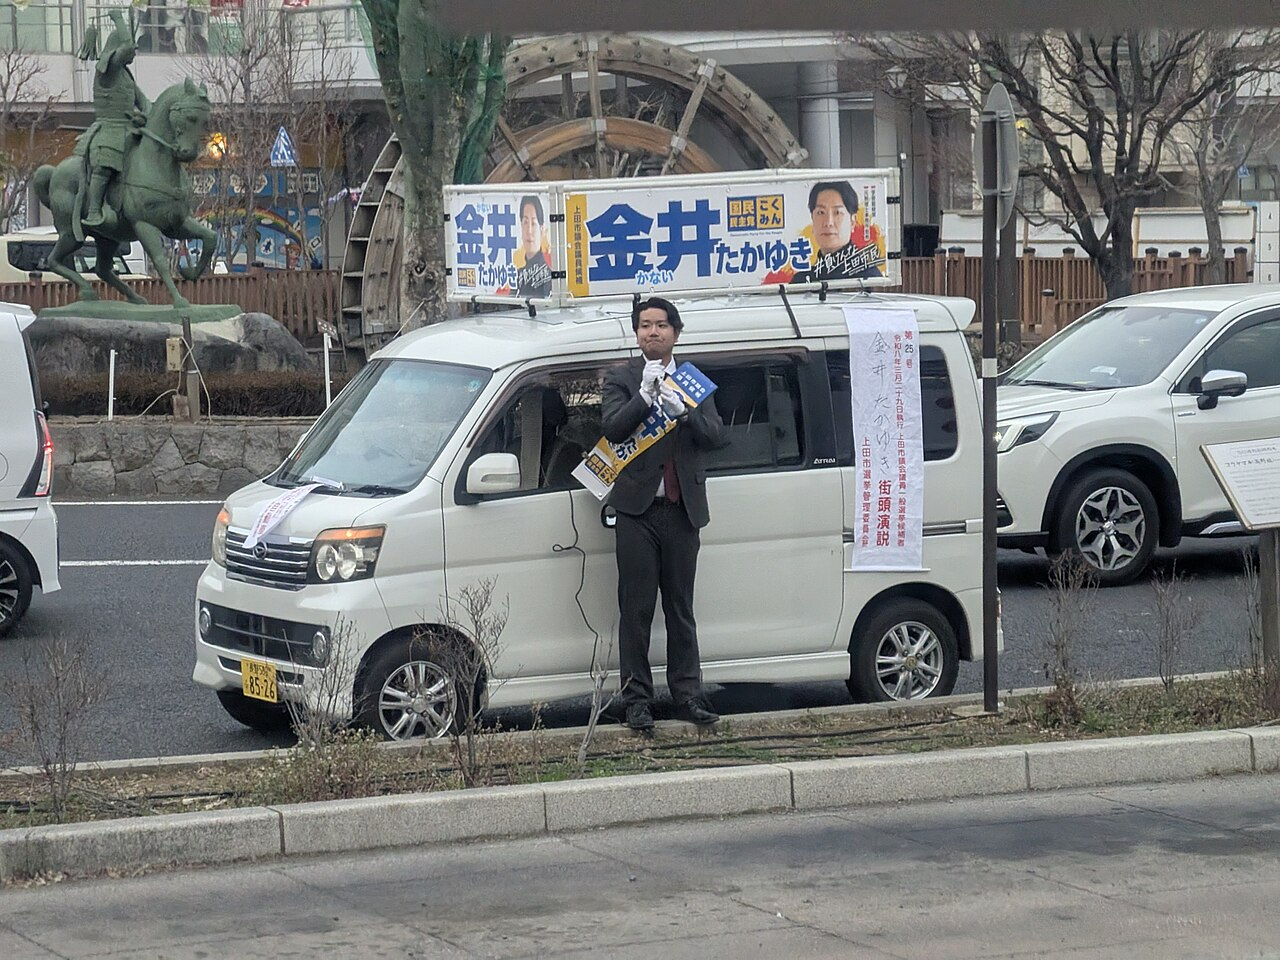
\includegraphics[width=0.48\linewidth,height=3.5cm,keepaspectratio]{Politician_in_front_of_Ueda_station.jpg}}\hfill
        \makebox[0.48\linewidth]{
\includegraphics[width=0.48\linewidth,height=3.5cm,keepaspectratio]{Politician_in_front_of_Ueda_station_masked.png}}
        \caption{Scena davanti alla stazione di Ueda. TruFor: $0{,}0156$; pixel non neri: $0{,}00\%$.}
        \label{fig:maschere-esempio-ueda}
    \end{subfigure}
    \par\medskip
    \begin{subfigure}{\linewidth}
        \centering
        \makebox[0.48\linewidth]{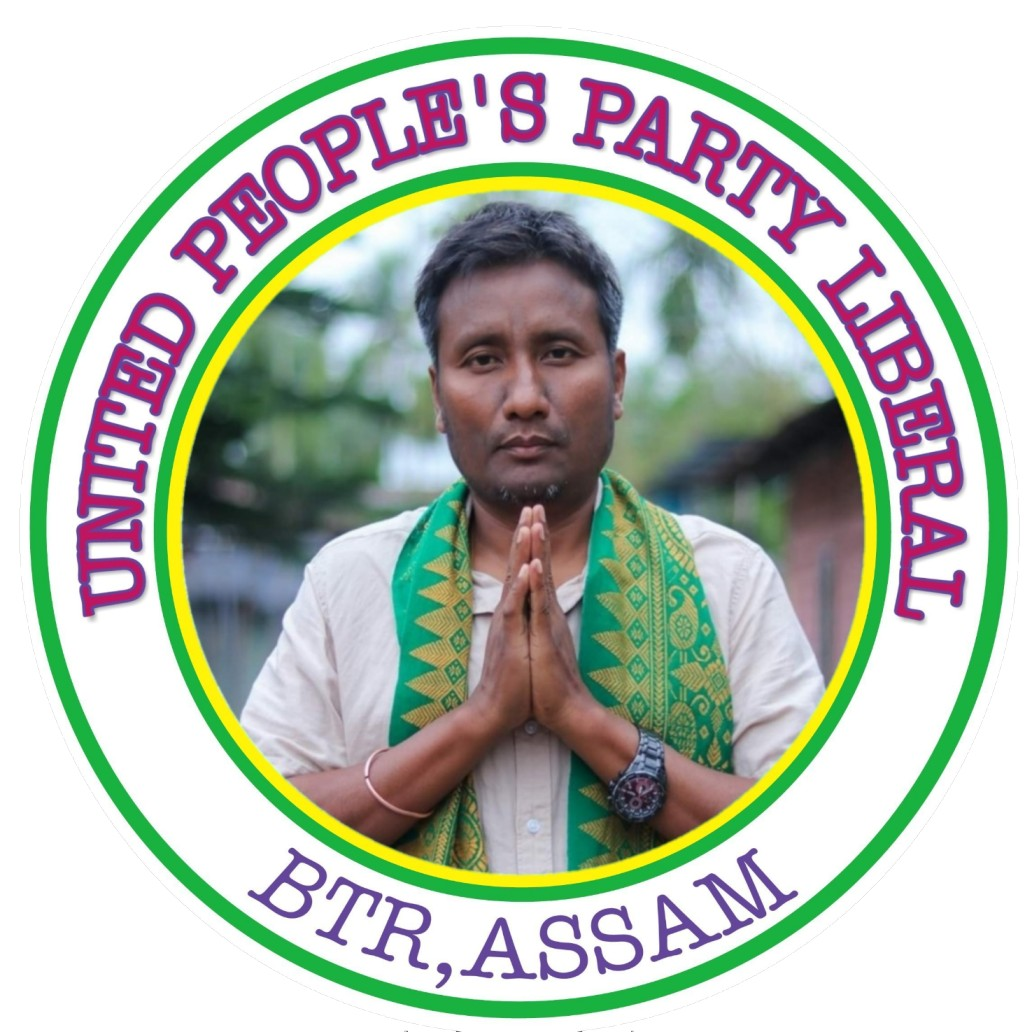
\includegraphics[width=0.48\linewidth,height=3.5cm,keepaspectratio]{Rakesh_Brahma,_EM_Bodoland_Territorial_Region.jpg}}\hfill
        \makebox[0.48\linewidth]{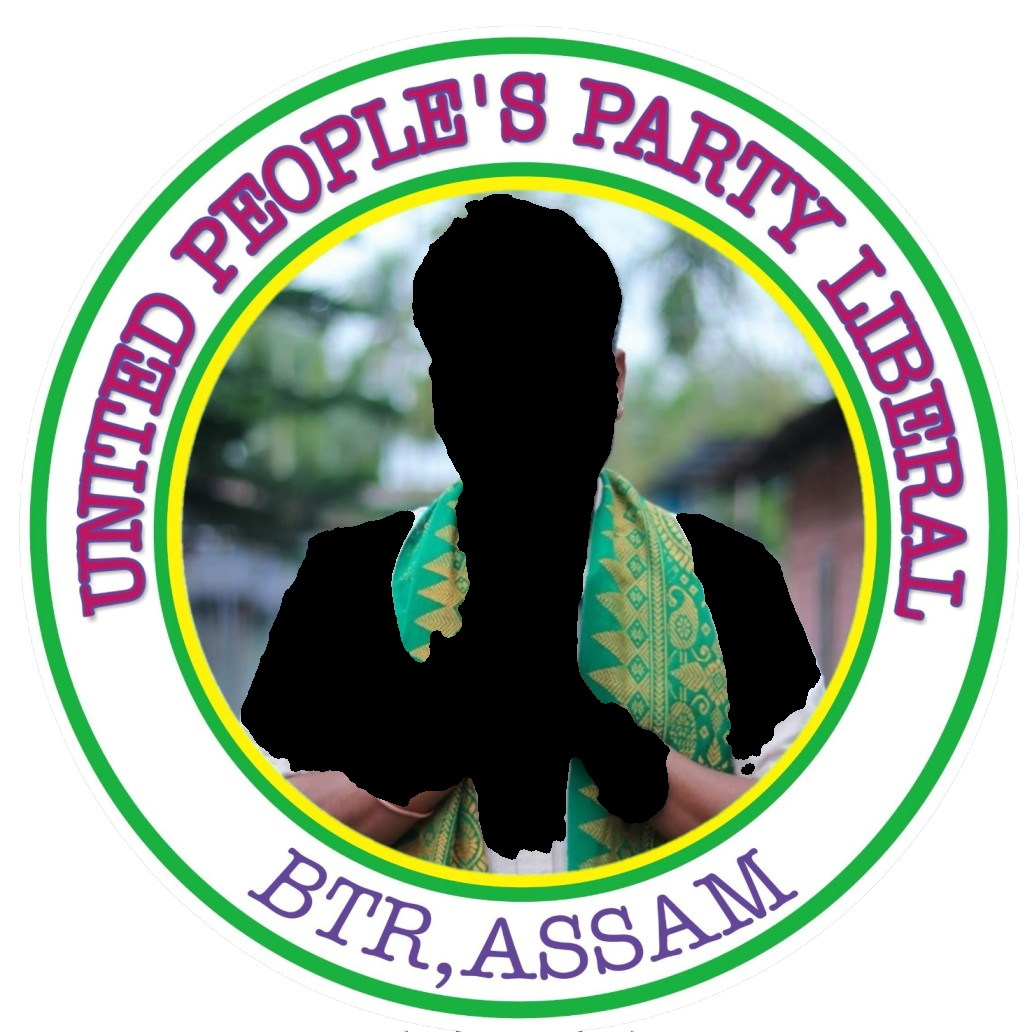
\includegraphics[width=0.48\linewidth,height=3.5cm,keepaspectratio]{Rakesh_Brahma,_EM_Bodoland_Territorial_Region_masked.png}}
        \caption{Ritratto con cornice grafica. TruFor: $0{,}9043$; pixel non neri: $85{,}09\%$.}
        \label{fig:maschere-esempio-brahma}
    \end{subfigure}
    \par\medskip
    \begin{subfigure}{\linewidth}
        \centering
        \makebox[0.48\linewidth]{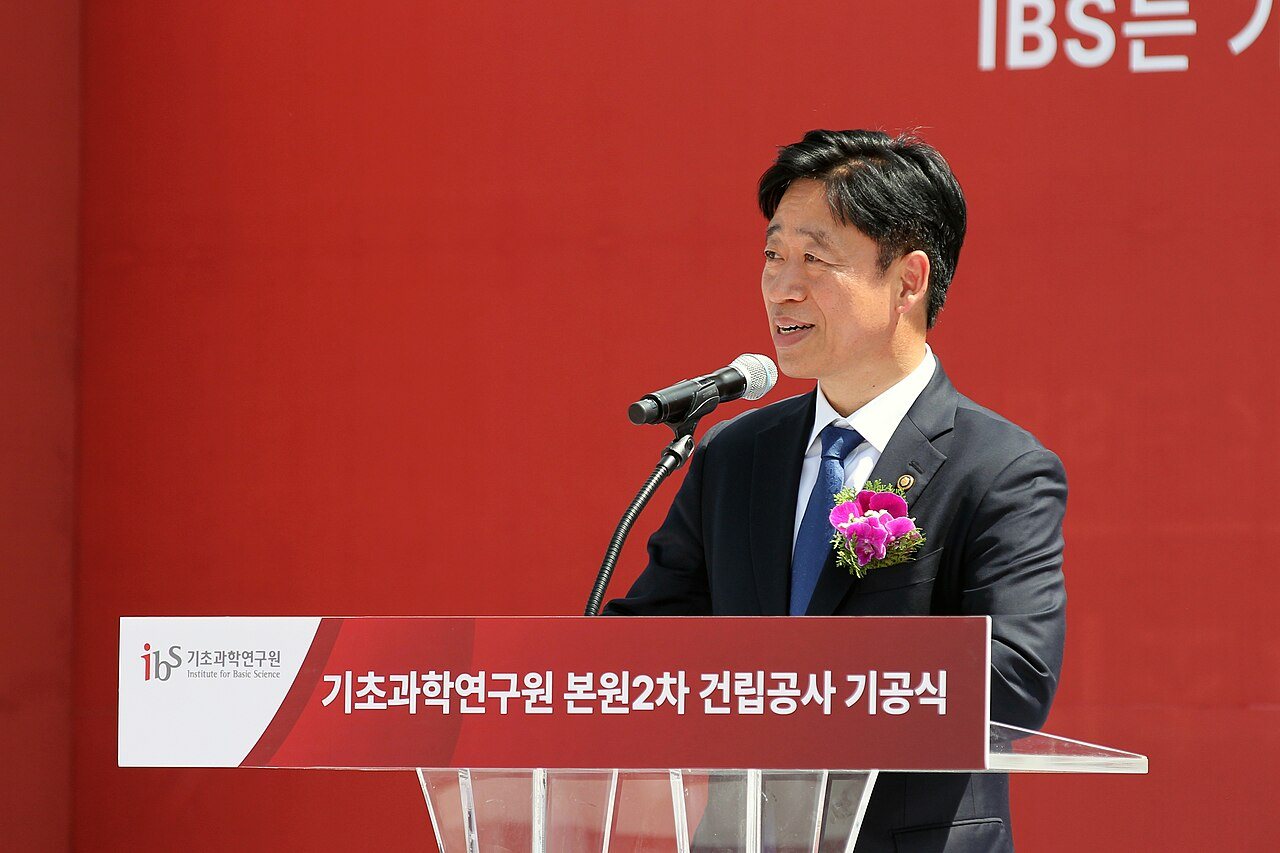
\includegraphics[width=0.48\linewidth,height=3.5cm,keepaspectratio]{South_Korean_politician_조승래.jpg}}\hfill
        \makebox[0.48\linewidth]{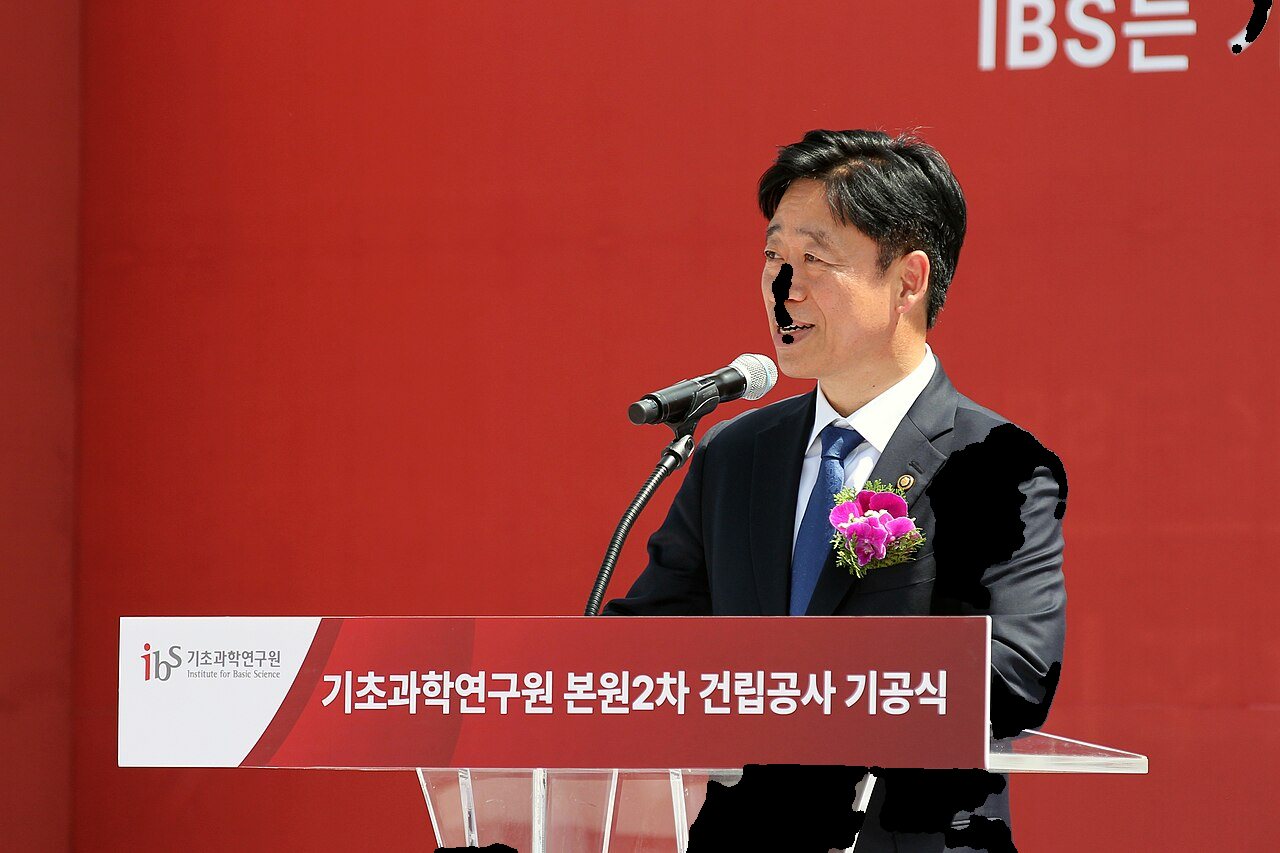
\includegraphics[width=0.48\linewidth,height=3.5cm,keepaspectratio]{South_Korean_politician_조승래_masked.png}}
        \caption{Discorso al podio. TruFor: $0{,}1124$; pixel non neri: $96{,}27\%$.}
        \label{fig:maschere-esempio-podio}
    \end{subfigure}
    \par\medskip
    \begin{subfigure}{\linewidth}
        \centering
        \makebox[0.48\linewidth]{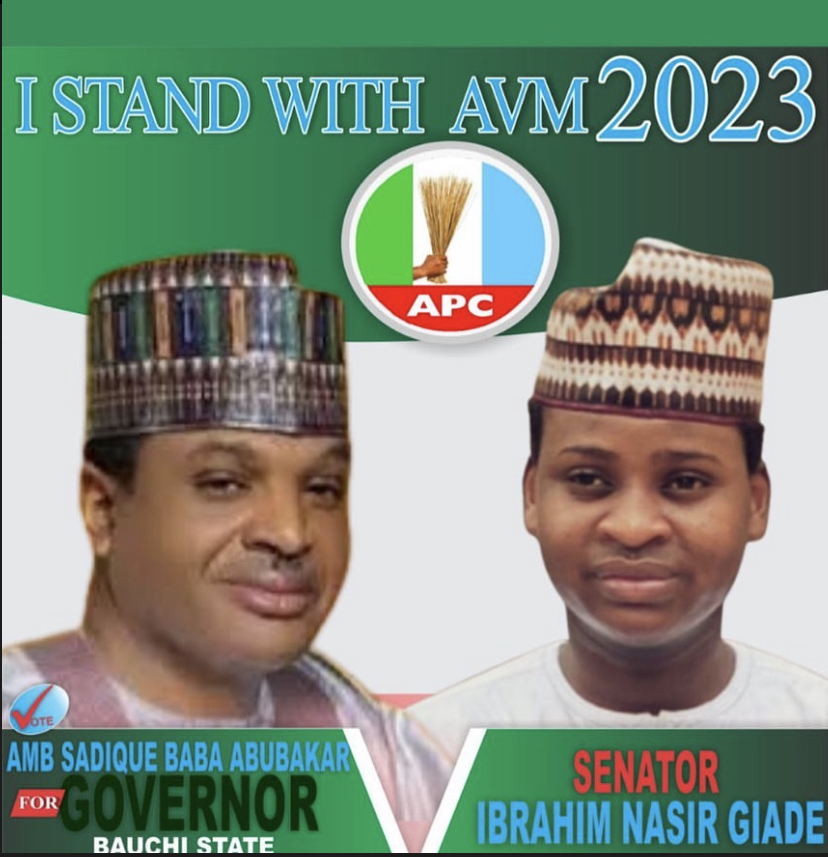
\includegraphics[width=0.48\linewidth,height=3.5cm,keepaspectratio]{Young_Politician_Naseer_Giade.jpg}}\hfill
        \makebox[0.48\linewidth]{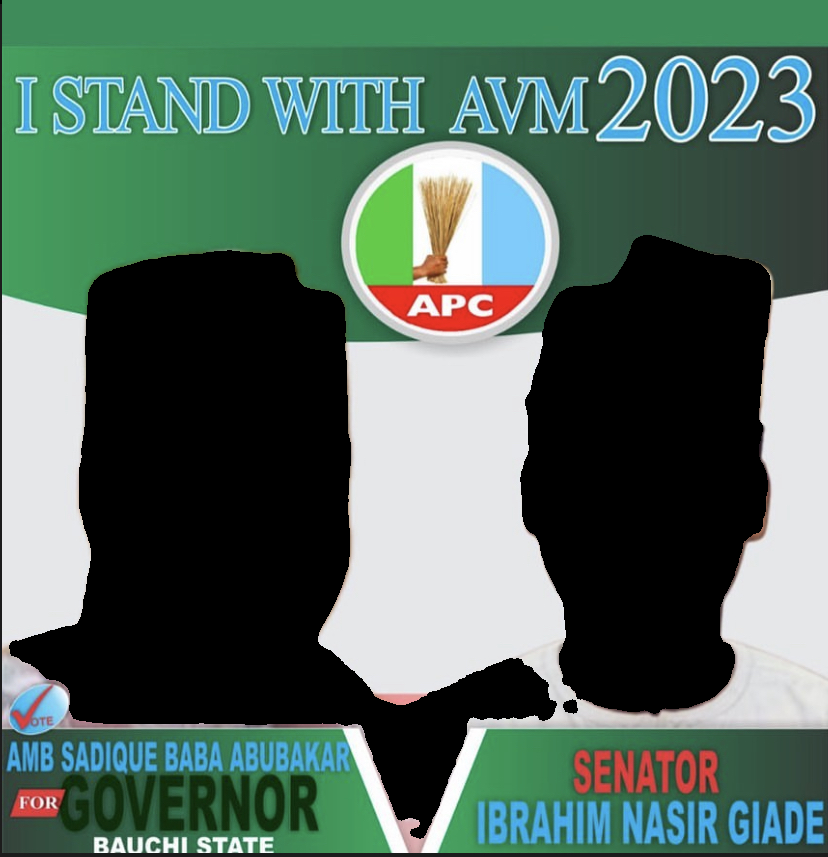
\includegraphics[width=0.48\linewidth,height=3.5cm,keepaspectratio]{Young_Politician_Naseer_Giade_masked.png}}
        \caption{Manifesto elettorale. TruFor: $0{,}9307$; pixel non neri: $67{,}43\%$.}
        \label{fig:maschere-esempio-manifesto}
    \end{subfigure}
    \caption[Mascheramento dei quattro esempi]{Mascheramento dei quattro esempi. I pixel neri indicano le regioni escluse. Fonti: \subref{fig:maschere-esempio-ueda}, \href{https://commons.wikimedia.org/wiki/File:Politician_in_front_of_Ueda_station.jpg}{Syced}; \subref{fig:maschere-esempio-brahma}, \href{https://commons.wikimedia.org/wiki/File:Rakesh_Brahma,_EM_Bodoland_Territorial_Region.jpg}{Swrang Borgoary}; \subref{fig:maschere-esempio-podio}, \href{https://commons.wikimedia.org/wiki/File:South_Korean_politician_조승래.jpg}{Rickinasia}; \subref{fig:maschere-esempio-manifesto}, \href{https://commons.wikimedia.org/wiki/File:Young_Politician_Naseer_Giade.jpg}{Naseer001}.}
    \label{fig:maschere-esempi}
\end{minipage}
\bigskip

\section{Descrizione testuale delle regioni sospette}
\label{sec:metodi-descrizioni}

Con \path{scripts/describe.py} trasformo le immagini mascherate nel campo \texttt{anomaly\_txt}, definito nella Sottosezione~\ref{subsec:materiali-descrizioni}. Uso BLIP per descrivere il contenuto visivo e EasyOCR per estrarre le scritte. La Figura~\ref{fig:descrizione-flusso} riassume il percorso degli input che superano il controllo sull'area visibile.

\begin{figure}[htbp]
    \centering
    \begin{tikzpicture}[
        box/.style={draw, rounded corners, align=center, font=\small, minimum height=1cm, text width=2.1cm},
        flow/.style={-{Latex}, thick}
    ]
        \node[box] (input) at (0,0) {Immagine\\mascherata};
        \node[box] (crop) at (2.9,0) {Ritaglio del\\contenuto visibile};
        \node[box] (blip) at (5.8,0.9) {BLIP\\Didascalia};
        \node[box] (ocr) at (5.8,-0.9) {EasyOCR\\Parole lette};
        \node[box, text width=2.7cm] (text) at (9,0) {Normalizzazione\\e unione};
        \draw[flow] (input) -- (crop);
        \draw[flow] (crop.east) -- (blip.west);
        \draw[flow] (crop.east) -- (ocr.west);
        \draw[flow] (blip.east) -- (text.west);
        \draw[flow] (ocr.east) -- (text.west);
    \end{tikzpicture}
    \caption{Costruzione della descrizione per le immagini con più del $2\%$ di pixel non neri. BLIP e OCR ricevono lo stesso ritaglio; normalizzo e unisco i rispettivi output nel campo \texttt{anomaly\_txt}.}
    \label{fig:descrizione-flusso}
\end{figure}

\subsection{Modelli e formato della descrizione}
\label{subsec:materiali-descrizioni}

Per descrivere le regioni sospette uso le immagini a colori su sfondo nero prodotte dal mascheramento automatico e salvate in \path{scripts/temp/masked/}.

Per BLIP~\cite{pmlr-v162-li22n}, descritto nella Sottosezione~\ref{subsec:background-blip}, adotto il modello \texttt{Salesforce/blip-image-captioning-large}, distribuito su \href{https://huggingface.co/Salesforce/blip-image-captioning-large}{Hugging Face}. Lo carico attraverso le classi \texttt{BlipProcessor} e \texttt{BlipForConditionalGeneration} della libreria Transformers~\cite{wolf-etal-2020-transformers}. Il processore prepara le immagini per la rete e converte i token generati in testo. Fornisco soltanto l'immagine, senza un testo iniziale che orienti la didascalia.

Per l'OCR uso EasyOCR~\cite{easyocr_software}, specificato nella Sottosezione~\ref{subsec:background-ocr}, con le lingue italiano e inglese. Con questa combinazione, il lettore predefinito carica il rilevatore CRAFT e il riconoscitore \texttt{latin\_g2}, basato sull'architettura CRNN. Mantengo i pesi distribuiti per entrambi gli strumenti, senza un ulteriore addestramento sul dataset politico.

Raccolgo il risultato nel campo \texttt{anomaly\_txt} di \path{dataset_filtered.csv}, associato a ciascuna immagine tramite \texttt{filename}. Il campo contiene la didascalia inglese normalizzata, seguita dalle parole riconosciute dall'OCR, oppure l'etichetta convenzionale \texttt{nomask}. Quest'ultima segnala l'assenza di una descrizione utilizzabile secondo il controllo dell'area visibile (Sottosezione~\ref{subsec:metodi-descrizioni-input}) e la normalizzazione del testo (Sottosezione~\ref{subsec:metodi-descrizioni-output}).

La rappresentazione può mescolare inglese e italiano e serve come input per la successiva analisi testuale.

\subsection{Controllo dell'area visibile e ritaglio}
\label{subsec:metodi-descrizioni-input}

Prima di interrogare i modelli misuro la frazione di pixel non neri nell'immagine mascherata. Se questa frazione non supera la soglia indicata nella Tabella~\ref{tab:descrizioni-parametri}, assegno \texttt{nomask} e salto sia BLIP sia l'OCR, per evitare la generazione di testo da input con contenuto visibile assente o limitato. Questa condizione può verificarsi anche per regioni selezionate piccole o contenenti pixel originariamente neri, indistinguibili dallo sfondo del mascheramento. L'etichetta \texttt{nomask} indica quindi l'esclusione dalla descrizione, non l'autenticità dell'immagine.

Per le altre immagini ritaglio il rettangolo che racchiude tutti i pixel non neri, aggiungendo un margine entro i bordi dell'immagine. Fornisco lo stesso ritaglio a BLIP ed EasyOCR, riducendo la cornice nera intorno al contenuto. Le aree nere interne rimangono tali e le eventuali regioni separate vengono descritte insieme.

\subsection{Generazione della didascalia e lettura delle scritte}
\label{subsec:metodi-descrizioni-modelli}

Elaboro le immagini in gruppi e carico i modelli una sola volta per esecuzione. Salto i file illeggibili. Riporto nella Tabella~\ref{tab:descrizioni-parametri} i parametri della configurazione corrente, definiti in \path{scripts/config.py}.

Uso BLIP in precisione a 32 bit, selezionando nell'ordine NVIDIA CUDA, Apple MPS o la CPU secondo la disponibilità. Per generare le didascalie uso la \emph{beam search}: a ogni passo seleziono più sequenze candidate e restituisco quella con il punteggio finale migliore.

Per controllare la lunghezza della didascalia generata da BLIP, imposto un numero minimo e massimo di nuovi token per immagine. Penalizzo il riuso dei token già presenti e impedisco la ripetizione di sequenze di lunghezza prefissata. Mantengo disattivato il campionamento casuale. I parametri di temperatura, selezione probabilistica e seme casuale previsti per la modalità alternativa restano quindi inattivi. Queste impostazioni agiscono durante la generazione, prima della normalizzazione del testo e dell'aggiunta delle parole riconosciute dall'OCR.

Configuro EasyOCR per eseguire i calcoli sulla GPU, quando disponibile, così da velocizzare il riconoscimento delle scritte. In assenza di una GPU compatibile, il programma usa la CPU. Richiedo un ingrandimento prima del rilevamento, per favorire la localizzazione delle scritte piccole. Conservo le trascrizioni che raggiungono la soglia di confidenza, le normalizzo come descritto nella Sottosezione~\ref{subsec:metodi-descrizioni-output} e scarto le parole che non raggiungono la lunghezza minima prevista. Ordino le parole candidate per confidenza decrescente del rispettivo riquadro, elimino i duplicati e ne limito il numero. L'ordine delle parole nell'immagine non è conservato. Questo limite riduce il peso delle immagini dense di testo. Se l'OCR fallisce su una singola immagine, mantengo la sola didascalia di BLIP.

Salvo le descrizioni di ogni gruppo completato in \path{description_temp.csv}. In caso di interruzione, riparto saltando i file già registrati. La ripresa presuppone che modelli, maschere e parametri restino gli stessi.

Al termine unisco le descrizioni a \path{dataset_filtered.csv} tramite \texttt{filename}, conservando solo le osservazioni corrispondenti e prive di valori mancanti. Rimuovo quindi il file intermedio.

\begin{table}[htbp]
    \centering
    \small
    \caption{Parametri per la descrizione delle immagini mascherate. La lunghezza BLIP è espressa in token; i limiti OCR riguardano le parole dopo la normalizzazione~\cite{pmlr-v162-li22n, easyocr_software}.}
    \label{tab:descrizioni-parametri}
    \begin{tabular}{@{}llr@{}}
        \toprule
        Componente & Parametro & Valore \\
        \midrule
        Input & Soglia di pixel non neri per \texttt{nomask} & $\leq 2\%$ \\
              & Ritaglio al rettangolo non nero & Attivo \\
              & Margine del ritaglio & 10 pixel \\
        \addlinespace
        BLIP & Sequenze candidate nella beam search & 5 \\
             & Nuovi token, minimo-massimo & 5--40 \\
             & Penalità di ripetizione & $1{,}3$ \\
             & Lunghezza delle sequenze non ripetibili & 2 token \\
             & Campionamento casuale & Disattivato \\
             & Rimozione delle parole duplicate & Attiva \\
        \addlinespace
        OCR & Lingue & Italiano, inglese \\
            & Fattore di ingrandimento richiesto & $1{,}5$ \\
            & Confidenza minima del riquadro & $0{,}65$ \\
            & Lunghezza minima delle parole & 3 lettere \\
            & Numero massimo di parole distinte & 20 \\
        \addlinespace
        Esecuzione & Immagini per gruppo & 30 \\
        \bottomrule
    \end{tabular}
\end{table}

\newpage
\subsection{Normalizzazione e unione del testo}
\label{subsec:metodi-descrizioni-output}

Applico la funzione \texttt{clean\_text} separatamente alla didascalia di BLIP e alle trascrizioni di EasyOCR. Riconduco le lettere accentate alla forma senza accento, converto il testo in minuscolo e sostituisco ogni carattere diverso da \texttt{a--z} con uno spazio. Nella didascalia mantengo solo la prima occorrenza di ciascuna parola; nell'OCR elimino i duplicati durante la selezione per confidenza. Concateno infine i due contributi. Una parola presente in entrambi può quindi comparire due volte nel risultato. Se la stringa finale è vuota, assegno \texttt{nomask}.

Queste scelte preparano il testo per un'analisi lessicale. Rimuovendo le cifre, perdo informazioni come anni e i numeri presenti nelle date; il limite minimo OCR esclude anche sigle di due lettere. Conservo in questa fase articoli e preposizioni. La rimozione delle parole funzionali, o \emph{stop word}, si effettua nella successiva vettorizzazione.

\subsection{Controllo delle descrizioni e limiti}
\label{subsec:metodi-descrizioni-controllo}

Produco \path{description_report.txt} con il numero di risultati, il conteggio di \texttt{nomask}, la lunghezza minima, mediana e massima e le dieci parole più frequenti. Riporto i valori nella Sottosezione~\ref{subsec:risultati-descrizioni}. Calcolo lunghezze e frequenze soltanto sulle descrizioni diverse da \texttt{nomask}, dopo l'unione di BLIP e OCR. Queste statistiche permettono di controllare la copertura e la distribuzione del testo prodotto. Per misurarne la correttezza servirebbero didascalie e trascrizioni di riferimento, distinte dalle annotazioni forensi.

La descrizione eredita i limiti della maschera: parti escluse possono interrompere parole o rimuovere il contesto necessario a interpretare un oggetto. BLIP può generare dettagli assenti, cioè \emph{allucinazioni}, oppure descrivere lo sfondo nero introdotto dalla procedura. Anche l'OCR può produrre letture errate dopo il filtraggio. Considero quindi \texttt{anomaly\_txt} una rappresentazione da valutare nelle analisi successive, anziché una verifica delle manipolazioni.

Mostro gli effetti del mascheramento nella Sottosezione~\ref{subsec:risultati-maschere-esempi} e le descrizioni ottenute nella Sottosezione~\ref{subsec:risultati-descrizioni-esempi}. Illustro la perdita di contesto, gli errori nel testo e l'interpretazione delle aree nere introdotte dalla maschera.

\subsection{Risultati delle descrizioni sul dataset}
\label{subsec:risultati-descrizioni}

Riporto nella Tabella~\ref{tab:risultati-descrizioni} i risultati del report \path{description_report.txt}, prodotto con la procedura della Sezione~\ref{sec:metodi-descrizioni}. Su 1.211 immagini ottengo 898 descrizioni testuali ($74{,}15\%$) e 313 etichette \texttt{nomask} ($25{,}85\%$).

\begin{table}[htbp]
    \centering
    \small
    \caption{Riepilogo delle descrizioni e dieci parole più frequenti, da \texttt{description\_report.txt}. Lunghezze e frequenze escludono \texttt{nomask}.}
    \label{tab:risultati-descrizioni}
    \begin{tabular}{@{}lr@{}}
        \toprule
        Misura & Valore \\
        \midrule
        Immagini con risultato archiviato & 1.211 \\
        Etichette \texttt{nomask} & 313 \\
        Lunghezza minima & 5 parole \\
        Lunghezza mediana & 17 parole \\
        Lunghezza massima & 36 parole \\
        \midrule
        Parola & Occorrenze \\
        \midrule
        \texttt{a} & 865 \\
        \texttt{is} & 727 \\
        \texttt{of} & 666 \\
        \texttt{there} & 659 \\
        \texttt{in} & 415 \\
        \texttt{man} & 401 \\
        \texttt{with} & 395 \\
        \texttt{and} & 309 \\
        \texttt{picture} & 246 \\
        \texttt{poster} & 199 \\
        \bottomrule
    \end{tabular}
\end{table}

La quota di \texttt{nomask} va interpretata secondo le condizioni definite nelle Sottosezioni~\ref{subsec:metodi-descrizioni-input} e~\ref{subsec:metodi-descrizioni-output}.

Le lunghezze contano le parole dopo la normalizzazione e l'unione di BLIP e OCR, quindi hanno un significato diverso dal limite di 5--40 token imposto alla generazione BLIP. Tra i termini più frequenti prevalgono parole funzionali inglesi e compaiono anche \texttt{man}, \texttt{picture} e \texttt{poster}.

Le descrizioni ottenute sono disponibili per la successiva analisi dell'engagement. Le statistiche ne descrivono la copertura e la composizione, ma non misurano la correttezza delle didascalie o delle trascrizioni. Il campo finale unisce i due contributi e non permette di valutarli separatamente.

\subsection{Descrizioni degli esempi visivi}
\label{subsec:risultati-descrizioni-esempi}

Nella Tabella~\ref{tab:descrizioni-esempi-commons} riporto il campo \texttt{anomaly\_txt} ottenuto dalle immagini mascherate della Sottosezione~\ref{subsec:risultati-maschere-esempi}. Questi quattro esempi rimangono separati dal riepilogo delle 1.211 immagini del dataset politico, descritto nella Tabella~\ref{tab:risultati-descrizioni}.

\begin{table}[htbp]
    \centering
    \small
    \caption{Descrizioni delle immagini mascherate mostrate nella Figura~\ref{fig:maschere-esempi}.}
    \label{tab:descrizioni-esempi-commons}
    \begin{tabular}{@{}>{\raggedright\arraybackslash}p{0.23\linewidth}>{\raggedright\arraybackslash}p{0.72\linewidth}@{}}
        \toprule
        Esempio & Testo finale \\
        \midrule
        \subref{fig:maschere-esempio-ueda}. Scena a Ueda & \texttt{nomask} \\
        \addlinespace
        \subref{fig:maschere-esempio-brahma}. Ritratto con cornice & \texttt{logo of united people s party library with silhouette a person party assan} \\
        \addlinespace
        \subref{fig:maschere-esempio-podio}. Discorso al podio & \texttt{there is a man standing at podium in front of microphone} \\
        \addlinespace
        \subref{fig:maschere-esempio-manifesto}. Manifesto elettorale & \texttt{there are two silhouettes of a man and woman facing each other for senator apc bauchi state ote amb sadique baba abubakar governor} \\
        \bottomrule
    \end{tabular}
\end{table}

Nell'esempio~\subref{fig:maschere-esempio-ueda} l'immagine mascherata è interamente nera: assegno quindi \texttt{nomask} senza interrogare BLIP e EasyOCR. Nell'esempio~\subref{fig:maschere-esempio-podio} la descrizione richiama l'uomo al podio e il microfono, ancora visibili dopo il mascheramento. Il testo finale non riporta le scritte coreane; il lettore OCR è configurato per italiano e inglese.

Gli esempi~\subref{fig:maschere-esempio-brahma} e~\subref{fig:maschere-esempio-manifesto} mostrano come il mascheramento influenzi l'interpretazione del contenuto. Il testo richiama sagome che corrispondono alle aree nere introdotte dalla procedura. Nell'esempio~\subref{fig:maschere-esempio-brahma} la descrizione riconduce l'immagine a un logo e richiama il nome del partito, ma contiene anche termini errati: compaiono \texttt{library} e \texttt{assan} al posto delle scritte \texttt{LIBERAL} e \texttt{ASSAM}. Nell'esempio~\subref{fig:maschere-esempio-manifesto} descrive le aree nere come le sagome di un uomo e di una donna rivolti l'uno verso l'altra: attribuisce quindi caratteristiche che l'input mascherato non permette di ricavare. Il testo conserva informazioni presenti nelle scritte, tra cui \texttt{senator}, \texttt{apc}, \texttt{bauchi state} e \texttt{governor}. I due esempi mostrano così la presenza, nella stessa descrizione, di elementi riconoscibili, parole errate e interpretazioni delle forme prodotte dal mascheramento.

Questi risultati illustrano come il testo possa combinare contenuto utile, errori e riferimenti alle aree nere introdotte dalla procedura. Poiché il CSV contiene soltanto la stringa finale, non attribuisco i singoli termini a BLIP o a EasyOCR.

% !TeX root = ../tesi.tex
% !TeX encoding = UTF-8
% !TeX spellcheck = it_IT

\chapter{Caratteristiche visive dell'immagine intera}
\label{chap:caratteristiche-visive}

In questo capitolo descrivo le caratteristiche visive che affianco al punteggio TruFor e al testo delle regioni sospette. Chiarisco il ruolo di questo ramo nella pipeline (Sezione~\ref{sec:feature-ruolo}), definisco le 19 misure (Sezione~\ref{sec:materiali-feature-visive}) e descrivo come le estraggo e le associo alle osservazioni (Sezione~\ref{subsec:metodi-feature-estrazione}). Concludo con i limiti della rappresentazione (Sezione~\ref{subsec:metodi-feature-limiti}).

\section{Ruolo delle caratteristiche visive nella pipeline}
\label{sec:feature-ruolo}

Affianco alla descrizione delle regioni sospette una rappresentazione dell'aspetto complessivo dell'immagine. Misuro proprietà come luminosità, contrasto, nitidezza, colore e composizione, introdotte nella Sezione~\ref{sec:background-feature-visive}. Uso queste informazioni per studiare se le proprietà visive sono associate all'engagement e al punteggio globale di TruFor.

Questo ramo riceve l'immagine originale selezionata dal filtraggio e comprende fotografia, scritte e componenti grafiche. Le descrizioni del Capitolo~\ref{chap:localizzazione-descrizione} dipendono invece dal contenuto conservato dalla maschera. Il calcolo delle caratteristiche visive usa direttamente i pixel dell'immagine intera e non dipende dalle regioni selezionate da TruFor. Ottengo così due rappresentazioni da confrontare nelle analisi successive: il contenuto descritto nelle regioni sospette e le proprietà visive complessive.

\section{Definizione delle caratteristiche visive}
\label{sec:materiali-feature-visive}

Rappresento ogni immagine $i$ con un vettore $\mathbf{f}_i=(f_{i1},\ldots,f_{i19})$ di 19 caratteristiche. Calcolo queste misure sull'immagine intera: comprendono quindi fotografia, testo e componenti grafiche. Le raggruppo nelle famiglie della Tabella~\ref{tab:feature-famiglie}.

\begin{table}[htbp]
    \centering
    \small
    \caption{Le cinque famiglie di caratteristiche estratte da ciascuna immagine.}
    \label{tab:feature-famiglie}
    \begin{tabular}{@{}>{\raggedright\arraybackslash}p{0.25\linewidth}r>{\raggedright\arraybackslash}p{0.52\linewidth}@{}}
        \toprule
        Famiglia & Numerosità & Proprietà \\
        \midrule
        Tono ed esposizione & 3 & Luminosità, contrasto e gamma dinamica. \\
        Fuoco e nitidezza & 4 & Nitidezza, limpidezza, sfocatura e profondità di campo. \\
        Colore & 4 & Vivacità, saturazione, calore e tonalità. \\
        Distribuzione delle intensità & 3 & Curtosi, asimmetria ed entropia. \\
        Composizione e struttura & 5 & Rapporto tra larghezza e altezza, simmetria, dominanza diagonale, regola dei terzi e densità dei bordi. \\
        \bottomrule
    \end{tabular}
\end{table}

\newpage
Per le definizioni considero una singola immagine di larghezza $W$ e altezza $H$. Indico con $R$, $G$ e $B$ i canali rosso, verde e blu, con intensità tra 0 e 255. Uso $\mu(A)$ e $\sigma(A)$ per la media e la deviazione standard degli elementi di una matrice $A$, calcolate sui suoi pixel.

Per elaborare le immagini ricorro a \emph{OpenCV} (Open Source Computer Vision Library), una libreria con funzioni per leggere, trasformare e analizzare immagini~\cite{opencv_library}.

Per descrivere la luminosità e le variazioni di intensità ricavo dai tre canali di colore una sola intensità per pixel. Uso due matrici: $L$ contiene una media pesata dei canali RGB; $Q$ contiene l'immagine in scala di grigi prodotta da OpenCV, con intensità intere da 0 a 255.

Assegno pesi diversi ai tre canali per approssimare il loro diverso contributo alla luminosità percepita: il verde contribuisce maggiormente, seguito dal rosso e dal blu. Calcolo quindi $L$:
\begin{equation}
    L=0{,}299R+0{,}587G+0{,}114B.
    \label{eq:feature-intensita}
\end{equation}
Uso $L$ per luminosità, contrasto e gamma dinamica; uso $Q$ per le misure di dettaglio, distribuzione delle intensità e struttura. Interpreto $L$ come un'approssimazione della luminosità~\cite{itu_bt601}.

Nelle sezioni seguenti impiego queste notazioni per definire le singole caratteristiche visive. Riporto tra parentesi i nomi delle colonne con cui salvo le caratteristiche nel \path{dataset_filtered.csv}.

\subsection{Tono ed esposizione}
\label{subsec:feature-tono}

La luminosità (\texttt{brightness}) è $\mu(L)/255$ e il contrasto (\texttt{contrast}) è $\sigma(L)/255$.

Indico con $P_q(L)$ il percentile di ordine $q$ delle intensità di $L$, cioè la soglia sotto cui si trova il $q\%$ dei pixel. Calcolo la gamma dinamica robusta (\texttt{dynamic\_range}) come segue:
\begin{equation}
    \texttt{dynamic\_range}=\frac{P_{99}(L)-P_1(L)}{255}.
    \label{eq:feature-gamma-dinamica}
\end{equation}
Escludendo le code dell'istogramma riduco il peso delle intensità estreme isolate. Questa misura indica quanto variano i livelli di luminosità nell’immagine, non quanta differenza tra luci e ombre riesce a registrare la fotocamera~\cite{1640788}.

\subsection{Fuoco e nitidezza}
\label{subsec:feature-fuoco}

Uso il \emph{Laplaciano}, un operatore basato sulle derivate seconde dell'intensità, per evidenziare le variazioni locali. Indico con $\Delta Q$ la sua risposta discreta.

La nitidezza (\texttt{sharpness}) è la varianza $\sigma^2(\Delta Q)$. Valori elevati indicano una maggiore variabilità della risposta, che può dipendere da dettagli, contorni o rumore~\cite{903548}.

Per misurare la limpidezza (\texttt{clearness}) confronto l'immagine in scala di grigi $Q$ con una sua versione sfocata. Ottengo quest'ultima applicando un filtro gaussiano, che attenua le variazioni tra pixel vicini. Indico con $G_2(Q)$ l'immagine filtrata con deviazione standard di 2 pixel e calcolo:
\begin{equation}
    \texttt{clearness}=\frac{\sqrt{\mu\bigl((Q-G_2(Q))^2\bigr)}}{255}.
\end{equation}
La misura cresce quanto più l'immagine differisce dalla sua versione sfocata: indica quindi quanto sono marcate le variazioni di intensità rimosse dal filtro~\cite{PERTUZ20131415}.

Per misurare la sfocatura (\texttt{blur}) sfrutto il principio che un'immagine già sfocata perde poco dettaglio quando la sfoco ulteriormente. Sfoco $Q$ separatamente in orizzontale e in verticale, usando filtri che calcolano la media su 9 pixel. Per ciascuna direzione misuro quanto si riducono le differenze di intensità tra pixel vicini rispetto a quelle iniziali. Una riduzione piccola produce un indice di sfocatura alto. Conservo il maggiore dei due indici, compreso tra 0 e 1 e crescente con il grado di sfocatura~\cite{creteroffet:hal-00232709}.

La profondità di campo (\texttt{depth\_of\_field}) è un indicatore del rapporto di dettaglio tra centro e periferia di una foto. Definisco il centro $C$ come il rettangolo che occupa il terzo centrale di ciascuna dimensione e la periferia $P$ come tutti i pixel restanti. Calcolo
\begin{equation}
    \texttt{depth\_of\_field}=
    \frac{\sigma^2((\Delta Q)_C)}{\sigma^2((\Delta Q)_P)+10^{-6}}.
\end{equation}
Il termine $10^{-6}$ rende il rapporto definito anche con una periferia uniforme. Un rapporto elevato indica più dettaglio al centro; l'interpretazione come soggetto a fuoco su sfondo sfocato richiede che il soggetto occupi quella regione~\cite{10.1007/11744078_23}.

\subsection{Colore}
\label{subsec:feature-colore}

Per la vivacità (\texttt{colorfulness}) uso la misura di Hasler e Süsstrunk. Definisco i canali di opposizione $U=R-G$ e $V=(R+G)/2-B$ e calcolo:
\begin{equation}
    \texttt{colorfulness}=
    \sqrt{\sigma^2(U)+\sigma^2(V)}+
    0{,}3\sqrt{\mu(U)^2+\mu(V)^2}.
\end{equation}
La misura vale zero quando i tre canali coincidono. Mantengo la scala originale, senza normalizzarla~\cite{10.1117/12.477378}.

Converto l'immagine nel formato HSV (Hue, Saturation, Value). Nella rappresentazione OpenCV a 8 bit la tonalità varia da 0 a 179 e la saturazione e il valore da 0 a 255~\cite{opencv_library}.

La saturazione (\texttt{saturation}) è la media del relativo canale divisa per 255.

La tonalità media (\texttt{hue\_mean}) è la media aritmetica del canale di tonalità divisa per 179.

Il calore (\texttt{warmth}) è $\mu\bigl((R-B)/(R+B+10^{-6})\bigr)$. Il segno positivo indica una prevalenza del rosso sul blu, quello negativo la prevalenza opposta. Questa definizione produce un indice cromatico compreso tra $-1$ e $1$~\cite{Jonauskaite2024}.

\subsection{Distribuzione delle intensità}
\label{subsec:feature-distribuzione}

Descrivo la forma dell'istogramma di $Q$ attraverso i momenti centrali $m_k=\mu\bigl((Q-\mu(Q))^k\bigr)$. L'asimmetria (\texttt{skewness}) è $m_3/m_2^{3/2}$. La curtosi (\texttt{kurtosis}) è $m_4/m_2^2-3$: uso quindi l'eccesso di curtosi, che per una distribuzione normale vale zero. Calcolo entrambi i rapporti con le impostazioni predefinite di SciPy, senza correzione del bias~\cite{2020SciPy-NMeth}.

L'\emph{entropia di Shannon} (\texttt{shannon\_entropy}) riassume la dispersione delle frequenze dei livelli di grigio. Se $p_v$ è la frazione di pixel con intensità $v$, definisco
\begin{equation}
    \texttt{shannon\_entropy}=-\sum_{v:p_v>0}p_v\log_2 p_v.
\end{equation}
L'entropia è espressa in bit, tra 0 e 8 per 256 livelli. Vale zero per un'immagine uniforme e cresce quando le frequenze si distribuiscono su più livelli. L'istogramma ignora la posizione dei pixel: immagini con disposizioni spaziali diverse possono avere la stessa entropia~\cite{6773024}.

\subsection{Composizione e struttura}
\label{subsec:feature-composizione}

L'\texttt{aspect\_ratio} è $W/H$: valori superiori a 1 indicano un formato orizzontale, inferiori a 1 un formato verticale.

La simmetria (\texttt{symmetry}) confronta la metà sinistra $Q_S$ con la metà destra riflessa orizzontalmente $Q_D^{\leftrightarrow}$. Calcolo $1-\mu(|Q_S-Q_D^{\leftrightarrow}|)/255$, escludendo la colonna centrale quando la larghezza è dispari. L'indice appartiene a $[0,1]$ ed è massimo quando le due metà coincidono nelle intensità.

Per le due misure successive calcolo gli operatori di Sobel di dimensione $3\times3$ per misurare le variazioni di intensità in orizzontale ($g_x$) e in verticale ($g_y$). Le combino nel modulo del gradiente $M=\sqrt{g_x^2+g_y^2}$, che indica quanto è forte la variazione in ciascun pixel~\cite{996}.

La dominanza diagonale (\texttt{diagonal\_dominance}) misura quanto prevalgono le variazioni orientate lungo le diagonali. Considero le direzioni vicine a $45^\circ$ e $135^\circ$, con una tolleranza di $22{,}5^\circ$. Sommo le intensità del gradiente $M$ nei pixel con queste direzioni e divido per la somma di $M$ su tutta l'immagine. Ottengo una quota compresa tra 0 e 1, che cresce con la presenza di variazioni diagonali, pesate per la loro forza.

La regola dei terzi (\texttt{rule\_of\_thirds}) misura la concentrazione del gradiente vicino alle quattro intersezioni di una griglia $3\times3$. Costruisco attorno ad ogni intersezione un disco di raggio pari al $10\%$ della diagonale dell'immagine. Indico con $D$ l'unione dei quattro dischi e con $M_D$ le intensità del gradiente nei pixel di $D$ e calcolo:
\begin{equation}
    \texttt{rule\_of\_thirds}=\frac{\mu(M_D)}{\mu(M)}.
    \label{eq:feature-regola-terzi}
\end{equation}
Un rapporto superiore a 1 indica una maggiore concentrazione di variazioni in quelle zone. Se il gradiente è nullo su tutta l'immagine, pongo la caratteristica a zero.

La complessità visiva (\texttt{visual\_complexity}) è la frazione di pixel rilevati come bordi dall'algoritmo di Canny, applicato a $Q$ con soglie 100 e 200. La densità dei bordi è compresa tra 0 e 1~\cite{4767851}.

\section{Estrazione e aggiornamento della tabella}
\label{subsec:metodi-feature-estrazione}

Dopo l'inferenza di TruFor eseguo \path{scripts/features.py}, che associa a ciascuna osservazione il vettore definito nella Sezione~\ref{sec:materiali-feature-visive}.

Leggo le immagini selezionate dalla cartella \path{scripts/temp/images/} attraverso OpenCV~\cite{opencv_library} e calcolo le caratteristiche visive sull'intera immagine con OpenCV, NumPy~\cite{harris2020array}, SciPy~\cite{2020SciPy-NMeth} e scikit-image~\cite{scikit-learn}. Applico le normalizzazioni previste dalle singole definizioni. 

Nella configurazione corrente imposto \texttt{FEATURE\_RESIZE\_LONG\_SIDE} a 0, mantengo quindi la risoluzione originale dei file letti. Lo script consente di fissare un limite al lato maggiore: in quel caso riduce le immagini che lo superano mantenendo le proporzioni, con interpolazione per area. Il rapporto d'aspetto viene calcolato prima dell'eventuale ridimensionamento. Questa impostazione è indipendente dal limite di risoluzione adottato per TruFor.

Salvo le caratteristiche nelle scale definite nella Sezione~\ref{sec:materiali-feature-visive}. Associo il vettore al campo \texttt{filename}, ottenuto dal nome del file senza estensione, e aggiorno \path{dataset_filtered.csv}. Se le colonne sono già presenti, sostituisco i valori precedenti. Elimino le righe con valori mancanti.

Gestisco separatamente i casi degeneri. Salto i file che non riesco a leggere. Sostituisco con zero i valori non finiti, come asimmetria e curtosi di un'immagine uniforme. Per una direzione priva di variazioni assegno zero al relativo indice di sfocatura; assegno zero anche alla dominanza diagonale e alla regola dei terzi quando il gradiente è nullo. Questi zeri sono convenzioni numeriche: in particolare, l'assenza di variazioni rende la sfocatura non valutabile attraverso il confronto adottato.

\section{Limiti della rappresentazione}
\label{subsec:metodi-feature-limiti}

L'interpretazione dipende dal contenuto e dalla scala dei file. Le finestre di filtraggio sono espresse in pixel: risoluzione, compressione e rumore possono modificare nitidezza, sfocatura e bordi. Testo al centro o sfondi uniformi possono aumentare il rapporto centro-periferia indipendentemente dalla messa a fuoco.

La tonalità ha natura circolare: valori vicini ai due estremi possono rappresentare colori simili. La media aritmetica trascura questa proprietà e include pixel poco saturi. Entropia e densità dei bordi descrivono frequenze e transizioni di intensità, da distinguere dalla complessità semantica della scena.

Le misure aggregano regioni autentiche ed eventualmente alterate. Le associazioni con il punteggio TruFor $t_i$ descrivono il comportamento del rilevatore. Per verificare se queste caratteristiche siano associate anche a manipolazioni effettive servono annotazioni indipendenti. Le correlazioni con il punteggio di engagement $c_i$ mostrano associazioni, che possono dipendere anche dall’account, dall’argomento e dalle condizioni di pubblicazione.


% !TeX root = ../tesi.tex
% !TeX encoding = UTF-8
% !TeX spellcheck = it_IT

\chapter{Associazione con l'engagement}
\label{chap:associazione-engagement}

In questo capitolo rispondo alla domanda di ricerca: quanto contribuiscono il contenuto delle regioni sospette e le caratteristiche visive alla classificazione dell'engagement, rispetto al solo punteggio TruFor? Presento il campione e il protocollo comune (Sezione~\ref{sec:associazione-impostazione}), poi esamino il solo punteggio globale di TruFor (Sezione~\ref{sec:associazione-trufor}), le caratteristiche visive (Sezione~\ref{sec:associazione-visive}) e il testo (Sezione~\ref{sec:associazione-testo}). Descrivo la ricerca degli iperparametri tramite grid search (Sezione~\ref{sec:associazione-grid-search}) e confronto i blocchi informativi (Sezione~\ref{sec:associazione-confronto-blocchi}). Concludo con l'interpretazione delle previsioni sulle parole (Sezione~\ref{sec:associazione-spiegazioni}). Per ogni confronto affianco procedura, risultati e interpretazione.

\section{Campione, modelli e protocollo di valutazione}
\label{sec:associazione-impostazione}

Uso le informazioni prodotte dai rami dei Capitoli~\ref{chap:localizzazione-descrizione} e~\ref{chap:caratteristiche-visive}: il punteggio globale TruFor $t_i$, il testo delle regioni sospette e le 19 caratteristiche dell'immagine intera. Le associo al punteggio continuo di engagement $c_i$ e alla risposta binaria $y_i$, definiti nella Sottosezione~\ref{subsec:dataset-engagement} e nell'Equazione~\ref{eq:dataset-target}. La classe 1 indica prestazioni superiori alle aspettative dell'account; la classe 0 indica prestazioni inferiori.

Indico con $n$ il numero di osservazioni dell'analisi. Uso i campioni distinti nella Sottosezione~\ref{subsec:dataset-statistiche}, mantenendo allineati risposta e predittori. La Tabella~\ref{tab:associazione-campione} incrocia le classi di engagement con la disponibilità della descrizione testuale. Anche le osservazioni con \texttt{nomask} partecipano alla classificazione: la loro codifica è descritta nella Sottosezione~\ref{subsec:associazione-testo-preparazione}.

\begin{table}[htbp]
    \centering\small
    \caption{Disponibilità della descrizione per classe di engagement nel campione di classificazione. Conteggi da \texttt{results/dataset\_filtered.csv}, dopo l'esclusione dei casi con $|c_i|\leq0{,}5$.}
    \label{tab:associazione-campione}
    \begin{tabular}{@{}lrrr@{}}
        \toprule
        Classe & Descrizione testuale & \texttt{nomask} & Totale \\
        \midrule
        1: sopra le aspettative & 440 & 143 & 583 \\
        0: sotto le aspettative & 446 & 166 & 612 \\
        \midrule
        Totale & 886 & 309 & 1.195 \\
        \bottomrule
    \end{tabular}
\end{table}

Uso SciPy per le correlazioni~\cite{2020SciPy-NMeth}, statsmodels per OLS e GLM~\cite{josef_perktold_2024_10984387} e scikit-learn~\cite{scikit-learn} per vettorizzazione, PCA e regressione logistica.

Avvio le analisi con \path{scripts/classification_home.py}. Lo script condivide le funzioni di preparazione dei dati fra i moduli di classificazione. Riporto i valori dei report finali in \path{scripts/temp/}.

\subsection{Modello binomiale e significato dei coefficienti}
\label{subsec:associazione-glm}

Per la risposta binaria uso un GLM binomiale con collegamento logit, corrispondente alla regressione logistica introdotta nella Sottosezione~\ref{subsec:background-glm}. Con il vettore di predittori $\mathbf{u}_i$ scrivo:
\begin{equation}
    \log\frac{p_i}{1-p_i}=\beta_0+\sum_j\beta_j u_{ij},
    \qquad p_i=\Pr(y_i=1\mid\mathbf{u}_i).
    \label{eq:classificazione-logit}
\end{equation}

Indico con $\beta_0$ l'intercetta e con $\beta_j$ il coefficiente del predittore $u_{ij}$. Il rapporto $p_i/(1-p_i)$ esprime le \emph{odds}, ossia il rapporto tra la probabilità che l'evento si verifichi e la probabilità che non si verifichi. A parità degli altri predittori, un incremento $\Delta$ della variabile $j$ moltiplica le odds per $\exp(\beta_j\Delta)$. L'\emph{odds ratio} $\exp(\beta_j)$ riguarda un incremento unitario. Per un peso TF-IDF non equivale all'aggiunta di una parola, che modifica anche la normalizzazione della riga.

Distinguo due finalità. Per la predizione uso la logistica con \emph{penalità L2}, detta anche \emph{ridge}: aggiungo alla funzione da minimizzare un termine proporzionale alla somma dei quadrati dei coefficienti. In scikit-learn il parametro $C$ è l'inverso dell'intensità della regolarizzazione: valori più piccoli impongono una penalizzazione maggiore. Per esaminare coefficienti, intervalli di confidenza e test uso il GLM stimato per massima verosimiglianza~\cite{68aee965-a8a0-3e72-9f89-8d89ae91a62b}. Quando questo fit non converge, ricorro alla regolarizzazione senza attribuire p-value ai coefficienti ottenuti.

Nei test sui coefficienti l'ipotesi nulla è $H_0:\beta_j=0$. Interpreto i valori di $p$~\cite{10.1007/11744078_23} secondo la Sottosezione~\ref{subsec:background-p-value}.

\subsection{Adattamento e prestazioni in validazione}
\label{subsec:materiali-metriche-classificazione}

Misuro l'adattamento sui dati di stima con lo pseudo-$R^2$ di McFadden:
\begin{equation}
    R^2_{\mathrm{McF}}=1-\frac{\ell_{\mathrm{modello}}}{\ell_{\mathrm{nullo}}},
    \label{eq:materiali-mcfadden}
\end{equation}
dove $\ell$ indica la log-verosimiglianza e il modello nullo contiene la sola intercetta. Quest'ultimo assegna a tutti i casi la prevalenza della classe 1. Un valore maggiore segnala un migliore adattamento rispetto al riferimento; non esprime una quota di varianza spiegata~\cite{mcfadden1972conditional}.

Per la \emph{validazione incrociata}, CV (Cross-Validation), suddivido il campione in cinque parti disgiunte. A turno, escludo una parte dalla stima dei coefficienti e uso il modello stimato sulle altre quattro per prevedere le probabilità delle osservazioni escluse. Riunisco queste probabilità per calcolare le metriche.

Per le probabilità $\widehat p_i^{\mathrm{CV}}$ così ottenute, definisco la perdita logaritmica media e l'indice di confronto con il riferimento nullo:
\begin{equation}
    L_{\mathrm{CV}}=-\frac{1}{n}\sum_i
    \left[y_i\log\widehat p_i^{\mathrm{CV}}+
    (1-y_i)\log(1-\widehat p_i^{\mathrm{CV}})\right],
    \qquad Q_{\mathrm{CV}}=1-\frac{L_{\mathrm{CV}}}{L_0}.
    \label{eq:classificazione-cv}
\end{equation}
Il riferimento $L_0$ usa la prevalenza $\bar y$ dell'intero campione. I report chiamano $Q_{\mathrm{CV}}$ \emph{McFadden pseudo-R2} o \emph{CV R2}: ne riprende la forma, ma usa previsioni da modelli stimati su partizioni diverse. Lo distinguo quindi da $R^2_{\mathrm{McF}}$ in-sample. Un valore negativo indica una perdita maggiore del riferimento; un valore positivo indica una perdita minore.

Per la logistica assegno la classe 1 quando la probabilità prevista è almeno $0{,}5$. Calcolo l'accuratezza come quota di classificazioni corrette e la confronto con la baseline che assegna sempre la classe 0, pari al $51{,}2\%$. L'AUC misura la capacità di ordinare un caso positivo sopra uno negativo, assegnando metà peso alle parità; il riferimento senza discriminazione è $0{,}5$.

\subsection{Partizioni e limiti del protocollo}
\label{subsec:metodi-classificazione-validazione}

Le partizioni sono \emph{stratificate} quando mantengono approssimativamente le proporzioni delle classi del campione. La \emph{grid search} confronta tutte le combinazioni di valori prefissati degli \emph{iperparametri}, cioè delle impostazioni scelte prima della stima dei coefficienti. La Tabella~\ref{tab:associazione-validazione} distingue le suddivisioni effettivamente implementate.

\begin{table}[htbp]
    \centering\small
    \caption{Protocolli di validazione dei modelli di classificazione. Le trasformazioni dei predittori precedono la suddivisione.}
    \label{tab:associazione-validazione}
    \begin{tabular}{@{}p{0.25\linewidth}p{0.42\linewidth}p{0.22\linewidth}@{}}
        \toprule
        Analisi & Suddivisione & Metriche \\
        \midrule
        Logistica L2 & 5 partizioni stratificate, senza mescolamento & Accuratezza, AUC, $Q_{\mathrm{CV}}$ \\
        \addlinespace
        Confronto dei GLM & 5 partizioni non stratificate, mescolate con seme 42; comuni ai quattro modelli & $Q_{\mathrm{CV}}$ \\
        \addlinespace
        Grid search & Stessa procedura a 5 partizioni mescolate, seme 42 & $Q_{\mathrm{CV}}$ per configurazione \\
        \bottomrule
    \end{tabular}
\end{table}

Nel protocollo implementato apprendo vocabolario, pesi IDF, PCA e standardizzazione visiva sull'intero campione prima della suddivisione. Anche la prevalenza del riferimento nullo usa tutte le etichette. Le osservazioni di validazione sono escluse dalla stima dei coefficienti, ma partecipano alla preparazione dei dati. Questa scelta può introdurre ottimismo nella valutazione. Inoltre, la diversa suddivisione di logistica e GLM impedisce di attribuire le differenze tra i loro report alla sola regolarizzazione. Le partizioni non separano account o periodi e non misurano la generalizzazione a nuovi contesti.

\newpage
\section{Il solo punteggio TruFor come riferimento}
\label{sec:associazione-trufor}

Studio prima quanto il solo punteggio globale $t_i$ sia associato all'engagement. Uso $c_i$ per correlazioni e regressione lineare, e $y_i$ per il GLM binomiale. Questo confronto fornisce il riferimento per valutare le informazioni aggiunte dalla pipeline. La Tabella~\ref{tab:metodi-trufor-analisi} collega ciascuna analisi alla sua implementazione.

\begin{table}[htbp]
    \centering
    \small
    \caption{Funzioni di \texttt{scripts/trufor.py} e chiamate di libreria usate per le analisi sul solo punteggio TruFor.}
    \label{tab:metodi-trufor-analisi}
    \begin{tabular}{@{}>{\raggedright\arraybackslash}p{0.23\linewidth}>{\raggedright\arraybackslash}p{0.22\linewidth}>{\raggedright\arraybackslash}p{0.46\linewidth}@{}}
        \toprule
        Analisi & Funzione nello script & Chiamata di libreria \\
        \midrule
        Correlazione di Pearson & \texttt{correlation} & \path{scipy.stats.pearsonr} \\
        \addlinespace
        Correlazione di Spearman & \texttt{correlation} & \path{scipy.stats.spearmanr} \\
        \addlinespace
        Regressione lineare & \texttt{regression} & \path{statsmodels.api.OLS} \\
        \addlinespace
        GLM binomiale & \texttt{glm} & \path{statsmodels.api.GLM} con \path{statsmodels.api.families.Binomial} \\
        \bottomrule
    \end{tabular}
\end{table}

\subsection{Correlazioni tra i punteggi}
\label{subsec:associazione-trufor-correlazioni}

Indico con $(v_i,w_i)$ le coppie di valori osservati e con $\bar v$, $\bar w$ le loro medie. Formalizzo il coefficiente di Pearson, introdotto nella Sottosezione~\ref{subsec:background-pearson}:
\begin{equation}
    r(v,w)=\frac{\sum_i(v_i-\bar v)(w_i-\bar w)}
    {\sqrt{\sum_i(v_i-\bar v)^2\sum_i(w_i-\bar w)^2}}.
    \label{eq:materiali-pearson}
\end{equation}
Il segno indica la direzione e il valore assoluto la forza dell'associazione. Il coefficiente di Pearson varia in $[-1,1]$ ed è sensibile alle osservazioni estreme~\cite{10.1098/rspl.1895.0041}. Per il coefficiente di Spearman, introdotto nella Sottosezione~\ref{subsec:background-spearman}, applico Pearson ai ranghi, con rango medio in caso di parità:
\begin{equation}
    \rho_s(v,w)=r\!\left(\operatorname{rank}(v),\operatorname{rank}(w)\right).
    \label{eq:materiali-spearman}
\end{equation}
Anche Spearman varia in $[-1,1]$. Entrambi i coefficienti sono indefiniti per una variabile costante e non stabiliscono rapporti causali~\cite{ca468a70-0be4-389a-b0b9-5dd1ff52b33f}.

Calcolo i due coefficienti tra $t_i$ e $c_i$ sulle 1.211 osservazioni, con test bilaterali dell'ipotesi di correlazione nulla. I valori della Tabella~\ref{tab:risultati-trufor-correlazioni} sono positivi e vicini allo zero: l'associazione lineare e quella monotona risultano deboli.

\begin{table}[htbp]
    \centering
    \small
    \caption{Correlazioni tra il punteggio globale di TruFor e lo score di engagement sulle 1.211 osservazioni. Valori riportati nel report di correlazione \texttt{trufor\_crowdtangle\_correlation.txt}.}
    \label{tab:risultati-trufor-correlazioni}
    \begin{tabular}{@{}lrr@{}}
        \toprule
        Correlazione & Coefficiente & Valore di $p$ \\
        \midrule
        Pearson & $0{,}055$ & $0{,}05760$ \\
        Spearman & $0{,}043$ & $0{,}1368$ \\
        \bottomrule
    \end{tabular}
\end{table}

\subsection{Regressione lineare sul punteggio continuo}
\label{subsec:associazione-trufor-ols}

Stimo una regressione lineare con intercetta sulle 1.211 osservazioni:
\begin{equation}
    c_i=\beta_0+\beta_1t_i+\varepsilon_i,
    \label{eq:materiali-ols}
\end{equation}
dove $\beta_0$ è l'intercetta, $\beta_1$ esprime la variazione media dello score di engagement associata a un incremento unitario di TruFor e $\varepsilon_i$ è il termine di errore dell'osservazione $i$. Il metodo dei minimi quadrati ordinari, OLS (Ordinary Least Squares), stima i parametri minimizzando gli scarti quadratici~\cite{James2013}:
\begin{equation}
    (\widehat\beta_0,\widehat\beta_1)=\operatorname*{arg\,min}_{\beta_0,\beta_1}
    \sum_i[c_i-(\beta_0+\beta_1t_i)]^2.
    \label{eq:materiali-minimi-quadrati}
\end{equation}
Con $\widehat c_i=\widehat\beta_0+\widehat\beta_1t_i$ misuro l'adattamento mediante:
\begin{equation}
    R^2=1-\frac{\sum_i(c_i-\widehat c_i)^2}{\sum_i(c_i-\bar c)^2}.
    \label{eq:materiali-r-quadro}
\end{equation}
In questo modello con intercetta, valutato sui dati di stima, $R^2$ esprime la quota di variabilità spiegata. Lo distinguo dallo pseudo-$R^2$ del GLM e dalla valutazione su osservazioni escluse dalla stima.

Il modello spiega circa lo $0{,}3\%$ della variabilità nel campione (Tabella~\ref{tab:risultati-trufor-lineare}). La pendenza è positiva, ma il suo intervallo di confidenza comprende lo zero. Questi risultati confermano il contributo limitato del punteggio alla descrizione dell'engagement continuo.

\begin{table}[htbp]
    \centering\small
    \caption{Regressione OLS di $c_i$ su TruFor, con intercetta. Fonte: \texttt{trufor\_crowdtangle\_regression.txt}.}
    \label{tab:risultati-trufor-lineare}
    \begin{tabular}{@{}lr@{}}
        \toprule
        Quantità & Valore \\
        \midrule
        Numero di osservazioni & 1.211 \\
        Coefficiente associato a TruFor & $4{,}8879$ \\
        Intervallo di confidenza al $95\%$ & $[-0{,}158;\,9{,}934]$ \\
        Valore di $p$ & $0{,}058$ \\
        $R^2$ sui dati di stima & $0{,}003$ \\
        \bottomrule
    \end{tabular}
\end{table}

\subsection{GLM per le due classi di engagement}
\label{subsec:risultati-trufor-glm}

Dopo l'esclusione dell'intervallo centrale, stimo il GLM~\cite{68aee965-a8a0-3e72-9f89-8d89ae91a62b} con TruFor come unico predittore e con intercetta:
\begin{equation}
    \log\frac{p_i}{1-p_i}=\beta_0+\beta_1t_i.
    \label{eq:materiali-glm}
\end{equation}
Verifico la convergenza e calcolo l'adattamento sul campione di 1.195 osservazioni.

Ottengo $R^2_{\mathrm{McF}}=0{,}0009$ (Tabella~\ref{tab:risultati-trufor-glm}). Il coefficiente è positivo, con intervallo di confidenza che comprende lo zero. Nel protocollo comune ai quattro GLM ottengo inoltre $Q_{\mathrm{CV}}=-0{,}0060$: la perdita in validazione supera quella del riferimento a probabilità costante.

\begin{table}[htbp]
    \centering
    \small
    \caption{GLM binomiale con il punteggio globale di TruFor e l'intercetta. Lo pseudo-$R^2$ riguarda i dati usati per la stima. Fonte: report del GLM \texttt{trufor\_crowdtangle\_glm.txt}.}
    \label{tab:risultati-trufor-glm}
    \begin{tabular}{@{}lr@{}}
        \toprule
        Quantità & Valore \\
        \midrule
        Numero di osservazioni & 1.195 \\
        Coefficiente associato a TruFor & $0{,}2731$ \\
        Intervallo di confidenza al $95\%$ del coefficiente & $[-0{,}160;\,0{,}706]$ \\
        Valore di $p$ del coefficiente & $0{,}217$ \\
        Pseudo-$R^2$ di McFadden & $0{,}0009$ \\
        \bottomrule
    \end{tabular}
\end{table}

\subsection{Interpretazione del riferimento}
\label{subsec:risultati-trufor-riferimento}

Il solo TruFor mostra un'associazione debole con l'engagement e una capacità predittiva limitata nel campione. Il punteggio riassume gli indizi del rilevatore: non misura l'intenzione comunicativa o l'esposizione degli utenti al post. Queste analisi riguardano l'engagement e restano distinte dalla valutazione forense del Capitolo~\ref{chap:localizzazione-descrizione}.

\section{Associazioni delle caratteristiche visive}
\label{sec:associazione-visive}

Uso le 19 caratteristiche dell'immagine intera, definite nel Capitolo~\ref{chap:caratteristiche-visive}, per due confronti. Esamino prima le associazioni di ciascuna misura con engagement e TruFor. Valuto poi il blocco visivo nel GLM, insieme al punteggio TruFor.

\subsection{Protocollo delle correlazioni}
\label{subsec:metodi-feature-correlazioni}

Ripeto il confronto con Pearson~\cite{10.1098/rspl.1895.0041} e Spearman~\cite{ca468a70-0be4-389a-b0b9-5dd1ff52b33f}, definiti nella Sottosezione~\ref{subsec:associazione-trufor-correlazioni}. Con ciascun metodo, per ogni caratteristica $j$ calcolo due correlazioni sulle osservazioni disponibili:
\begin{equation}
    a_j=\operatorname{corr}(f_{ij},c_i),
    \qquad
    b_j=\operatorname{corr}(f_{ij},t_i),
    \qquad j=1,\ldots,19.
    \label{eq:feature-correlazioni}
\end{equation}
Qui $c_i$ è il punteggio continuo di engagement e $t_i$ è il punteggio globale di TruFor. In questo passaggio conservo anche i punteggi di engagement nell'intervallo $[-0{,}5;\,0{,}5]$. Il calcolo esclude i valori mancanti separatamente per ogni coppia di variabili.

Nelle Figure~\ref{fig:risultati-feature-pearson} e~\ref{fig:risultati-feature-spearman} rappresento ciascuna caratteristica con il punto $(a_j,b_j)$ ottenuto rispettivamente con Pearson e Spearman. Ogni grafico contiene quindi 19 descrittori, ciascuno riassuntivo delle associazioni calcolate su tutte le immagini. Aggiungo la retta $b=a$, riferimento di uguaglianza dei coefficienti con segno, e una retta adattata ai punti con i minimi quadrati, usando $a_j$ come predittore e $b_j$ come risposta.

\bigskip\noindent
\begin{minipage}{\linewidth}
    \captionsetup{type=figure}
    \centering
    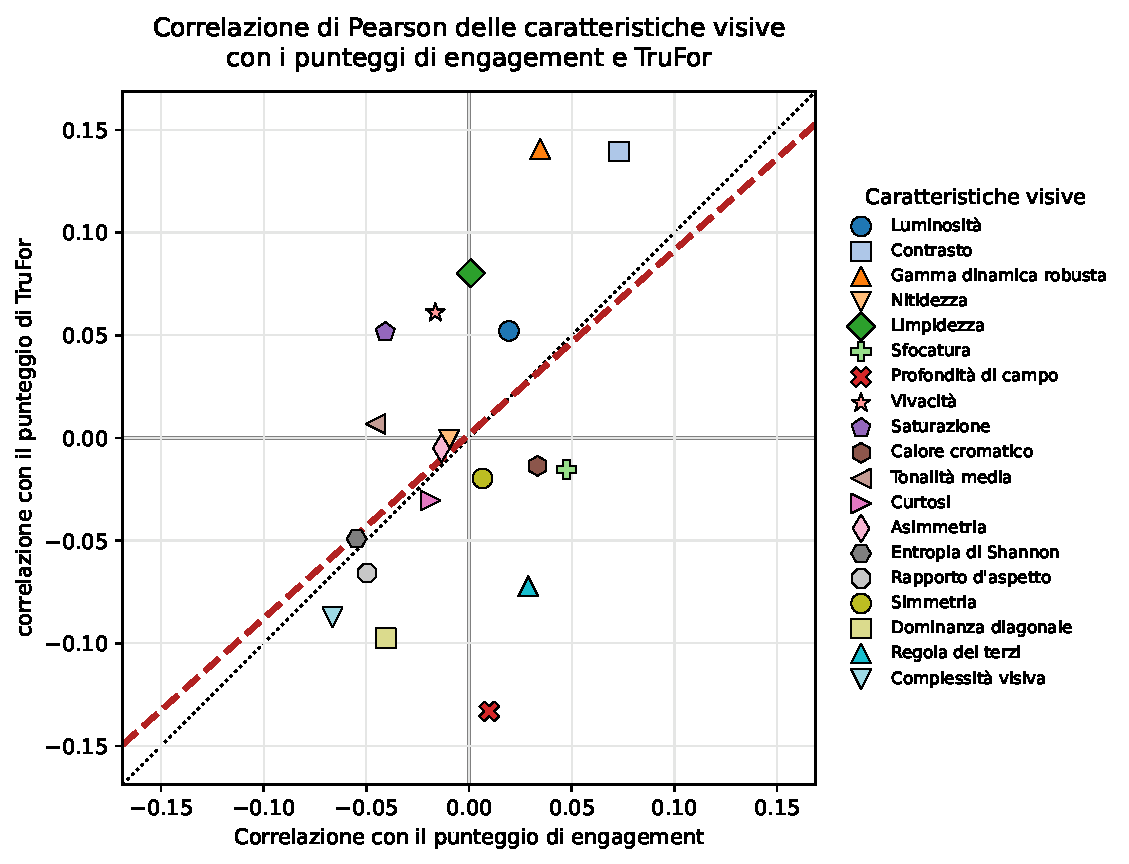
\includegraphics[width=0.8\linewidth]{caratteristiche_visive_pearson.pdf}
    \caption{Correlazioni di Pearson sulle 1.211 osservazioni. Ogni punto rappresenta una caratteristica. La retta nera puntinata indica $b=a$; quella rossa tratteggiata riassume i 19 punti. Fonte: \texttt{images\_features\_pearson.txt}.}
    \label{fig:risultati-feature-pearson}
    \par\medskip
    \captionsetup{type=figure}
    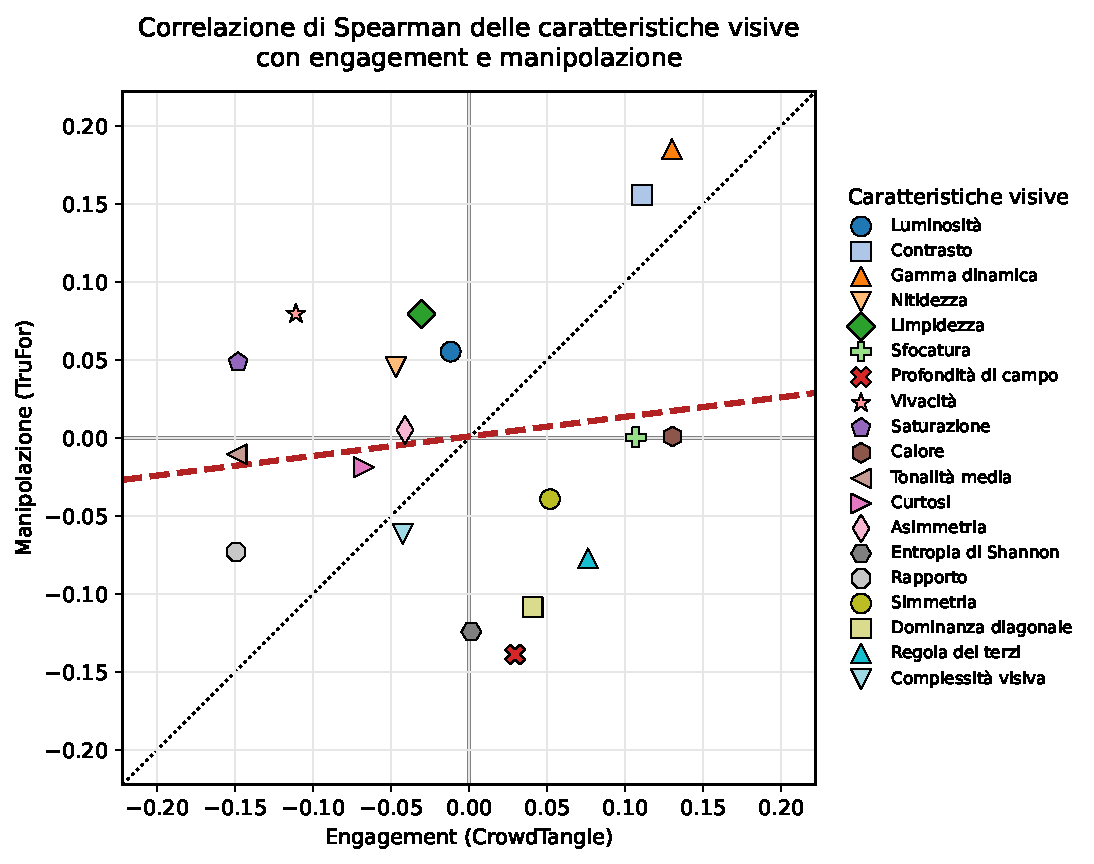
\includegraphics[width=0.8\linewidth]{caratteristiche_visive_spearman.pdf}
    \caption{Correlazioni di Spearman sulle 1.211 osservazioni. Ogni punto rappresenta una caratteristica. La retta nera puntinata indica $b=a$; quella rossa tratteggiata riassume i 19 punti. Fonte: \texttt{images\_features\_spearman.txt}.}
    \label{fig:risultati-feature-spearman}
\end{minipage}
\par\bigskip

Le caratteristiche possono essere correlate tra loro e le due coordinate derivano dallo stesso campione: la retta riassume il confronto tra descrittori e non costituisce un modello di previsione dell'engagement delle immagini. Escludo dal grafico le caratteristiche con correlazioni non definite, come avviene per una colonna costante.

Per Pearson uso \path{images_features_pearson.txt}, per Spearman uso \path{images_features_spearman.txt}. Ogni report ordina le caratteristiche per $|b_j|$ decrescente. Lo script produce coefficienti descrittivi senza valori di $p$ o intervalli di confidenza.

\subsection{Risultati delle correlazioni e lettura congiunta}
\label{subsec:associazione-visive-correlazioni}

Dispongo di tutte le variabili per le 1.211 osservazioni. La Tabella~\ref{tab:risultati-feature-correlazioni} mostra associazioni contenute con entrambi i metodi. Per l'engagement, Spearman evidenzia diverse associazioni più marcate rispetto a Pearson. Le correlazioni con TruFor mantengono più spesso segno e valori simili.

\begin{table}[htbp]
    \centering
    \small
    \caption{Correlazioni di Pearson e Spearman sulle stesse 1.211 osservazioni. Fonti: \texttt{images\_features\_pearson.txt} e \texttt{images\_features\_spearman.txt}.}
    \label{tab:risultati-feature-correlazioni}
    \begin{tabular}{@{}lrrrr@{}}
        \toprule
        & \multicolumn{2}{c}{Pearson ($r$)} & \multicolumn{2}{c}{Spearman ($\rho_s$)} \\
        \cmidrule(lr){2-3}\cmidrule(l){4-5}
        Caratteristica & Engagement & TruFor & Engagement & TruFor \\
        \midrule
        Luminosità & $+0{,}0194$ & $+0{,}0521$ & $-0{,}0118$ & $+0{,}0553$ \\
        Contrasto & $+0{,}0729$ & $+0{,}1394$ & $+0{,}1108$ & $+0{,}1559$ \\
        Gamma dinamica robusta & $+0{,}0347$ & $+0{,}1406$ & $+0{,}1300$ & $+0{,}1851$ \\
        Nitidezza & $-0{,}0097$ & $-0{,}0009$ & $-0{,}0468$ & $+0{,}0453$ \\
        Limpidezza & $+0{,}0008$ & $+0{,}0802$ & $-0{,}0305$ & $+0{,}0794$ \\
        Sfocatura & $+0{,}0474$ & $-0{,}0154$ & $+0{,}1069$ & $+0{,}0004$ \\
        Profondità di campo & $+0{,}0098$ & $-0{,}1331$ & $+0{,}0295$ & $-0{,}1388$ \\
        Vivacità & $-0{,}0164$ & $+0{,}0610$ & $-0{,}1110$ & $+0{,}0796$ \\
        Saturazione & $-0{,}0408$ & $+0{,}0516$ & $-0{,}1481$ & $+0{,}0486$ \\
        Calore & $+0{,}0334$ & $-0{,}0136$ & $+0{,}1304$ & $+0{,}0009$ \\
        Tonalità media & $-0{,}0455$ & $+0{,}0069$ & $-0{,}1490$ & $-0{,}0104$ \\
        Curtosi & $-0{,}0187$ & $-0{,}0304$ & $-0{,}0675$ & $-0{,}0188$ \\
        Asimmetria & $-0{,}0134$ & $-0{,}0050$ & $-0{,}0410$ & $+0{,}0051$ \\
        Entropia di Shannon & $-0{,}0547$ & $-0{,}0492$ & $+0{,}0014$ & $-0{,}1242$ \\
        Rapporto d'aspetto & $-0{,}0496$ & $-0{,}0658$ & $-0{,}1493$ & $-0{,}0730$ \\
        Simmetria & $+0{,}0065$ & $-0{,}0197$ & $+0{,}0519$ & $-0{,}0392$ \\
        Dominanza diagonale & $-0{,}0406$ & $-0{,}0976$ & $+0{,}0407$ & $-0{,}1084$ \\
        Regola dei terzi & $+0{,}0288$ & $-0{,}0722$ & $+0{,}0763$ & $-0{,}0772$ \\
        Complessità visiva & $-0{,}0665$ & $-0{,}0874$ & $-0{,}0425$ & $-0{,}0617$ \\
        \bottomrule
    \end{tabular}
\end{table}

Le Figure~\ref{fig:risultati-feature-pearson} e~\ref{fig:risultati-feature-spearman} rappresentano le stesse caratteristiche: la coordinata orizzontale indica la correlazione con l'engagement, quella verticale la correlazione con TruFor. Mantengo simboli e colori, adattando i limiti degli assi a ciascun metodo. La retta rossa riassume le posizioni dei 19 descrittori: presenta pendenza positiva con Pearson ed è più vicina all'orizzontale con Spearman.

Le associazioni con l'engagement restano inferiori a $0{,}15$ in valore assoluto. Il contrasto è correlato positivamente con entrambi gli indicatori; la saturazione è correlata negativamente con l'engagement e positivamente con TruFor. Per rapporto d'aspetto, tonalità media e saturazione, Spearman rileva associazioni più marcate con l'engagement rispetto a Pearson. Si tratta di confronti descrittivi, una caratteristica alla volta.

\subsection{Il blocco visivo aggiunto a TruFor}
\label{subsec:associazione-visive-glm}

Stimo un GLM non penalizzato con TruFor e le 19 caratteristiche standardizzate: sottraggo la media e divido per la deviazione standard calcolate sul campione. Ogni coefficiente visivo esprime così la variazione dei log-odds per un incremento di una deviazione standard, a parità degli altri predittori. La Tabella~\ref{tab:associazione-visive-coefficienti} riporta i coefficienti, gli intervalli al $95\%$ e i p-value non corretti dei test di Wald. Uso il test di Wald per verificare, per ciascun coefficiente, l’ipotesi nulla che sia uguale a zero~\cite{60455556-c6b2-37bb-9077-b6ce7e1443d8}.

Rispetto al solo TruFor, lo pseudo-$R^2_{\mathrm{McF}}$ passa da $0{,}0009$ a $0{,}0624$ e $Q_{\mathrm{CV}}$ da $-0{,}0060$ a $0{,}0278$. Il blocco visivo migliora quindi entrambi gli indici nel protocollo adottato. Confronto questo incremento con quello del testo nella Sezione~\ref{sec:associazione-confronto-blocchi}.

Applico Benjamini--Hochberg ai 19 p-value visivi, escludendo intercetta e TruFor dalla famiglia di verifiche~\cite{10.1111/j.2517-6161.1995.tb02031.x}. Considero significativo un coefficiente quando il valore corretto $p_{\mathrm{BH}}$, indicato con \texttt{q} nel report, è inferiore a $0{,}05$. Solo \texttt{aspect\_ratio} risulta significativo dopo la correzione: $\beta=-0{,}2177$ per deviazione standard e $p_{\mathrm{BH}}=0{,}0219<0{,}05$. La correzione riguarda il modello TruFor e visive, non il modello completo.

Il rapporto larghezza/altezza presenta un'associazione negativa condizionata agli altri predittori inclusi. Account, piattaforma e periodo rimangono fuori dal modello: non ricavo quindi una prescrizione sul formato che aumenterebbe l'engagement. I coefficienti delle altre caratteristiche, incluso il calore cromatico, non risultano significativi dopo la correzione; questo esito non prova l'assenza di una loro associazione nella popolazione.

\begin{table}[htbp]
    \centering\small
    \caption{Coefficienti delle 19 caratteristiche nel GLM TruFor e visive. Gli intervalli sono al $95\%$ e i p-value sono non corretti. Dopo Benjamini--Hochberg~\cite{10.1111/j.2517-6161.1995.tb02031.x} soltanto il rapporto d'aspetto risulta significativo, con $p_{\mathrm{BH}}=0{,}0219<0{,}05$. Fonte: \texttt{classification\_visual\_text.txt}.}
    \label{tab:associazione-visive-coefficienti}
    \begin{tabular}{@{}lrrr@{}}
        \toprule
        Caratteristica & $\beta$ per dev.\ std. & Intervallo & $p$ \\
        \midrule
        Rapporto d'aspetto & $-0{,}2177$ & $[-0{,}349;\,-0{,}086]$ & $0{,}001$ \\
        Luminosità & $-0{,}2857$ & $[-0{,}606;\,0{,}035]$ & $0{,}081$ \\
        Contrasto & $0{,}2246$ & $[-0{,}024;\,0{,}474]$ & $0{,}077$ \\
        Gamma dinamica robusta & $-0{,}0217$ & $[-0{,}215;\,0{,}171]$ & $0{,}825$ \\
        Nitidezza & $0{,}0034$ & $[-0{,}224;\,0{,}231]$ & $0{,}977$ \\
        Limpidezza & $-0{,}0584$ & $[-0{,}372;\,0{,}256]$ & $0{,}716$ \\
        Sfocatura & $0{,}1471$ & $[-0{,}018;\,0{,}313]$ & $0{,}082$ \\
        Profondità di campo & $-0{,}0425$ & $[-0{,}183;\,0{,}098]$ & $0{,}553$ \\
        Vivacità & $-0{,}0119$ & $[-0{,}258;\,0{,}234]$ & $0{,}925$ \\
        Saturazione & $-0{,}2719$ & $[-0{,}527;\,-0{,}017]$ & $0{,}037$ \\
        Calore & $0{,}2072$ & $[0{,}058;\,0{,}357]$ & $0{,}007$ \\
        Tonalità media & $-0{,}0551$ & $[-0{,}217;\,0{,}107]$ & $0{,}505$ \\
        Curtosi & $-0{,}0332$ & $[-0{,}272;\,0{,}206]$ & $0{,}785$ \\
        Asimmetria & $-0{,}1498$ & $[-0{,}467;\,0{,}167]$ & $0{,}355$ \\
        Entropia di Shannon & $-0{,}0419$ & $[-0{,}273;\,0{,}189]$ & $0{,}723$ \\
        Simmetria & $0{,}1798$ & $[0{,}033;\,0{,}326]$ & $0{,}016$ \\
        Dominanza diagonale & $0{,}0103$ & $[-0{,}166;\,0{,}186]$ & $0{,}909$ \\
        Regola dei terzi & $0{,}1184$ & $[-0{,}026;\,0{,}263]$ & $0{,}109$ \\
        Complessità visiva & $0{,}1344$ & $[-0{,}066;\,0{,}335]$ & $0{,}189$ \\
        \bottomrule
    \end{tabular}
\end{table}

\newpage
\section{Contributo del testo delle regioni sospette}
\label{sec:associazione-testo}

Valuto due rappresentazioni dello stesso testo: i pesi delle parole e le componenti PCA. In entrambi i casi includo il punteggio TruFor. Distinguo le prestazioni della logistica regolarizzata dalla stima dei GLM, perché rispondono a finalità diverse.

\subsection{Preparazione e rappresentazioni testuali}
\label{subsec:associazione-testo-preparazione}

Rimuovo le stop word italiane e inglesi, normalizzate come le descrizioni, e \texttt{nomask}. Estraggo unigrammi di almeno due caratteri. Conservo i termini presenti in almeno cinque descrizioni e in non più del $40\%$ del campione; fra quelli ammessi mantengo al massimo i cento più frequenti.

Indico con $n_{ij}$ le occorrenze della parola $j$ nella descrizione $i$ e con $d_j$ il numero di descrizioni che la contengono. Uso la variante TF-IDF con regolarizzazione delle frequenze documentali~\cite{scikit-learn}:
\begin{equation}
    a_{ij}=n_{ij}\left[1+\log\left(\frac{1+n}{1+d_j}\right)\right],
    \qquad x_{ij}=\frac{a_{ij}}{\sqrt{\sum_k a_{ik}^2}}.
    \label{eq:classificazione-tfidf}
\end{equation}
Normalizzo ogni riga alla norma euclidea unitaria. Se nessun termine appartiene al vocabolario, mantengo un vettore nullo. Questo accade anche per \texttt{nomask}: la codifica unisce quindi assenza di descrizione e assenza di parole conservate dai filtri.

Per la seconda rappresentazione centro le colonne TF-IDF, senza standardizzarle, e applico la PCA~\cite{jolliffe2016principal}. Fisso la varianza da conservare al $90\%$ e ottengo 61 componenti. Una riga TF-IDF nulla può avere coordinate PCA diverse da zero per effetto della centratura. TruFor rimane separato e non entra nella PCA.

Per i GLM regolarizzati indico con $\alpha$ l'intensità della penalizzazione. La \emph{penalità L1}, detta \emph{lasso}, usa la somma dei valori assoluti dei coefficienti; \emph{elastic net} combina L1 e L2. La quota L1 regola questa combinazione: 0 corrisponde a ridge, 1 a lasso e i valori intermedi a elastic net. Riassumo la configurazione nella Tabella~\ref{tab:classificazione-parametri}.

\begin{table}[htbp]
    \centering
    \small
    \caption{Configurazione della classificazione. I parametri condivisi provengono da \texttt{scripts/config.py}; la logistica usa le impostazioni predefinite di scikit-learn~\cite{scikit-learn} salvo il limite di iterazioni.}
    \label{tab:classificazione-parametri}
    \begin{tabular}{@{}lr@{}}
        \toprule
        Parametro & Valore \\
        \midrule
        Intervallo escluso per l'engagement & $[-0{,}5;\,0{,}5]$ \\
        Vocabolario massimo & 100 unigrammi \\
        Frequenza documentale minima / massima & 5 / $40\%$ \\
        Varianza da conservare con PCA & $90\%$ \\
        Logistica: penalità / parametro $C$ & L2 / 1 \\
        Logistica: massimo di iterazioni & 1.000 \\
        GLM: penalità di ripiego $\alpha$ / quota L1 & $0{,}0007$ / 0 \\
        Partizioni di validazione & 5 \\
        Permutazioni per predittore & 30 \\
        Casi spiegati con LIME & 5 \\
        \bottomrule
    \end{tabular}
\end{table}

\subsection{Prestazioni della regressione logistica}
\label{subsec:risultati-classificazione-logistica}

Con \path{classification_logistic_regression.py} addestro la logistica L2, con $C=1$ e massimo 1.000 iterazioni. Uso \texttt{cross\_val\_predict} con le cinque partizioni stratificate della Sottosezione~\ref{subsec:metodi-classificazione-validazione}. Per gli odds ratio riaddestro invece il modello sull'intero campione.

La Tabella~\ref{tab:risultati-classificazione-logistica} confronta cento parole TF-IDF e 61 componenti PCA, sempre con TruFor. Ottengo un'accuratezza del $59{,}4\%$, circa 8,2 punti percentuali sopra la baseline del $51{,}2\%$. Il TF-IDF presenta AUC e $Q_{\mathrm{CV}}$ leggermente maggiori. La riduzione dei predittori conserva quindi una prestazione vicina a quella della rappresentazione lessicale.

\begin{table}[htbp]
    \centering
    \small
    \caption{Regressione logistica L2 sulle due rappresentazioni testuali, entrambe con TruFor. Metriche sulle previsioni riunite delle cinque partizioni; baseline di maggioranza: $51{,}2\%$. Fonte: \texttt{classification\_logistic\_regression.txt}.}
    \label{tab:risultati-classificazione-logistica}
    \begin{tabular}{@{}lrrrr@{}}
        \toprule
        Testo & Predittori & Accuratezza & AUC & $Q_{\mathrm{CV}}$ \\
        \midrule
        TF-IDF & 101 & $59{,}4\%$ & $0{,}644$ & $0{,}0613$ \\
        TF-IDF con PCA & 62 & $59{,}4\%$ & $0{,}638$ & $0{,}0582$ \\
        \bottomrule
    \end{tabular}
\end{table}

Entrambe le configurazioni classificano correttamente 710 casi (Tabella~\ref{tab:associazione-confusioni}). Restano 485 errori: le rappresentazioni mostrano una capacità predittiva modesta. I report non forniscono intervalli d'incertezza per le differenze fra le prestazioni.

\begin{table}[htbp]
    \centering\small
    \caption{Conteggi delle matrici di confusione in validazione, con classe positiva 1 e soglia $0{,}5$. TP (True Positives) e TN (True Negatives) indicano rispettivamente i veri positivi e i veri negativi; FP (False Positives) e FN (False Negatives) indicano i falsi positivi e i falsi negativi. Fonte: \texttt{classification\_logistic\_regression.txt}.}
    \label{tab:associazione-confusioni}
    \begin{tabular}{@{}lrrrrr@{}}
        \toprule
        Testo, con TruFor & TP & TN & FP & FN & \shortstack{Previsioni\\corrette} \\
        \midrule
        TF-IDF & 293 & 417 & 195 & 290 & 710 \\
        TF-IDF con PCA & 297 & 413 & 199 & 286 & 710 \\
        \bottomrule
    \end{tabular}
\end{table}

\subsection{Stima dei GLM sulle rappresentazioni testuali}
\label{subsec:associazione-testo-glm}

Con \path{classification_glm.py} stimo i GLM per massima verosimiglianza tramite \emph{IRLS (Iteratively Reweighted Least Squares)}, cioè minimi quadrati iterativamente ripesati. Includo l'intercetta e controllo convergenza e finitezza della log-verosimiglianza. Se il controllo fallisce, uso ridge con $\alpha=0{,}0007$, senza errori standard o p-value. La regolarizzazione stabilizza la stima in presenza di problemi come la separazione; il solo fallimento numerico non ne costituisce una diagnosi completa~\cite{10.1093/biomet/71.1.1}.

Sul TF-IDF il GLM non penalizzato non supera il controllo di convergenza e ricorro al fit ridge (Tabella~\ref{tab:associazione-glm-testo}). Sulle componenti PCA il GLM converge. In quest'ultimo modello, il coefficiente di TruFor è $0{,}4998$, con intervallo al $95\%$ $[-0{,}033;\,1{,}033]$ e $p=0{,}066$. I coefficienti delle componenti combinano più parole: i loro test non identificano singoli termini associati all'engagement.

\begin{table}[htbp]
    \centering\small
    \caption{GLM sulle due rappresentazioni testuali, con TruFor. L'indice riguarda i dati di stima. Fonte: \texttt{classification\_glm.txt}.}
    \label{tab:associazione-glm-testo}
    \begin{tabular}{@{}lrrl@{}}
        \toprule
        Testo & Predittori & $R^2_{\mathrm{McF}}$ & Stima utilizzata \\
        \midrule
        TF-IDF & 101 & $0{,}1383$ & Ridge, senza p-value \\
        TF-IDF con PCA & 62 & $0{,}1369$ & Non penalizzata \\
        \bottomrule
    \end{tabular}
\end{table}

\newpage
\subsection{Interpretazione del contributo testuale}
\label{subsec:associazione-testo-interpretazione}

Il GLM con testo PCA raggiunge $Q_{\mathrm{CV}}=0{,}0234$, rispetto a $-0{,}0060$ del solo TruFor, nelle stesse partizioni. Il risultato sostiene l'utilità di studiare il contenuto selezionato, entro i limiti del protocollo. Non dimostra che descrivere le regioni sospette sia meglio che descrivere l'immagine intera: manca un classificatore basato su descrizioni dell'immagine intera ottenute con gli stessi strumenti. Il contributo osservato appartiene alla rappresentazione prodotta dalla pipeline nel suo insieme.

\section{Ricerca esplorativa degli iperparametri}
\label{sec:associazione-grid-search}

Applico la grid search introdotta nella Sottosezione~\ref{subsec:metodi-classificazione-validazione} tramite la modalità \texttt{--grid-search} di \path{classification_glm.py} per esplorare i filtri documentali e la penalità del GLM sul TF-IDF, sempre insieme a TruFor. Il parametro $\alpha$ controlla l'intensità della penalità; la quota L1 ne distingue la componente lasso da quella ridge. La ricerca non usa la PCA e non seleziona il parametro $C$ della logistica L2. Considero le combinazioni della Tabella~\ref{tab:associazione-grid-parametri}, mantenendo il limite di cento parole e lo stesso campione di 1.195 osservazioni.

\begin{table}[htbp]
    \centering\small
    \caption{Griglia esplorata, da \texttt{classification\_glm\_grid\_search.txt}. La quota L1 distingue ridge (0), elastic net ($0{,}5$) e lasso (1).}
    \label{tab:associazione-grid-parametri}
    \begin{tabular}{@{}lp{0.62\linewidth}@{}}
        \toprule
        Parametro & Valori \\
        \midrule
        \texttt{min\_df} & 2, 5, 10 descrizioni \\
        \texttt{max\_df} & $0{,}4$; $0{,}5$; $0{,}6$; $0{,}7$; $0{,}8$ \\
        Penalità $\alpha$ & 0; $0{,}0001$; $0{,}0005$; $0{,}0007$; $0{,}001$; $0{,}005$; $0{,}01$ \\
        Quota L1 & 0; $0{,}5$; 1, solo per $\alpha>0$ \\
        Totale & $3\times5\times(1+6\times3)=285$ configurazioni \\
        \bottomrule
    \end{tabular}
\end{table}

Per ogni coppia di filtri ricostruisco il TF-IDF sull'intero campione. Valuto poi le penalità con cinque partizioni non stratificate, mescolate con seme 42, e ordino le configurazioni per $Q_{\mathrm{CV}}$. Per $\alpha=0$ eseguo una sola valutazione, perché la quota L1 non modifica il modello. Controllo inoltre se il GLM non penalizzato converge su tutto il campione per ciascuna coppia di filtri.

Ottengo un punteggio per le 270 configurazioni penalizzate; le 15 non penalizzate non superano la valutazione nelle partizioni. Inoltre, nessuna delle 15 coppie di filtri produce un GLM non penalizzato convergente sull'intero campione. Il report non individua quindi una configurazione che conservi i p-value del fit non penalizzato.

Il massimo è $Q_{\mathrm{CV}}=0{,}0647$, con \texttt{min\_df}=5, \texttt{max\_df}=$0{,}4$ e ridge con $\alpha=0{,}0007$ (Tabella~\ref{tab:associazione-grid-risultati}). Questi valori coincidono con la configurazione adottata. La ricerca documenta la scelta dei parametri, ma il massimo è selezionato sullo stesso campione e sulle stesse partizioni usate per confrontare le configurazioni. Non lo considero una stima indipendente della prestazione: servirebbe una valutazione esterna alla selezione degli iperparametri.

\begin{table}[htbp]
    \centering\small
    \caption{Migliore configurazione riportata per ciascuna famiglia di penalità. Tutte conservano cento parole. Le altre quattro soglie \texttt{max\_df} danno lo stesso punteggio arrotondato per ciascuna riga. Fonte: \texttt{classification\_glm\_grid\_search.txt}.}
    \label{tab:associazione-grid-risultati}
    \begin{tabular}{@{}lrrrrr@{}}
        \toprule
        Penalità & \texttt{min\_df} & \texttt{max\_df} & $\alpha$ & Quota L1 & $Q_{\mathrm{CV}}$ \\
        \midrule
        Ridge & 5 & $0{,}4$ & $0{,}0007$ & 0 & $0{,}0647$ \\
        Elastic net & 5 & $0{,}4$ & $0{,}0007$ & $0{,}5$ & $0{,}0596$ \\
        Lasso & 2 & $0{,}4$ & $0{,}001$ & 1 & $0{,}0556$ \\
        \bottomrule
    \end{tabular}
\end{table}

\section{Confronto dei blocchi informativi}
\label{sec:associazione-confronto-blocchi}

Con \path{classification_visual_text.py} confronto quattro GLM non penalizzati sulle stesse 1.195 osservazioni e con le stesse partizioni: TruFor; TruFor e testo PCA; TruFor e caratteristiche visive; tutti i predittori insieme. I modelli includono l'intercetta, esclusa dal conteggio dei predittori. Il testo descrive le regioni sospette, mentre le 19 caratteristiche standardizzate descrivono l'immagine intera.

La Tabella~\ref{tab:risultati-confronto-blocchi} e la Figura~\ref{fig:classificazione-confronto-modelli} mostrano un miglioramento rispetto al solo TruFor quando aggiungo separatamente testo o caratteristiche visive. Il modello con le caratteristiche visive ottiene il maggiore $Q_{\mathrm{CV}}$, ma la differenza rispetto al testo è contenuta e non dispone di un intervallo d'incertezza.

\begin{table}[htbp]
    \centering
    \small
    \caption{Confronto dei blocchi sul medesimo campione di 1.195 osservazioni. Distinguo lo pseudo-$R^2$ in-sample dall'indice $Q_{\mathrm{CV}}$ calcolato con cinque partizioni comuni ai quattro GLM. Fonte: \texttt{classification\_visual\_text.txt}.}
    \label{tab:risultati-confronto-blocchi}
    \begin{tabular}{@{}lrrr@{}}
        \toprule
        Predittori & Numero & $R^2_{\mathrm{McF}}$ & $Q_{\mathrm{CV}}$ \\
        \midrule
        TruFor & 1 & $0{,}0009$ & $-0{,}0060$ \\
        TruFor e testo & 62 & $0{,}1369$ & $0{,}0234$ \\
        TruFor e visive & 20 & $0{,}0624$ & $0{,}0278$ \\
        TruFor, testo e visive & 81 & $0{,}1605$ & $0{,}0128$ \\
        \bottomrule
    \end{tabular}
\end{table}

\begin{figure}[htbp]
    \centering
    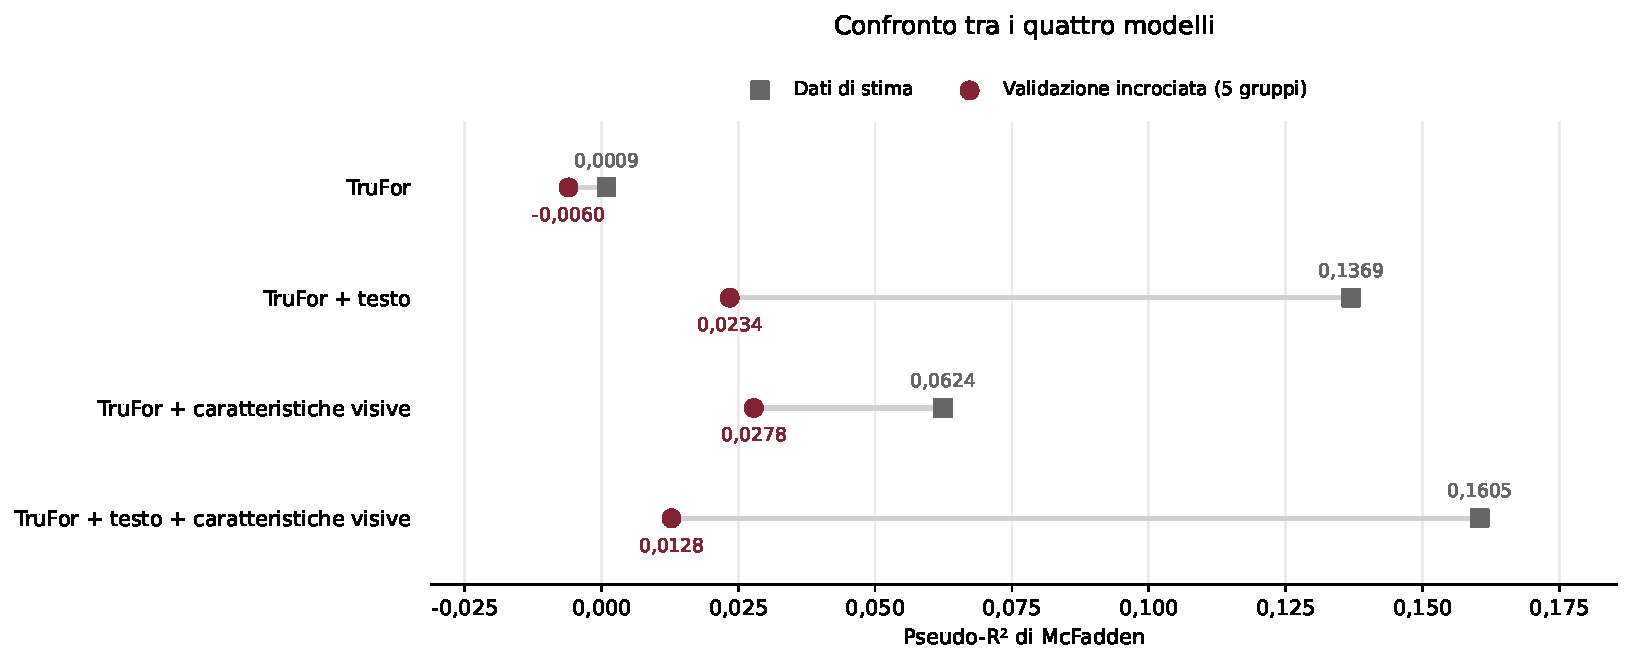
\includegraphics[width=\linewidth]{classificazione_confronto_modelli.pdf}
    \caption{Adattamento e validazione dei quattro GLM. I quadrati indicano $R^2_{\mathrm{McF}}$ sui dati di stima; i cerchi indicano $Q_{\mathrm{CV}}$ in validazione incrociata. Valori più alti indicano un risultato migliore; zero corrisponde al riferimento basato sulla frequenza delle classi e valori negativi indicano un risultato peggiore del riferimento. La validazione riguarda la stima dei coefficienti del modello: TF-IDF, PCA e standardizzazione sono stimati sull'intero campione. Fonte: \texttt{classification\_visual\_text.txt}.}
    \label{fig:classificazione-confronto-modelli}
\end{figure}

\newpage
Il modello completo raggiunge il maggiore adattamento in-sample, $0{,}1605$, ma $Q_{\mathrm{CV}}$ scende a $0{,}0128$. Aggiungere le caratteristiche visive al testo migliora quindi il fit sui dati di stima senza migliorare la prestazione nel protocollo adottato. Per rispondere anche alla domanda sul contributo aggiuntivo delle descrizioni, confronto il modello completo con quello che comprende già TruFor e le caratteristiche visive: aggiungendo il testo, $Q_{\mathrm{CV}}$ passa da $0{,}0278$ a $0{,}0128$. Nel confronto osservato il testo non migliora quindi questo riferimento più informativo, pur migliorando quello basato sul solo TruFor. Un maggiore numero di coefficienti può rendere la stima più sensibile al campione. Anche una sovrapposizione fra informazioni visive e testuali è possibile, ma il risultato non dimostra che i due blocchi siano ridondanti.

Confronto inoltre le coppie di \emph{modelli annidati}: in questi confronti ottengo il modello ridotto ponendo a zero i coefficienti dei predittori aggiunti nel modello esteso. Uso la \emph{devianza} $D=2(\ell_{\mathrm{saturo}}-\ell_{\mathrm{modello}})$, che confronta la log-verosimiglianza del modello con quella del \emph{modello saturo}, capace di riprodurre esattamente ogni osservazione. La statistica del \emph{test del rapporto di verosimiglianza} è $\Lambda=D_{\mathrm{ridotto}}-D_{\mathrm{esteso}}$. Sotto l'ipotesi nulla e le condizioni di regolarità uso il riferimento asintotico $\chi^2$, con gradi di libertà pari al numero dei parametri aggiunti. Confronto ciascun modello intermedio con TruFor e il completo con TruFor e testo. I due modelli intermedi non sono annidati fra loro.

I test della Tabella~\ref{tab:associazione-rapporti-verosimiglianza} riguardano i coefficienti aggiunti sotto le ipotesi del GLM. Il risultato del modello completo rende concreta la distinzione: un test significativo accompagna un peggioramento in validazione. La significatività statistica non garantisce un vantaggio predittivo su nuovi dati.

\begin{table}[htbp]
    \centering\small
    \caption{Test del rapporto di verosimiglianza tra GLM annidati. I due valori di $p$ arrotondati a zero nel report sono indicati con $p<0{,}0001$. Fonte: \texttt{classification\_visual\_text.txt}.}
    \label{tab:associazione-rapporti-verosimiglianza}
    \begin{tabular}{@{}lrrr@{}}
        \toprule
        Estensione del modello & $\Lambda$ & Gradi di libertà & $p$ \\
        \midrule
        TruFor $\rightarrow$ TruFor e testo & $225{,}2$ & 61 & $<0{,}0001$ \\
        TruFor $\rightarrow$ TruFor e visive & $101{,}8$ & 19 & $<0{,}0001$ \\
        TruFor e testo $\rightarrow$ completo & $38{,}9$ & 19 & $0{,}0045$ \\
        \bottomrule
    \end{tabular}
\end{table}

Rispetto alla domanda di ricerca, osservo un contributo predittivo modesto delle rappresentazioni arricchite. Il testo e le caratteristiche visive aggiunti separatamente migliorano il riferimento TruFor. Il confronto con il modello che include già le caratteristiche visive non mostra invece un vantaggio predittivo aggiuntivo delle descrizioni. Questa conclusione riguarda il campione e il protocollo adottati, con preparazione dei predittori prima della suddivisione; non dimostra l'assenza di informazione utile nel testo in altri campioni o con altre rappresentazioni.

\section{Interpretazione delle previsioni sulle parole}
\label{sec:associazione-spiegazioni}

Con \path{classification_lime_shap.py} riaddestro la logistica su TruFor e sulle cento colonne TF-IDF dell'intero campione. Ispeziono il modello attraverso il report \path{classification_explanations.txt}. Le misure riguardano le osservazioni usate per stimarlo e non costituiscono una nuova valutazione predittiva.

\subsection{Protocollo delle spiegazioni}
\label{subsec:metodi-classificazione-spiegazioni}

Calcolo l'importanza per permutazione~\cite{JMLR:v20:18-760} come calo dell'AUC sul campione di stima. Ripeto il rimescolamento trenta volte per predittore, con seme 42. Riporto media e deviazione standard: quest'ultima descrive le permutazioni a modello fisso, non l'incertezza dovuta a nuovi campioni. Il criterio del report ``media maggiore di due deviazioni standard'' è descrittivo e non sostituisce un p-value.

Per SHAP~\cite{NIPS2017_8a20a862} uso il \emph{mascheramento indipendente} delle variabili tabulari: i valori delle variabili temporaneamente escluse vengono sostituiti con quelli del campione di riferimento, senza condizionarli ai valori delle variabili mantenute. L'operazione riguarda le colonne TruFor e TF-IDF, non i pixel dell'immagine; uso tutte le osservazioni come riferimento. In questa configurazione il contributo della variabile $j$ al predittore lineare è $\phi_{ij}=\beta_j(u_{ij}-\bar u_j)$, espresso nei log-odds. Ordino le variabili tramite la media $n^{-1}\sum_i|\phi_{ij}|$ e ricavo la direzione dal segno del coefficiente logistico. La media dei contributi con segno sullo stesso riferimento è invece nulla.

Per LIME uso la variante tabulare senza discretizzare le variabili continue, con seme 42. Con le impostazioni predefinite, genero le perturbazioni campionando indipendentemente i valori TF-IDF e TruFor da distribuzioni normali con media e deviazione standard stimate sull'intero campione. Adatto una regressione ridge alle probabilità della classe 1 prodotte dal classificatore per questi dati. Assegno alle perturbazioni pesi che diminuiscono esponenzialmente con il quadrato della distanza euclidea dall'osservazione da spiegare, calcolata sulle variabili standardizzate: i punti più vicini incidono quindi maggiormente sul surrogato locale~\cite{ribeiro2016whyitrustyou}. Seleziono cinque osservazioni a posizioni equidistanti nell'ordinamento delle probabilità previste. I coefficienti del surrogato possono riguardare anche termini assenti dalla descrizione: non rappresentano automaticamente contributi additivi alla singola previsione.

\subsection{Coefficienti, frequenza e importanza globale}
\label{subsec:risultati-spiegazioni-globali}

La Figura~\ref{fig:classificazione-parole} affianca tre quantità: il coefficiente logistico, la quota di descrizioni contenenti una parola e la media dei suoi valori SHAP assoluti. Quest'ultima determina l'area delle bolle. La frequenza è mostrata su scala logaritmica. Un coefficiente di ampiezza elevata può riguardare una parola rara: la lettura congiunta evita di confondere l'ampiezza del coefficiente con l'importanza media nel campione.

La Figura~\ref{fig:classificazione-parole-barre} riporta le otto parole con maggiore media $|\mathrm{SHAP}|$ per ciascun segno del coefficiente. I valori sono espressi nei log-odds, non in punti percentuali di probabilità.

\newpage
\begin{figure}[htbp]
    \centering
    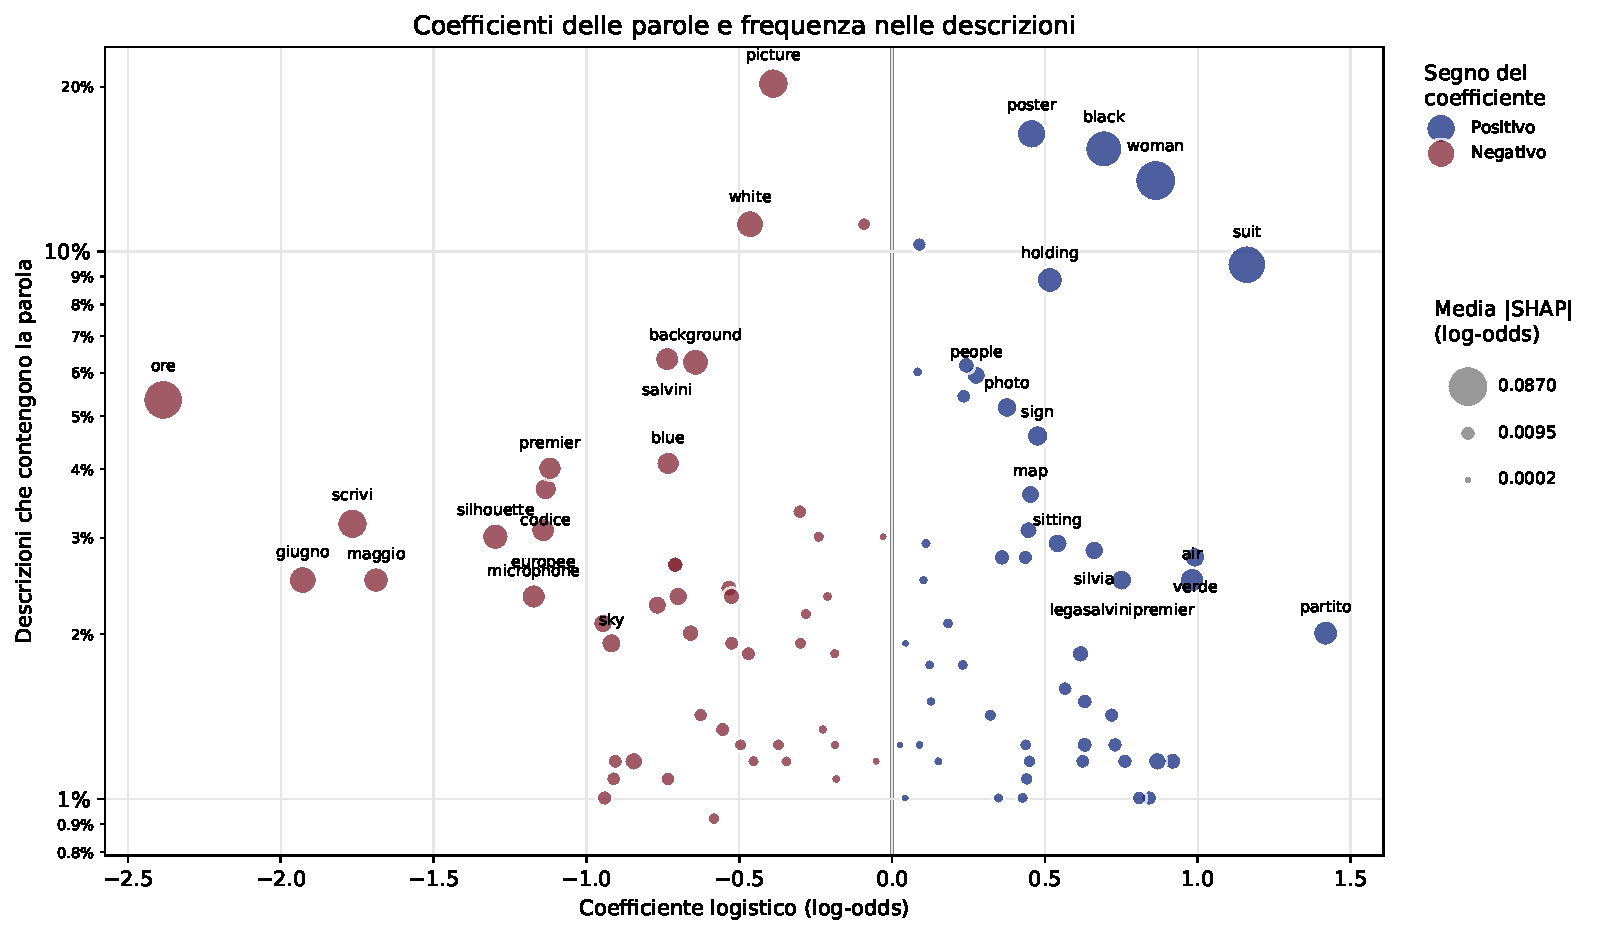
\includegraphics[width=\linewidth]{classificazione_parole.pdf}
    \caption{Coefficienti e frequenza delle parole nella logistica stimata sull'intero campione a fini interpretativi. L'area delle bolle indica la media $|\mathrm{SHAP}|$, prodotto tra $|\beta|$ e scarto assoluto medio dei valori TF-IDF: non è una misura indipendente. La distanza da zero non indica significatività; i p-value non sono disponibili perché il GLM sul TF-IDF grezzo non converge. I segni descrivono la previsione, non effetti causali.}
    \label{fig:classificazione-parole}
\end{figure}

\begin{figure}[htbp]
    \centering
    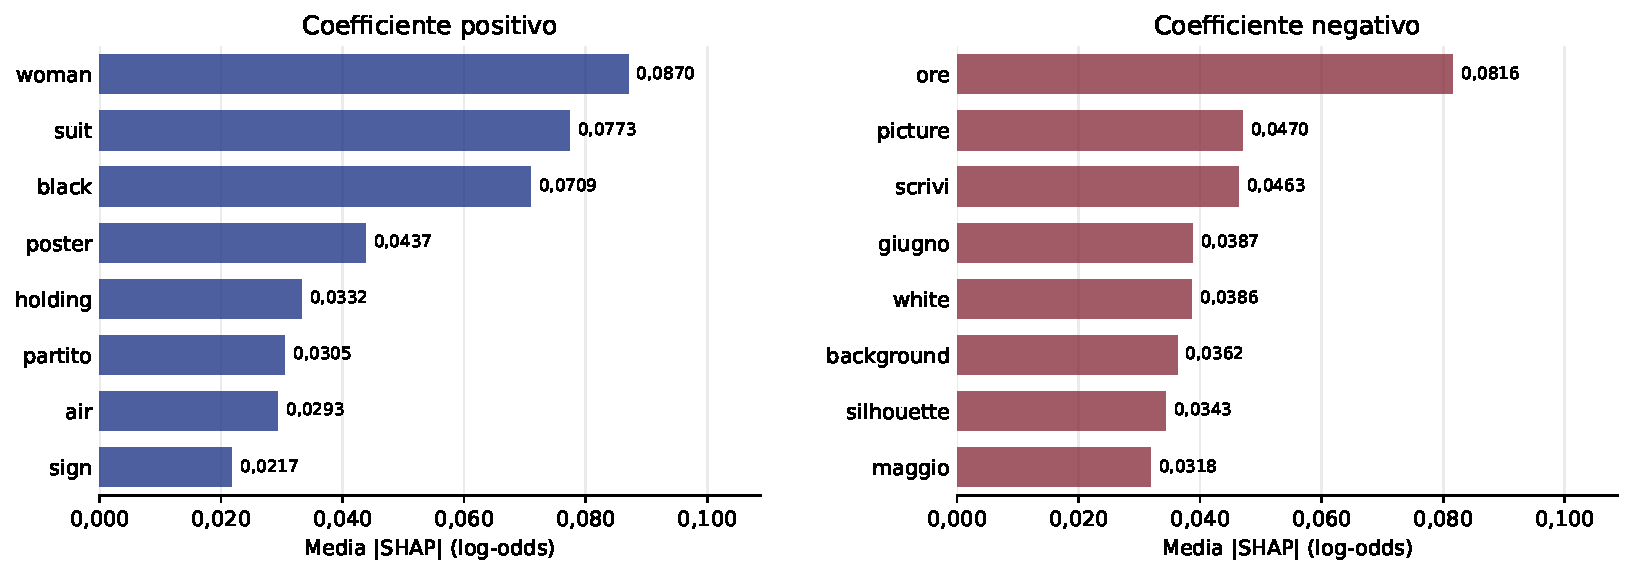
\includegraphics[width=\linewidth]{classificazione_parole_barre.pdf}
    \caption{Otto parole più importanti per media $|\mathrm{SHAP}|$~\cite{NIPS2017_8a20a862} sul campione di stima, divise per segno del coefficiente. I valori sono nei log-odds, non variazioni percentuali di probabilità, effetti causali o misure di significatività. Fonte: \texttt{classification\_explanations.txt}.}
    \label{fig:classificazione-parole-barre}
\end{figure}

Le due misure della Tabella~\ref{tab:associazione-parole-importanza} rispondono a domande diverse. SHAP scompone il predittore rispetto al riferimento; la permutazione valuta il cambiamento di una metrica quando rimescolo una colonna. La concordanza su alcuni termini non costituisce una conferma indipendente, perché entrambe usano lo stesso modello e campione.

\begin{table}[htbp]
    \centering\small
    \caption{Confronto fra SHAP~\cite{NIPS2017_8a20a862} e importanza per permutazione~\cite{JMLR:v20:18-760} per le due parole principali di ciascun segno nella Figura~\ref{fig:classificazione-parole-barre}. Dispersione su 30 permutazioni a modello fisso. Fonte: \texttt{classification\_explanations.txt}.}
    \label{tab:associazione-parole-importanza}
    \begin{tabular}{@{}lcrr@{}}
        \toprule
        Parola & Segno di $\beta$ & Media $|\mathrm{SHAP}|$ & Calo AUC: media $\pm$ dev.\ std. \\
        \midrule
        \texttt{woman} & $+$ & $0{,}0870$ & $0{,}0098\pm0{,}0042$ \\
        \texttt{suit} & $+$ & $0{,}0773$ & $0{,}0127\pm0{,}0043$ \\
        \texttt{ore} & $-$ & $0{,}0816$ & $0{,}0146\pm0{,}0059$ \\
        \texttt{picture} & $-$ & $0{,}0470$ & $0{,}0028\pm0{,}0036$ \\
        \bottomrule
    \end{tabular}
\end{table}

\newpage
Leggo le parole come indizi della rappresentazione automatica. Poiché il testo combina BLIP e OCR, termini relativi a persone, abbigliamento, date o manifesti possono riflettere il contenuto, gli autori dei post, gli errori di trascrizione o le caratteristiche del mascheramento. I coefficienti non permettono di separare queste spiegazioni.

\subsection{Due esempi locali con LIME}
\label{subsec:risultati-spiegazioni-locali}

Mostro i due casi estremi fra i cinque selezionati, identificati dai primi otto caratteri del nome del file. Il caso \texttt{c43374c2} ha $\widehat p=0{,}05$ e classe osservata 0: la descrizione menziona un uomo davanti a un televisore e contiene \texttt{ore} e \texttt{maggio}. Il caso \texttt{ca9681c6} ha $\widehat p=0{,}86$ e classe osservata 1: la stringa menziona un manifesto con un uomo e una donna e include \texttt{partito}.

Nella Tabella~\ref{tab:risultati-lime}, il peso di \texttt{ore} nel secondo caso descrive la sensibilità del surrogato alle perturbazioni, benché il termine sia assente.

\begin{table}[!htbp]
    \centering
    \small
    \caption{Coefficienti LIME~\cite{ribeiro2016whyitrustyou} dei due casi estremi sul campione di stima. ``Presente'' indica se il termine compare nella descrizione. Fonte: \texttt{classification\_explanations.txt}.}
    \label{tab:risultati-lime}
    \begin{tabular}{@{}llcr@{}}
        \toprule
        Caso & Termine & Presente & Coefficiente LIME \\
        \midrule
        \texttt{c43374c2} & \texttt{ore} & Sì & $-0{,}041$ \\
                           & \texttt{maggio} & Sì & $-0{,}018$ \\
                           & \texttt{woman} & No & $+0{,}033$ \\
        \addlinespace
        \texttt{ca9681c6} & \texttt{woman} & Sì & $+0{,}034$ \\
                           & \texttt{partito} & Sì & $+0{,}025$ \\
                           & \texttt{ore} & No & $-0{,}043$ \\
        \bottomrule
    \end{tabular}
\end{table}

% !TeX root = ../tesi.tex
% !TeX encoding = UTF-8
% !TeX spellcheck = it_IT

\chapter{Conclusioni, limitazioni e sviluppi futuri}
\label{chap:conclusioni-limitazioni-sviluppi}
% Conservo i rimandi ai due capitoli precedenti, ora riuniti.
\label{chap:conclusioni}
\label{chap:limiti}

In questo capitolo sintetizzo la risposta alla domanda di ricerca (Sezione~\ref{sec:conclusioni-risposta}) e il contributo del progetto (Sezione~\ref{sec:conclusioni-contributo}). Delimito poi le conclusioni attraverso i limiti del campione, delle rappresentazioni e della valutazione (Sezione~\ref{sec:conclusioni-limitazioni}). Infine propongo le verifiche successive (Sezione~\ref{sec:conclusioni-sviluppi}).

\section{Risposta alla domanda di ricerca}
\label{sec:conclusioni-risposta}

La domanda iniziale riguarda il contributo del contenuto delle regioni sospette e delle caratteristiche visive alla classificazione dell'engagement, rispetto al solo punteggio TruFor. Nel campione analizzato osservo un contributo predittivo modesto delle rappresentazioni arricchite. Testo e caratteristiche visive, aggiunti separatamente, migliorano il confronto con il punteggio forense; la loro combinazione non produce un ulteriore miglioramento in validazione.

Sul campione finale di 1.195 osservazioni, la logistica con TruFor e testo TF-IDF raggiunge il $59{,}4\%$ di accuratezza, contro la baseline di maggioranza del $51{,}2\%$, e AUC $0{,}644$ (Tabella~\ref{tab:risultati-classificazione-logistica}). Nel confronto tra GLM sulle stesse partizioni, $Q_{\mathrm{CV}}$ passa da $-0{,}0060$ per il solo TruFor a $0{,}0234$ con il testo e a $0{,}0278$ con le caratteristiche visive. Il modello completo raggiunge il maggiore pseudo-$R^2$ sui dati di stima, pari a $0{,}1605$, ma il suo indice in validazione scende a $0{,}0128$ (Tabella~\ref{tab:risultati-confronto-blocchi}). Il migliore adattamento al campione non si traduce quindi nella migliore prestazione sulle partizioni escluse dalla stima.

Questi risultati sostengono l'utilità di esaminare informazioni più articolate del solo punteggio TruFor, entro il protocollo adottato. Non dimostrano che testo e caratteristiche visive siano ridondanti, né che descrivere le regioni sospette sia preferibile a descrivere l'immagine intera. Studio inoltre associazioni con l'engagement osservato, senza identificare effetti causali delle modifiche alle immagini sulle interazioni degli utenti.

\section{Contributo del progetto}
\label{sec:conclusioni-contributo}

Realizzo una pipeline che collega immagini politiche, indizi forensi e misure di engagement. Integro i modelli preaddestrati di TruFor, BLIP ed EasyOCR con il filtraggio dei dati, il mascheramento, l'estrazione delle caratteristiche visive e le analisi statistiche. Il contributo consiste nell'integrazione di questi componenti e nel confronto delle rappresentazioni ottenute.

Mantengo distinti il ramo che descrive le regioni sospette e quello che misura le 19 caratteristiche dell'immagine intera. Raccolgo gli output in una tabella comune e li collego agli originali mediante l'identificatore del file. Le mappe, le immagini mascherate e i testi intermedi permettono di ispezionare il passaggio dall'immagine ai predittori; i parametri centralizzati permettono di ripetere l'elaborazione con configurazioni diverse (Sezione~\ref{subsec:pipeline-output}).

Il confronto sul medesimo campione distingue il contributo di TruFor, del testo e delle caratteristiche visive. Affianco alla valutazione predittiva l'analisi dei coefficienti e le spiegazioni delle previsioni. Ottengo così uno strumento per formulare e verificare ipotesi sul comportamento dei modelli, mantenendo separate significatività statistica, capacità predittiva e interpretazione causale.

\section{Limitazioni dello studio}
\label{sec:conclusioni-limitazioni}

\subsection{Validazione e selezione dei parametri}
\label{sec:limiti-validazione}

Apprendo vocabolario, pesi IDF, PCA e standardizzazione visiva sull'intero campione prima della validazione. Le osservazioni escluse dalla stima del classificatore partecipano quindi alla preparazione dei predittori. L'assenza delle etichette in queste trasformazioni non basta a rendere indipendente la valutazione. Anche la prevalenza del riferimento nullo usa tutte le etichette. I report attuali non quantificano il possibile ottimismo introdotto da queste scelte.

La grid search seleziona la configurazione sullo stesso campione e sulle stesse partizioni usate per confrontare le alternative. Il massimo di $Q_{\mathrm{CV}}$, pari a $0{,}0647$, documenta la selezione e non costituisce una valutazione indipendente (Sezione~\ref{sec:associazione-grid-search}). Inoltre, logistica e GLM usano suddivisioni diverse. I report non forniscono intervalli d'incertezza per le differenze tra le prestazioni.

\subsection{Campione e interpretazione statistica}
\label{sec:limiti-campione}

Analizzo una raccolta di comunicazione politica su Facebook e Instagram riferita a un periodo specifico. I filtri richiedono una prima fotografia disponibile e dati completi; quando più post condividono lo stesso file, conservo quello con engagement maggiore. La classificazione esclude inoltre l'intervallo centrale dello score. Queste scelte delimitano il campione e la popolazione a cui riferisco i risultati (Sezione~\ref{sec:dataset-selezione}).

Le partizioni operano sulle singole osservazioni, senza separare account o periodi. Post dello stesso autore e immagini simili possono quindi comparire sia nell'addestramento sia nella validazione. Il disegno non misura la capacità di generalizzare a nuovi account o a campagne successive. Le dipendenze tra post possono incidere anche sull'inferenza dei GLM, che usa errori standard non robusti.

La correzione Benjamini--Hochberg riguarda soltanto i 19 test visivi del modello TruFor e caratteristiche visive, non tutte le analisi esplorate. Le sue garanzie dipendono dalle assunzioni sulla dipendenza tra i test~\cite{10.1111/j.2517-6161.1995.tb02031.x}. Il risultato sul rapporto d'aspetto resta un'associazione condizionata ai predittori inclusi; account, piattaforma e periodo rimangono fuori dal modello.

\subsection{Rappresentazioni automatiche e spiegazioni}
\label{sec:limiti-rappresentazioni}

Le regioni selezionate costituiscono ipotesi di localizzazione, non alterazioni accertate. Il test preliminare su 100 immagini usa le mie annotazioni come riferimento; sullo stesso campione scelgo e valuto i parametri del mascheramento (Sezioni~\ref{sec:metodi-trufor-benchmark} e~\ref{subsec:metodi-maschere-taratura}). La verifica ha quindi carattere esplorativo. Inoltre, l'ambito di TruFor riguarda le manipolazioni locali e non fornisce una verifica generale dell'autenticità delle immagini interamente generate (Sezione~\ref{sec:background-trufor-limiti}).

Il testo eredita gli errori di localizzazione, mascheramento, descrizione e OCR. Manca una valutazione quantitativa rispetto a descrizioni di riferimento. Il campo finale unisce didascalia e trascrizione, mentre TF-IDF assegna lo stesso vettore nullo a \texttt{nomask} e alle descrizioni senza termini conservati. Queste scelte limitano la possibilità di attribuire il segnale a ciascun componente. Anche le caratteristiche visive dipendono da risoluzione, compressione e contenuto e aggregano regioni autentiche ed eventualmente alterate (Sezione~\ref{subsec:metodi-feature-limiti}).

Le spiegazioni usano il modello riaddestrato sull'intero campione e le stesse osservazioni di stima. SHAP usa il mascheramento indipendente anche se le parole sono correlate; LIME perturba coordinate TF-IDF continue e può produrre combinazioni lontane dai testi osservati. Le importanze e gli esempi locali aiutano a ispezionare il classificatore, ma la loro stabilità su nuovi dati rimane da verificare.

\section{Sviluppi futuri e verifiche successive}
\label{sec:conclusioni-sviluppi}

Individuo come prima priorità una valutazione che separi preparazione, selezione e verifica. Propongo di apprendere ogni trasformazione e la prevalenza del modello nullo sulle sole partizioni di addestramento. Una validazione annidata permette di scegliere gli iperparametri all'interno di ciascuna partizione esterna di addestramento, riservando quella esclusa alla valutazione. Propongo inoltre di usare partizioni comuni e ripetizioni con ricampionamento coerente con le dipendenze tra post, per confrontare i modelli e quantificare l'incertezza.

La seconda priorità riguarda il contributo della localizzazione. Propongo di confrontare descrizioni delle regioni sospette e dell'immagine intera, usando gli stessi strumenti, osservazioni e protocolli. Prevedo di conservare separatamente gli output BLIP e OCR per confrontarne il contributo e di distinguere i casi \texttt{nomask} dai testi privi di termini nel vocabolario. Una valutazione su immagini e annotazioni non usate nella taratura permette inoltre di esaminare gli errori delle maschere e delle descrizioni.

Riassumo nella Tabella~\ref{tab:conclusioni-verifiche} le domande ancora aperte e le verifiche corrispondenti. Le proposte richiedono nuovi esperimenti: i risultati riportati nella tesi descrivono la pipeline e il protocollo attuali.

\begin{table}[htbp]
    \centering
    \small
    \caption{Verifiche successive collegate ai limiti dello studio.}
    \label{tab:conclusioni-verifiche}
    \begin{tabular}{@{}>{\raggedright\arraybackslash}p{0.34\linewidth}>{\raggedright\arraybackslash}p{0.60\linewidth}@{}}
        \toprule
        Domanda aperta & Verifica proposta \\
        \midrule
        Quanto si mantengono le prestazioni dopo una valutazione indipendente dalla selezione? & Apprendere le trasformazioni nelle partizioni di addestramento; usare validazione annidata e quantificare l'incertezza del confronto. \\
        \addlinespace
        Il risultato si estende a nuovi account o periodi? & Separare account e intervalli temporali; verificare la sensibilità al filtro centrale e alla gestione dei duplicati. \\
        \addlinespace
        La localizzazione migliora la rappresentazione del contenuto? & Confrontare regioni sospette e immagine intera a parità di descrittori testuali, osservazioni e protocollo. \\
        \addlinespace
        Quale informazione proviene da BLIP e quale dall'OCR? & Conservare e confrontare i due output separati; valutare le descrizioni con testi di riferimento e distinguere i casi senza descrizione. \\
        \addlinespace
        Le spiegazioni restano stabili fuori dal campione di stima? & Calcolare le importanze su dati esclusi dalla stima; verificare la fedeltà dei surrogati LIME e la plausibilità delle perturbazioni. \\
        \bottomrule
    \end{tabular}
\end{table}

Il progetto fornisce una base per questi confronti: collega le immagini alle rappresentazioni, conserva gli output intermedi e rende ispezionabili le analisi. L'obiettivo delle verifiche successive è distinguere il contributo del contenuto selezionato dagli effetti della preparazione dei dati e valutarne la stabilità in contesti diversi.


\backmatter

\cleardoublepage
\phantomsection
\addcontentsline{toc}{chapter}{\bibname}
\bibliographystyle{ieeetr}
\bibliography{references}

% Attivare quando i ringraziamenti saranno pronti.
% \chapter*{Ringraziamenti}
% \addcontentsline{toc}{chapter}{Ringraziamenti}
% Testo dei ringraziamenti.

\end{document}
